%                                     MMMMMMMMM        
%                                                                             
%  MMO    MM   MMMMMM  MMMMMMM   MM    MMMMMMMM   MMD   MM  MMMMMMM MMMMMMM   
%  MMM   MMM   MM        MM     ?MMM              MMM$  MM  MM         MM     
%  MMMM 7MMM   MM        MM     MM8M    MMMMMMM   MMMMD MM  MM         MM     
%  MM MMMMMM   MMMMMM    MM    MM  MM             MM MMDMM  MMMMMM     MM     
%  MM  MM MM   MM        MM    MMMMMM             MM  MMMM  MM         MM     
%  MM     MM   MMMMMM    MM   MM    MM            MM   MMM  MMMMMMM    MM
%
%
%            - META-NET Language White Paper | Estonian content -
% 
% ----------------------------------------------------------------------------

\begin{document}

\maketitle

% --------------------------------------------------------------------------
\bsection*{Eessõna --- Preface}

\null
\pagestyle{empty} 

\pagenumbering{Roman} 
\setcounter{page}{3}
\pagestyle{scrheadings}

\begin{Parallel}[c]{78mm}{78mm}
\ParallelLText{\selectlanguage{estonian}
Eesti keele raport kuulub META-NETi väljaannete sarja, mille
eesmärgiks on tutvustada keeletehno\-loogia-alaseid teadmisi ja selle
ala potentsiaali. Väljaande sihtgrupiks on õpetajad, ajakirjanikud,
poliitikud, kogu keelekogukond ja teised teemast huvitatud.  

Keeletehnoloogia kättesaadavus ja kasutamine on Euroopa keeliti väga
erinev. Nii on ka meetmed, mida on vaja rakendada keeletehnoloogia
arendamise ja uurimise edasiseks toetamiseks, erinevatele keeltele
väga erinevad, sõltudes näiteks keele keerukusest ja selle kõnelejate
arvust. 

Euroopa Komisjoni rahastatud tippteadmiste võrgustik META-NET viis
läbi keeleressursside ja --tehnoloogiate alase uurimuse, mis keskendus
23 ametlikule Euroopa keelele ja ka teistele olulistele
regionaalsetele keeltele Euroopas (vt lk~\pageref{whitepaperseries}).  
Analüüsi tulemus näitas, et kõigi keelte tehnoloogia\-tes leidub märkimisväärseid puudujääke. 
Täpne ekspertanalüüs ja olukorra hinda\-mine aitavad panustada edasise
uurimis\-töö mõju suurendamisse ja vähendada riske. 

META-NET koosneb 33 riigi 54 uuri\-mis\-keskusest (vt
lk~\pageref{metanetmembers}), mis teevad koostööd tööstuse,
valitsusasutuste, ülikoolide ja uurimis\-asutuste esindajatega.  
Koostöö tulemusena valmib ühine tehnoloogiline visioon, mis osana
strateegilisest uuri\-mis\-kavast näitab, kuidas keeletehnoloogilised
rakendused saavad katta praegused uuri\-mis\-töö puudujäägid aastaks
2020.  

}

\ParallelRText{\selectlanguage{english}
This white paper is part of a series that promotes knowledge about language technology and its potential. It addresses journalists, politicians, language communities, educators and others. 

The availability and use of language technology in Europe varies between languages. Consequently, the actions that are required to further support research and development of language technologies also differ. The required actions depend on many factors, such as the complexity of a given language and the size of its community.

META-NET, a Network of Excellence funded by the European Commission, has conducted an  analysis of current language resources and technologies in this white paper series (p.~\pageref{whitepaperseries}). The analysis focused on the 23 official European languages as well as other important national and regional languages in Europe. The results of this analysis suggest that there are tremendous deficits in technology support and significant research gaps for each language. The given detailed expert analysis and assessment of the current situation will help maximise the impact of additional research.

As of January 2012, META-NET consists of 54 research centres from 33 European countries (p.~\pageref{metanetmembers}). META-NET is working with stakeholders from economy (software companies, technology providers, users), government agencies, research organisations, non-governmental organisations, language communities and European universities. Together with these communities, META-NET is creating a common technology vision and strategic research agenda for multilingual Europe 2020.} 
\ParallelPar
\end{Parallel}

\makefundingnotice

% --------------------------------------------------------------------------

\cleardoublepage

\bsection*{Sisukord --- Table of Contents}

\tableofcontents

\addtocontents{toc}{\protect\thispagestyle{empty}\protect}
\addtocontents{toc}{{\Large\textsf{\centerline{EESTI KEEL DIGIAJASTUL}}\par}}

% --------------------------------------------------------------------------

\cleardoublepage

\setcounter{page}{1}
\pagenumbering{arabic} 
\pagestyle{scrheadings}

\ssection[Kokkuvõte]{Kokkuvõte}

\selectlanguage{estonian}

\begin{multicols}{2}
Viimase 60 aasta jooksul on Euroopas välja kujunenud küll ühtne poliitiline ja majanduslik struktuur, kuid kul\-tuuri ja keelte osas on mitme\-kesisus säilinud. 
Keelelised takistused pärsivad nii Euroopa kodanike omavahelist kui ka äri- ja poliitikaringkondade suhtlust erinevates keeltes - portugali keelest poola keeleni ja kreeka keelest keldi keeleni.
Euroopa Lii\-du asutused kulutavad aastas miljoneid eurosid mitmekeelsuspoliitika tagamiseks, s.t tõlgitakse tekste ja suulisi vestlusi. 
Aga kas meil oleks võimalik neid kulutusi vältida?
Tänapäeva keeletehnoloogia ja keeleteadus annavad suure panuse keelebarjääri lõhkumiseks. 
Tulevikus aitab keeletehno\-loogia koos nutikate seadmete ja programmidega eurooplastel üks\-teisega suhelda ja äri ajada isegi siis, kui nad ei räägi sama keelt.

\boxtext{Keeletehnoloogia ehitab sillad Euroopa tulevikku.}

%Eesti kaubanduse Euroopa Liidu sisene käive on kasvanud nii eks\-pordi kui ka impordi mahult.
%2010. aastal moodustasid 69\% Eesti eks\-pordi ja 80\% impordi kogukäibest Euroopa Liidu riigid \cite{Stat11}. 
%Kuid keelebarjäärid võivad rahvusvahelist äri takistada, eriti just väikestes ja keskmise suurusega ette\-võtetes, kus pole piisavalt vahen\-deid olu\-korra muutmiseks. 
Üks võimalus (kuid seejuures mõeldamatu võimalus) Euroopa mitmekeelsuse probleemi lahendamiseks oleks kasutusele võtta üks domineeriv keel ja sellega teised keeled asendada. 

Klassikaline moodus keelebarjääri ületamiseks on võõrkeelte õppimine. 
Ent tehnilise toeta on majanduse, poliitväitluste ja teadusarenduse tarbeks kõigi Euroopa Liidu 23 ametliku liikmesriigi keele ja 60 muu Euroopa keele omandamine kodanikele ületamatu takistus.

Lahenduseks on võtmetehnoloogiate välja arendamine. 
%Need annavad Euroopa tegijatele suurepärased eelised nii siseturul kui ka majanduslikes suhetes kolmandate riikidega, iseäranis alles tärkavate turgudega. 

Digitaalne keeletehnoloogia hõlmab kõiki kirjaliku ja suulise keele suhtluse vorme. 
Seega soodustab ta koostööd, äritegevust, teadmiste jagamist ning ühiskondlikus ja poliitilises diskussioonis osalemist, sõltumata seejuures kasutaja võimalikust keelebarjäärist ja arvutikasutamise oskuse tasemest.
Sageli on keeletehno\-loogia juba keerulistesse süsteemi\-desse lõimitud.
Tulevikus võiks keeletehnoloogilistest lahendustest moodustuda ainulaadne Euroopa keelte vaheline sild.

Eesmärgi saavutamiseks ja samas Euroopa kultuurilise ja keelelise mitmekesisuse säilitamiseks tuleb esmalt süstemaatiliselt analüüsida iga Euroopa keele lingvistilist eripära ja seda toetava keeletehnoloogia hetkeseisu. 

Eesti keelt kõneleb emakeelena umbes miljon inimest ja see on Eesti Vabariigi ainuke ametlik keel. Eesti keele igapäevast kasutust reguleerib keeleseadus. Samas on Eesti tuntud e-valitsuse ja e-riigi poliitika poolest.
Eesti keel teaduse ja kõrghariduse keelena tugineb pikaajalisele eestikeelse kõrghariduse ja teadustöö traditsioonile.

Erinevalt enamusest Euroopa keeltest ei kuulu eesti keel indoeuroopa keelkonda. 
Eesti keele eripäradeks võib lugeda täishäälikute rohkust, täis- ja kaashäälikute kolme pikkust, artiklite ja grammatilise soo puudumist. 
Samuti on eesti keelele iseloomulik rikkalik muutemorfoloogia. 
Eesti keele liitsõnamoodustus on vaba ja produktiivne. Sõnajärg lauses on küllaltki vaba.


\boxtext{Keeletehnoloogia kui võti tulevikku.}

Praegu turul kättesaadavad automaattõlke- ja kõnetöötlusvahendid selle eesmärgini veel ei küündi. 
Põhilised turul tegutsejad on kasumi saamisele suunatud Põhja-Ameerika eraettevõtted. 
1970ndatel hakati Euroopa Liidus tähtsustama keeletehnoloogiat kui Euroopat ühendavat jõudu ja samal ajal alustati ka riiklike projektidega, mis andsid küll väärtuslikke tulemusi, kuid ei aidanud kaasa Euroopa ühistegevusele. 
Tänu mitmete varasemate ja jätkuvate teadus- ja arendustöö programmide toetusele on keeletehnoloogiline uurimismaastik Eestis olemas.
%Vastandina Euroopas toimunud selektiivsele rahastamisele on viimasel ajal teised mitmekeelsed ühiskonnad, näiteks India (22 ametlikku keelt) ja Lõuna-Aafrika Vabariik (11 ametlikku keelt) alustanud pikaajaliste riiklike keele\-uuri\-mise ja keeletehnoloogia arenduse toetusprogrammidega.

Inimkeele keerukus raskendab loomuliku keele modelleerimist tarkvaras ning raken\-duse tegelikus elukeskkonnas testimine on pikk ja kulukas protsess. 
Kahjuks ei ole näiteks inglise keelele arendatud keelemudelid eesti keelele ülekantavad, sest eesti keelel on vabam sõnajärg, peaaegu piiranguteta liitsõnade moodustamine ning suurem käände- ja pöördelõppude hulk. 
Ometi on aastatepikkuse töö tulemusena loodud töökindel eesti keele õigekirjakontroll (speller), mis on lõimitud ka levinumatesse kontoritarkvara pakettidesse.

Eestikeelne infootsing Google otsimootoriga on veebikasutajate seas niivõrd levinud, et 2009. aastast alates on sõna guugeldama lisatud ka Eesti Õigekeelsussõnaraamatusse.
Keelest sõltumatud otsinguvahendid suudavad leida ainult sõnavorme, millel on päringusõnaga täpselt sama kuju või mis sisaldavad päringusõna alamsõnena. 
Kuid kuna eesti keele morfoloogia on rikas ja lisaks lõppudele võib ka sõna tüvi muutuda, siis on edukaks otsinguks ja indekseerimiseks vaja keelespetsiifilisi vahendeid. 
Keelespetsiifilised indekseerijad leiavad enne sõnade indeksisse lisamist nende algvormid ehk lemmatiseerivad otsisõnad. 
Eesti Infosüsteemide Amet on avalikult soovitanud kasutada Eesti avaliku sektori infosüsteemide infootsingul ja indeksee\-rimisel lemmatiseerimismoodulit \cite{RIA}.

Kaks peamist keeletehnoloogiasüsteemides kasutatavat meetodit ``omandavad'' keele\-lised oskused inimestega sarnasel viisil. 
Statistilised ehk andmejuhitud meetodid omandavad keelelise teadmuse suurtest näidistekstide kogudest. 
Teine meetod on reeglipõhiste süsteemide loomine, mille suureks eeliseks on asjaolu, et ekspertidel on keele töötluse üle täpsem kontroll. 
Toetudes senistele tähelepanekutele, näib, et tänapäeva ``hübriidne'' keeletehno\-loogia, mis ühendab keele süvatöötluse statistiliste meetoditega, suudab ületada kõigi Euroopa ja muudegi keelte vahelise lõhe. 


%Praegu toetuvad keeletehnoloogia peami\-sed tegijad ebatäpsetele statistilistele meetoditele, mis ei kasuta teadmisi keele süvastruktuurist. 
%Nii näiteks tõlgitakse laused automaatselt võrreldes neid tuhandete varem inimese poolt tõlgitud lause\-tega. 
%Tulemuse kvaliteet on tugevas sõltuvuses kasutatud näidiskorpuse suu\-ruse ja kvaliteediga. 
%Mõistlik tõlke kvaliteet saavutatakse laia kõnelejaskonnaga keele liht\-sama struktuuriga lausete auto\-maattõlkes. 
%Samas selline pindmine statistiline meetod ei toimi keerulisema struktuuriga lausete korral või väiksema näidistekstide koguga keele tõlkimisel.

%Seetõttu on Euroopa Liit otsustanud rahastada projekte nagu EuroMatrix ja Euro\-MatrixPlus (alates 2006. a) ja iTranslate (alates 2010. a), mis teostavad nii alus- kui rakekendusuuringuid ning loovad ressursse kõigile Euroopa keeltele kõrgekvaliteediliste keeletehnoloogiliste lahenduste saa\-mi\-seks. 
%Euroopa keelte ulatuses hästi töötavate rakenduste loomisel on ainus viis edasiminekuks keelte süva\-struktuuri analüüs.

Keeletehnoloogia valdkonnas on Euroopa teadustöö olnud edukas. 
Näiteks kasutatakse Euroopa Liidu tõlketeenustes avatud lähtekoodiga masintõlke tarkvara Moses, mida arendati peamiselt Euroopa teadusprojektide raames. 
%Projekt Verbmobil, mida aastatel 1993--2000 rahastas Saksa\-maa Haridus- ja Teadus\-ministeerium (BMBF), tõstis tol ajal Saksa\-maa suulise kõne tõlkimises maailmas esikohale. 
%Projekti lõppemisel suleti või koliti mujale paljud uurimus- ja arendustegevuse laborid, mis sel ajal Saksa\-maal töötasid (nt. IBM ja Philips). 
%Oma uurimisprojektide tulemuste põhjal edasiarenemise asemel on Euroopa pigem arendanud eraldiseisvat teadustegevust, millel on turule väike mõju olnud. 
%Varasemate ettevõtmiste majanduslikku väärtust saab hinnata hargettevõtete (\textit{spin-off} ettevõtete) arvuga. 
%Näiteks müüdi 1984. aastal asutatud firma Trados 2005. aastal Suurbritannias asuvale keeletehnoloogia ja veebisisuga tegelevale ettevõttele SDL.
Eesti keele masintõlge on tõsine väljakutse. 
Sõnastikupõhise analüüsi muudab keeruliseks vaba liitsõnamoodustus, uusi sõnu saab liitmise teel alati juurde tekitada. 
Analüüsiprobleeme põhjustavad ka vaba sõnajärg ja mitmeosalised tegusõnad (ühend- ning väljendverbid). 
Lisaks kõigele muule on piiratud ka paralleelsete tekstide hulk. 
Vaatamata sellele kuulub Eesti keel nende ligi 50 maailma keele hulka, mida saab arvuti abil tõlkida.

Tulevikus on oodata märkimisväärseid muutusi kõnetehnoloogia arengus.
Juba praegu pakutakse Eestis nutitelefonide kasutajatele tsentraliseeritud teenustena kõne dikteerimist.
Sarnased TTÜ Küberneetika Instituudis välja töötatud eestikeelsed kõnetuvastusrakendused nutitelefonidele võitsid 2011. aasta parima keeleteo auhinna.


\boxtext{Keeletehnoloogia aitab Euroopat ühendada.}

Käesolev keeleraportite sari näitab, et Euroopa Liidu liikmesriikides on keeletehno\-loogilised lahendused ja teadustöö erineval tasemel. 
Tõeliselt efektiivsete tehnoloogiliste lahendusteni jõudmiseks vajavad põhjalikumat uurimistööd veel isegi Euroopa suurimad keeled, rääkimata eesti keele keeletehnoloogia arendamisest. 

Eesti keele keeletehnoloogilise olukorra hinnang annab põhjust ettevaatlikuks optimismiks.
Eesti keele jaoks on olemas nii kõnetuvastuse kui ka -sünteesi vahendid. Nende edasine arendustöö on hetkel aktiivselt käimas. 
Vaatamata eesti keele keerulisele morfoloogiale, on eesti keele morfoloogiaanalüsaatori efektiivsus võrreldav teiste Euroopa keelte vastavate vahenditega, kuid süntaksianalüsaatoritel on veel palju arenguruumi. 
Keele genereerimise vahenditest on olemas ainult morfoloogilise sünteesi programmid.
Laiem üldsus kasutab masintõlkeks Google'i tõlketeenust, Tartu Ülikoolis on arendamisel ka eesti-inglise masintõlkesüsteem. Ilmselt oleks suur nõudlus ka eesti-vene-eesti masintõlkele.
Enamik neist vahenditest on loodud uurimisasutustes ja neid võib pidada pigem prototüüpideks, mitte valmis toodeteks. Kahjuks esindavad Eesti keeletehnoloogiatööstust ainult mõned üksikud väikeettevõtted nagu Filosoft.
Viimastel kümnenditel on loodud märkimisväärne hulk Eesti keele ressursse (korpused, leksikonid, WordNet), seega olukord keelelise andmestiku osas on küllaltki hea. 

%Kokkuvõtvalt näitavad tulemused, et eesti keele keeletehnoloogia baastehnoloogiat ja -ressursse (morfoloogiaanalüsaator, morfoloogiline ühestaja, süntaksianalüsaator, kõnetehnoloogia programmid, üldkorpused, puudepank, leksikaalne andmebaas ja kõnekorpused) puudutav olukord on küllaltki hea. 
%Lisaks on loodud programme ning vajalikke ressursse sisukokkuvõtete automaatseks loomiseks, masintõlkeks ning dialoogsüsteemideks. 
%Kuid need vahendid ja ressursid on pigem lihtsakoelised või piiratud funktsionaalsusega. 
%Näiteks leidub paralleelkorpusi vaid väheste keelepaaride jaoks ning needki on piiratud tekstižanrites. 

Mis puutub keerukamatesse valdkondadesse nagu tekstisemantika, keele genereerimine ja märgendatud multimodaalsed ressursid, siis eesti keele jaoks põhivahendid ja -ressursid puuduvad. 
%Uurimistöö kõige komplitseeritumate vahendite ja ressursside loomiseks nagu diskursuse töötlus, dialoogihaldus, semantilised ja diskursuse korpused on juba saanud esimesi tulemusi, kuid need ressursid vajavad täiendamist ning ka vahendite kvaliteedi ulatus on piiratud. 
Eesti keele keeletehnoloogilist uurimistööd ja arendustegevust on toetanud mitmed riiklikud keeletehnoloogia-alased uurimisprogrammid, seetõttu on nii loodud ressursid kui vahendid vabaks kasutamiseks. 

Käesolev keeleraportite sari täiendab teisi META-NETi strateegilisi tegevusi (ülevaade on saadaval raporti lisas). 
META-NETi kodulehelt \url{http://www.meta-net.eu} leiab uuemat
informatsiooni, näiteks META-NETi visiooni \cite{Meta1} või
strateegilise uurimis\-kava (SRA) uusima versiooni. 
META-NETi pika-ajalisem eesmärk on võimaldada kõigile keeltele kõrgekvaliteedilist keeletehnoloogiat ja kultuurilise mitmekesisuse kaudu saavutada poliitiline ja majanduslik ühtsus. 

\end{multicols}

\clearpage

% --------------------------------------------------------------------------

\ssection[Oht meie keeltele ja väljakutse keeletehnoloogiale]{Oht meie keeltele ja väljakutse keeletehnoloogiale}

\begin{multicols}{2}

Oleme tunnistajateks digirevolutsioonile, mis avaldab tohutut mõju meie suhtlusele ja ühiskonnale. 
Viimast arengut digitaalses info- ja kommunikatsiooni\-tehno\-loogias võrreldakse Gutenbergi trükipressi leiutamise mõjuga. 
Mida ütleb see ana\-loogia meile Euroopa infoühiskonna, täpsemalt meie keelte tuleviku kohta?

%!!!We are witnessing a digital revolution that is comparable to Gutenberg’s invention of the printing press.
\boxtext{Me oleme tunnistajaks digitaalsele revolutsioonile, mis on võrreldav Gutenbergi trükipressi leiutamisega.}

Pärast Gutenbergi leiutist toimus tõeline läbimurre kommunikatsioonis ja teadmiste jagamises, näiteks tõlkis Luther Piib\-li rahvakeelde. 
Sellele järgnenud sajanditel on arendatud kultuuritehnoloogiaid keeletöötluse ja teadmistevahetuse edendamiseks:

\medskip
\begin{itemize}
      \item suuremate keelte õigekirja ja grammatika standardiseerimine tegi võimalikuks teaduse ja ideede kiire leviku;
      \item ametlike keelte areng võimaldas kodanikel teatud (sageli poliitiliste) pii\-ride raames suhelda;
      \item keelte õpetamine ja tõlkimine tegi võimalikuks keelteülese suhtluse;
      \item kirjutiste toimetamise ja bibliograafia\-alaste juhtnööride loomine kindlustas trükimaterjalide kvaliteedi ja kättesaadavuse;
      \item uut liiki meedia --- ajalehtede, raadio, televisiooni, raamatute ja muude formaatide --- teke rahuldas erinevaid kommunikatsiooni\-vajadusi;
\end{itemize}

Viimase kahekümne aasta jooksul on info\-tehnoloogia aidanud kaasa mitme protsessi automatiseerimisele ja lihtsustamisele, nt:

\begin{itemize}
\item kirjastustarkvara on asendanud masi\-na\-kirja ja trükiladumise;
      \item Microsoft PowerPoint on asendanud lüümikud ja grafoprojektorid;
      \item meilidega saadetakse ja saadakse dokumente kiiremini kui faksi teel;
      \item Skype annab võimaluse odavateks internetikõnedeks ja virtuaalsete koosolekute pidamiseks;
      \item audio- ja videokodeeringud lihtsustavad multimeedia jagamist;
      \item otsingumootorid lubavad veebilehtedeni jõuda märksõnade kaudu;
      \item veebiteenused, nagu näiteks Google Translate, annavad kiireid ligikaudseid tõlkeid;
      \item sotsiaalmeedia platvormid, näiteks Facebook, Twitter ja Google+, lihtsustavad suhtlust, koostööd ja infovahetust.
\end{itemize}

Kuigi neist tööriistadest ja rakendustest on abi, ei suuda need veel toetada jätku\-suutlikku mitmekeelset Euroopa ühiskonda, kus info ja kaup liiguksid vabalt.

\subsection{Keelepiirid tõkestavad Euroopa infoühiskonda}
  
Me ei oska täpselt ennustada, milline näeb välja tuleviku infoühiskond. 
Kuid on väga tõenäoline, et kommunikatsioonitehno\-loogia revolutsioon ühendab uuel moel eri keeli kõnelevaid inimesi. 
See paneb ini\-mesed uusi keeli õppima ja arendajad looma uusi rakendusi, mis aitaksid kaasa üks\-teisemõistmisele ja võimaldaksid juurdepääsu jagatud teadmisele. 
Uued meedia\-liigid seovad üha rohkem keeli, kõnelejaid ja teavet, mis liigub ülemaailmses majandus- ja infosfääris. 
Sotsiaalmeedia (Wikipedia, Facebook, Twitter, YouTube, viimasel ajal ka Google+) praegune popu\-laarsus on vaid jäämäe tipp.

%!!!A global economy and information space confronts us with different languages,speakers and content.

\boxtext{Maailmamajandus ja inforuum seavad meid vastamisi erinevate keelte, kõnelejate ja sisuga.}

Tänapäeval saame saata gigabaitides teks\-ti ümber maailma kõigest paari sekundiga, enne kui taipame, et see oli kirjutatud keeles, mida me ei mõista. 
Euroopa Komisjoni hiljutise uuringu kohaselt ostab 57\% internetikasutajatest Euroopas tooteid ja teenuseid keeltes, mis ei ole nende emakeel. 
Kõige levinum võõrkeel on inglise keel, sellele järgnevad prantsuse, saksa ja hispaania keel. 
55\% kasuta\-ja\-test loeb võõrkeelseid materjale, samas kui vaid 35\% kasutab teist keelt ise meilide kirjutamisel või veebikommentaaride postitamisel \cite{EC1}. 
Mõned aastad tagasi oli ing\-lise keel interneti \textit{lingua franca} --- valdav enamus veebist oli inglisekeelne --- ent praeguseks on olukord drastiliselt muutunud. 
Teistes Euroopa keeltes (aga ka Aasia ja Lähis-Ida keeltes) oleva materjali maht on internetis plahvatuslikult kasvanud. 

Üllataval kombel pole see keelepiiridest tulenev üldlevinud digitaalne lõhe pälvinud kuigi suurt avalikkuse tähelepanu. 
Samas tõstatab see pakilise küsimuse: milliseid Euroopa keeli saadab võrgupõhises info- ja teadmusühiskonnas edu ja millised on määratud kaduma?

\subsection{Meie keeled on ohus}

Kuigi trükipress aitas kaasa Euroopa\-sisese infovahetuse kiirenemisele, viis see ka paljud Euroopa keeled väljasuremiseni. 
Piirkondlikke ja vähemuskeeli trükiti harva, nii säilisid näiteks korni ja dalmaatsia keel vaid suulisel kujul, see omakorda piiras oluliselt nende kasutusvaldkonda. 
Kas interneti mõju meie keeltele on samasugune?

Euroopa ligi 80 keelt on üks tema väärtuslikumaid ja tähtsamaid kultuuriväärtusi ning eluline osa tema ainulaadsest ühiskonna\-mudelist \cite{EC2}. 
Samal ajal kui ing\-lise või hispaania keelel pole tõenäoliselt probleeme tekkival digitaalsel turul ellujäämisega, võivad mitmed Euroopa keeled võrguühiskonnas vähetähtsaks jääda. 
See omakorda aga nõrgestaks kogu Euroopa positsiooni maailmas ja oleks vastuolus meie strateegilise eesmärgiga kindlustada võrdsed võimalused kõigile Euroopa kodanikele, olenemata nende emakeelest. 


%!!!The wide variety of languages in Europe is one of its richest and most important cultural assets.

\boxtext{Euroopa keeleline mitmekesisus on meie üks rikkamaid ja olulisimaid kultuurivarasid.}

UNESCO mitmekeelsuse raporti järgi on keeled hädavajalik vahend oma põhiõiguste, näiteks poliitilise väljendusvabaduse, hariduse ja ühiskonnas osalemise tagamiseks \cite{Unesco1}.


\subsection{Keeletehnoloogia on võtmetehnoloogia}

Varem tähendas keele säilitamine keeleõppele ja tõlkele keskendumist.
Arvatakse, et 2008. aastal oli tõlkimise, tarkvara lokaliseerimise ja veebilehtede globalisee\-ri\-mise turuosa Euroopas 8,4 miljardit {eurot}, ning ennustatakse, et see kasvab 10\% aastas \cite{EC3}. 
Samas katab see summa vaid väikese osa praegusest ja tulevasest keeltevahelisest kommunikatsioonivajadusest. 
Ahvatlev lahendus tagamaks tuleviku Euroopas keelekasutuse laia katvust ja head kvaliteeti oleks keeletehnoloogia kasutamine, samamoodi nagu me kasutame tehnoloogiat transpordi- ja energiavajaduste rahuldamiseks.

Digitaalne keeletehnoloogia hõlmab kõiki kirjaliku ja suulise keele suhtluse vorme. 
Seega soodustab ta koostööd, äritegevust, teadmiste jagamist ning ühiskondlikus ja poliitilises diskussioonis osalemist, sõltumata seejuures kasutaja võimalikust keelebarjäärist ja arvutikasutamise oskuse tasemest.
Sageli on keeletehno\-loogia juba keerulistesse süsteemi\-desse lõimitud ja see aitab meil:
\begin{itemize}
      \item otsimootori abil veebist informatsiooni leida;
      \item tekstiredaktoriga õigekirja ja grammatikat kontrollida;
      \item veebipoes tootesoovitusi näha;
      \item auto navisüsteemi hääljuhiseid kuulda;
      \item internetiteenuste abil veebilehti tõl\-kida.
    \end{itemize}

Keeletehnoloogia koosneb mitmetest kesk\-setest raken\-dustest, mis suuremas raken\-duste raamistikus on vajalikud teiste prog\-rammide tööks. 
META-NETi keele\-raportite eesmärgiks välja selgitada iga Euroopa keele tuumikrakenduste tase.

%!!!Europe needs robust and affordable language technology for all European languages.

\boxtext{Euroopa vajab veakindlat ja kättesaadavat keeletehnoloogiat kõigi Euroopa keelte jaoks.}

Jätkuvalt ülemaailmselt innovatiivseks eeskujuks olemiseks vajab Euroopa kõigile oma keeltele kohandatud keeletehno\-loogiat, mis oleks nii robustne (veakindel) kui taskukohane ja samas olulisematesse IT-süsteemidesse tihedalt lõimitud. 
Lähi\-tulevikus ei jõuta ilma keeletehno\-loogiata mitmekeelse ning tõeliselt efektiivse ja interaktiivse multimeediapõhise kasutaja\-kogemuseni.

\subsection{Keeletehnoloogia võimalused}

Trükitehnika läbimurdeks oli võimalus teksti (lehekülge) trükipressi abil kiiresti kopeerida. 
Teadmiste otsimise, lugemise, tõlkimise ja kokkuvõtmise raske töö jäi inimestele. 
Kõne salvestamiseks tuli oodata Edisoni --- ja ka tema tehnoloogia suutis luua kõigest analoog\-koopiaid.

Kaasaegne keeletehnoloogia võimaldab automatiseerida kõigis Euroopa keeltes tõlkimise, sisutootmise ja teadmushalduse. 
Tänu sellele on võimalik luua koduelektroonikale, masinatele, sõidukitele, arvutitele ja robotitele intui\-tiivseid keelel ja kõnel põhinevaid kasutajaliideseid. 
Reaalselt kasutatavad äri- ja tööstusrakendused on praegu alles arendamise algusjärgus. 
Kuid saavutused teadusvallas on tekitanud rakenduste loo\-miseks uusi võimalusi. 
Nii näiteks töötab masintõlge kindla valdkonna raames juba mõistliku täpsusega ning on olemas eksperi\-mentaalseid rakendusi, mis pakuvad mitmekeelset infot, teadmushaldust ning sisutootmist paljudes Euroopa keeltes.

Nagu teistegi tehnoloogiatega, loodi ka esimesed keeletehnoloogia rakendused (kõnepõhised kasutajaliidesed ja dia\-loogi\-süsteemid) kindlatele valdkondadele ning seetõttu oli nende efektiivsus sageli pii\-ratud. 
Tohutu turupotentsiaaliga on haridus- ja meelelahutustööstus. 
Keele\-tehnoloogiat lõimitakse mängudesse, harivasse meelelahutusse, raamatukogudesse, simulatsioonidesse ja treeningprogrammidesse. 
Keeletehnoloogia mängib olulist rolli mobiilsetes infoteenustes, arvutipõhises keele\-õppetarkvaras, e-õppe keskkonnas, enese\-hindamisprogrammides, plagiaatide tuvastamise tarkvaras ning paljudes teistes rakendusvaldkondades. 
Twitteri- ja Facebookilaadsete sotsiaalmeediarakenduste populaarsusega kaasneb suurenenud vajadus keeletehnoloogia järele, mis peaks jälgima postitusi, võtma kokku arutelusid, hindama arvamustrende, leidma emotsionaalseid vastuseid, tuvastama ja jälitama autoriõiguse rikkumisi ja väärkasutust.

Keeletehnoloogia loob Euroopa Liidule tohutuid võimalusi. 
See aitab lahendada keerulisi mitmekeelsuse probleeme, mis tekivad Euroopa ettevõtetes, asutustes ja koolides erinevate keelte koos kasutamise tõttu. 
Keeletehnoloogia võimaldab kodanike suhtlust Euroopa ühisturul, kõrvaldades takistavad keelebarjäärid, ent samas toetades üksikute keelte vaba kasutust.

\boxtext{Keeletehnoloogia aitab saada üle keelelise mitmekesisuse ``puudest''.} 

Tulevikus on Euroopa innovaatiline mitmekeelne keeletehnoloogia eeskujuks meie ülemaailmsetele partneritele, kui nad alustavad oma mitmekeelsete kogukondade toetamisega. Keeletehnoloogiat võib pidada tugitehnoloogiaks, mis aitab jagu saada keelelise mitmekesisuse ``puu\-dest'' ja muudab keelekogukonnad üksteisele lihtsamini ligipääsetavateks.

%!!!Language technology helps overcome the ''disability” of linguistic diversity.



Lõpuks veel ühest aktuaalsest uurimis\-vald\-konnast --- keeletehnoloogia kasutamisest katastroofipiirkondade pääste\-operatsioonidel. 
Kriisiolukorras tegutsemine võib olla elu ja surma küsimus, seega keelest sõltumatute oskustega intelligentsed robotid suudaksid päästa elusid.

\subsection{Keeletehnoloogia väljakutsed}

Kuigi viimastel aastatel on keeletehno\-loogia märkimisväärselt arenenud, on praegune tehnoloogiline edasiminek ja tooteinnovatsioon siiski liiga aeglased. 
Laial\-daselt kasutatavad tehnoloogiad, nagu tekstiredaktorite spellerid ja grammatika\-korrektorid, on tüüpiliselt ükskeelsed ja saadaval vaid loetud keeltele. 

%!!!The current pace of technological progress is too slow.

\boxtext{Praegune tehnoloogilise arengu tempo on liiga aeglane.}

Veebipõhised masintõlketeenused on küll kasulikud dokumendi sisust kiire ülevaate saamiseks, ent nad jäävad hätta täpse ja täieliku tõlkega. 
Inimkeele keerukus raskendab loomuliku keele modelleerimist tarkvaras ning raken\-duse tegelikus elukeskkonnas testimine on pikk ja kulukas protsess, mis vajab järjepidevat rahalist toetust. 
Sel\-leks, et Euroopa oleks endiselt mitmekeelse kogukonna tehnoloogia tee\-rajaja rollis, tuleb leiutada uusi meetodeid arengu kii\-ren\-da\-miseks. 
Need hõlmavad nii tark\-varalisi uuendusi kui \textit{crowdsourcingu} stiilis tehnikaid.

\subsection{Kuidas inimesed ja masinad keelt omandavad}

Et näitlikustada, kuidas arvutid keelt käsitlevad ja miks on nii raske arvuteid loomuliku keele kasutamiseks programmeerida, anname lühikese ülevaate sellest, kuidas inimesed keelt omandavad ning kuidas keeletehnoloogiasüsteemid töötavad. 

%!!!Humans acquire language skills in two different ways: learning examples and learning the underlying language rules.

\boxtext{Inimesed omandavad keeleoskuse\\ kahel viisil: õppides näidetest ja\\ õppides keelereegleid.}

Inimesed omandavad keeli kahel erineval viisil. 
Väikelapsed omandavad emakeele vanemate, õdede-vendade ja teiste pere\-liikmete vahelist suhtlust kuulates. 
Umbes teisel eluaastal lausuvad lapsed oma esi\-mesi sõnu ja lühikesi fraase. 
Keeleõpe on võimalik tänu inimeste geneetilisele soodumusele kuuldut imiteerida ja mõtestada.

Vanemas eas nõuab teise keele omandamine suuremat pingutust, peamiselt seetõttu, et õppija ei kuulu emakeelena kõnelejate kogukonda. 
Koolis õpitakse võõrkeeletundides tavaliselt selgeks keele grammatiline struktuur, sõnavara ja õigekiri. 
Õppimiseks kasutatakse harjutusi, mis kirjeldavad keelelist teadmust abstraktsete reeglite, tabelite ja näidete abil.
Vanemaks saades muutub võõrkeele omandamine raskemaks.

Kaks peamist keeletehnoloogiasüsteemides kasutatavat meetodit ``omandavad'' keele\-lised oskused sarnasel viisil. 
Statistilised ehk andmejuhitud meetodid omandavad keelelise teadmuse suurtest näidistekstide kogudest. 
Kui näiteks spelleri treeni\-miseks piisab ükskeelsetest tekstidest, siis masintõlkesüsteemi treenimiseks läheb vaja paralleeltekste kahes või enamas keeles. 
Treeningtekstidest ``õpib'' masintõlkealgoritm sõnade, fraaside ja lausete tõlkimiseks mustreid. 

Selline statistiline lähenemine vajab toimi\-miseks miljoneid lauseid. 
Mida rohkem näitetekste analüüsitakse, seda parem tõlketulemus saadakse. 
Tekstiredaktorites olev speller ning näiteks Google’i otsingumootor ja tõlge kasutavad statistilist lähe\-ne\-mist. 
Andmejuhitud meetodi eeliseks on see, et masin õpib järjestikustes treening\-tsüklites kiiresti, kuigi tulemuse kvaliteet võib oluliselt varieeruda.

Teine meetod, mida keeletehnoloogias ja kitsamalt ka masintõlkes kasutatakse, on reeglipõhiste süsteemide loomine. 
Keele\-tea\-duse, arvutuslingvistika ja arvutitea\-duse valdkonna eksperdid kodeerivad esmalt grammatilised analüüsid (tõlke\-reeg\-lid) ja koostavad sõnade nimestikud (leksikonid). 
See on vägagi aeganõudev ja töömahukas tegevus. 
Mõnda juhtivat tõlkesüsteemi on pidevalt arendatud juba üle kahekümne aasta. 
Reeglipõhiste süsteemide suureks eeliseks on asjaolu, et ekspertidel on keele töötluse üle täpsem kontroll. 
See teeb võimalikuks tarkvaras leiduvate vigade süstemaatilise parandamise ja kasutajale täpsema tagasiside andmise, seda eriti siis, kui reeglipõhised süsteemid on kasutuses keeleõppe abina. 
Kõrge kulu tõttu on seni reeglipõhiseid süsteeme arendatud üksnes suuremate keelte jaoks.

%!!!The two main types of language technology systems acquire language in a similar manner.

\boxtext{Keeletehnoloogiasüsteemide kaks peamist tüüpi omandavad keelt samal viisil.}

Kuna statistiliste ja reeglipõhiste süsteemide plussid ja miinused kalduvad teineteist täiendama, siis uuemad uurimused keskenduvad neid lähenemisi kombineerivatele hübriidsüsteemidele. 
Kahjuks pole need süsteemid seni tööstusrakendustes sama edukad olnud kui teaduslaborites.

Käesolevast peatükist selgus, et paljud tänapäeva infoühiskonnas laialt levinud rakendused on tihedalt seotud keeletehnoloogiaga. 
Võttes arvesse meie mitmekeelset kogukonda, kehtib see väide iseäranis selgelt Euroopa majandus- ja infosfääri puhul. 
Kuigi keeletehnoloogia on viimastel aastatel märkimisväärselt arenenud, on veel kõvasti arenguruumi süsteemide kvaliteedi parandamise osas.

Järgnevalt toome välja eesti keele rolli Euroopa infoühiskonnas ja hindame eesti keele keeletehnoloogilise toe praegust seisu.
\end{multicols}

\clearpage

% --------------------------------------------------------------------------

\ssection[Eesti keel Euroopa infoühiskonnas]{Eesti keel\newline Euroopa infoühiskonnas}

\begin{multicols}{2}

\subsection{Üldinfo}

Eesti keelt kõneleb emakeelena umbes miljon inimest. 
Peamiselt räägitakse seda Eestis (922 000 kõnelejat), aga ligi 160 000 eesti keele kõnelejat kasutab seda ka Vene\-maal, Ameerika Ühendriikides, Rootsis, Kanadas, Soomes ja mitmetes teistes maades \cite{Stat1}. 
2000. aasta rahvaloenduse andmetel on Eestis 1 370 052 elanikku, kellest 167 804 kõnelevad eesti keelt võõrkeelena \cite{Stat2}. 
Eesti keel on Eesti Vabariigi ainuke ametlik keel.
 
\boxtext{Eesti keelt kõneleb emakeelena umbes miljon inimest.}

Eesti keele variantide hulka kuuluvad eesti keele piirkondlikud variandid (murded ja nende kirjakeeled, erinevates välis\-riikides kõneldavad keelevariandid), erinevate ühiskonnagruppide keelevariandid - sotsiolektid ning keelealaste erivajadustega inimeste keelevariandid (sh. viipekeel).

Eesti keele piirkondlike variantide alla kuuluvad eesti murded ja nende kirjakeeled. 
Kõige suuremad erinevused on Põhja-Eesti ja Lõuna-Eesti murrete vahel.
Need keeleerinevused on pärit juba meie ajaarvamise eelsest ajast, mil Uurali keelte läänemeresoome harust hakkasid eristuma iseseisvad keeled.
Asja\-olu, et siinsed elanikud elasid kuni 19. sajandi lõpuni väga paikset elu, aitas kaasa piirkondlike murrete tekkele; eristatakse kuni sadat kohalikku murrakut.
Tänapäeva eesti keel arenes välja Põhja-Eesti murrete põhjal, toetudes osaliselt ka Lõuna-Eesti murrakutele \cite{KeeleStratEst}.

Tänapäeval kõneldakse murdekeelt peamiselt Lõuna-Eestis ja läänepoolsetel saartel. 
Võru ja setu murded väärivad eraldi mainimist kui standardsest kirjakeelest kõige eri\-nevamad. 
Riik toetab eesti keele piirkondlike variantide kasutamist ja nende säilitamist kultuuriväärtusena, kirjakeele allikana ning kohalike eestlaste identiteedi kandjatena. 
Paljudes koolides Võru- ja Viljandimaal õpetatakse kohalikke keeli (vastavalt võru, setu ja mulgi keelt) valikainena.

Väliseesti keel on eesti keele variant, õigemini küll variandid, mida räägivad püsivalt väljaspool Eestit elavad keelekõnelejad esimese või teise keelena. 
Mõnel juhul on Eestist väljarännanute emakeel säilinud ja iseseisvalt arenenud rohkem kui sajandi vältel.
Loomulikult mõjutavad neid variante tugevalt asukohamaal kõneldavad keeled. 

Ligi 2000 Eestis elava kurdi emakeeleks või peamiseks suhtlusvahendiks on eesti viipekeel (õigemini eesti viipekeel ja viibeldud eesti keel), mida kasutavad ka kuulmispuudega eestlased ning kurtide ja kuulmispuudega inimeste hooldajad \cite{Sign}. 

\subsection{Eesti keele eripärad}

Eesti keel kuulub Uurali keelkonna läänemeresoome harusse koos soome, karjala ja muude lähisugulaskeeltega. 
Eesti keel on kaugemalt sugulane ka ungari keelega. 
Oluline aspekt on see, et erinevalt enamusest Euroopa keeltest ei kuulu Uurali keeled indoeuroopa keelkonda.

Tüpoloogiliselt esindab eesti keel üle\-minekuvormi aglutineerivalt keelelt fusiiv\-sele keelele. 
Läbi ajaloo on talle avaldanud suurt mõju saksa keel, seda nii sõnavara kui süntaksi osas.

Eesti keele eripäradeks võib lugeda rõhu esinemist esimesel silbil,  täishäälikute rohkust, kolme eristatavat pikkust täis- ja kaashäälikutel (välted), artiklite ja grammatilise soo puudumist (ka asesõnades) ning indoeuroopa keeltest erinevat baassõnavara. 
Samuti on eesti keelele iseloomulik rikkalik muutemorfoloogia: käändsõnad muutuvad 14 käändes ja kahes arvus, pöördsõnad ajas, isikus, kõneviisis, tegumoes ja kõneliigis. 

Kuigi eesti keeles on 14 käänet, ei kuulu sinna hulka akusatiivi --- sihitis võib kontekstist olenevalt esineda nii osastavas, omastavas kui nimetavas käändes.
Eesti keele liitsõnamoodustus on vaba ja produktiivne, nn juhuliitsõnu moodustatakse vastavalt vajadusele ja järelikult ei ole kõiki tekstides esinevaid liitsõnu võimalik sõnaraamatus üles lugeda.
Teine produktiivne sõnamoodustusviis on tuletamine.

%!!! Unlike most European languages, Estonian is not a part of the indoeuropean language family
\boxtext{Erinevalt enamusest Euroopa keeltest ei kuulu eesti keel indoeuroopa keelkonda.}

Eesti keeles ei ole grammatilist aega tuleviku jaoks ja tulevikus toimuvat väljendatakse sageli tegusõnaga olevikus, tegevuse toimumisaeg selgub kontekstist.

\textit{Ta saabub homme. }

Euroopa keeltega võrreldes on küllaltki erilised ka eesti keele tingiv ja kaudne kõneviis. 
Tingiva kõneviisi tunnuseks on liide \textit{-ks(i)-}, sellega väljendatakse hüpoteetilist olukorda või ebamäärast/ebakind\-lat olukorda.

\textit{Kui ta treeniks rohkem, jookseks ta kiire\-mini.}

Kaudse kõneviisi tunnuseks on tegusõna lõpus olev \textit{-vat}. 
Selle kõneviisiga väljendatakse sündmusi, millest teatakse kuulu järgi.

\textit{Ta jooksvat kiiresti.} 

Kuigi eesti keelt on kategoriseeritud SVO keeleks, on sõnajärg küllaltki vaba, kusjuures tüüpiliselt asub verb lauses teisel kohal. 
Sõnajärge mõjutab lause infostruktuur --- tuntud ja uue informatsiooni eristamine.

\textit{Ta jooksis kiiresti koju.} 	

\textit{Kiiresti jooksis ta koju.} 	

\textit{Koju jooksis ta kiiresti.} 	

\textit{Jooksis ta kiiresti koju?} 	

\textit{Kui ta kiiresti koju jooksis, siis ...} 

Kuigi eesti keel on lähedane soome keelele, on pikaajaline saksa keele mõju seda oluliselt muutnud ja lähendanud nn kesk\-misele Euroopa keelele (Standard Average European, SAE) \cite{Metslang09}.
Soome keelest erinevate SAE-päraste joontena võiks nimetada sõnajärge teatud kõrvallausetüüpides või ühendverbide rohket kasutust üldse ja eriti aspekti (tegevuse lõpetatuse) väljendamiseks, vrd eesti \textit{Ta tegi selle ära} ja soome \textit{Hän teki sen}. 
Samuti on eesti keeles tunduvalt rohkem  võõrsõnu ja hiliseid laensõnu kui soome keeles.

Eesti keele ortograafia aluseks on foneetiline ehk hääldusläheduse põhimõte, mille järgi taotletakse õigekirja võimalikult head vastavust hääldusele. 
Eesti keele kirjapanekuks kasutatakse ladina tähestikku, mille baasvariandile on lisatud tähed õ, ä, ö ja ü, võõrsõnades kasutakse ka tähti š ja ž.

Eestikeelne lugeja leiab ülevaate eesti keele struktuurist ning
õigekeelsusnormidest Mati Erelti, Tiiu Erelti ja Kristiina Rossi
``Eesti keele käsiraamatust''\cite{ereltetal2007}. % (2007)
Ingliskeelsele lugejale võiks soovitada Mati Erelti toimetatud teost ``Estonian Language'' \cite{erelt2003}. %Linguistica Uralica Supplementary Series. Volume 1. (2003)


\subsection{Viimase aja arengud}

Eesti keelt on mõjutanud saksa (alguses keskalamsaksa, hiljem saksa kirjakeel), vene ja inglise keel, kuigi ükski neist pole eesti keelega suguluses.

Pärast Teist Maailmasõda viidi Eestis läbi venestamine. 
Alates iseseisvuse saavutamisest aastal 1918 riigikeeleks olnud eesti keele tähtust vähendati. 
Pärast Nõukogude Liidu kokkuvarisemist aastal 1991 sai eesti keel jälle ainsaks riigikeeleks.

\boxtext{Paljudele teistele keeltele tuntud probleemid on saanud ohuks
  ka eesti keelele: väheneb emakeelsete kõnelejate arv, hägustuvad
  keelenormid, võõrkeelte tugev mõju, eriti ingliskeelsete
  suhtlusvõrgustike ja ingliskeelse laiatarbekultuuri pealetung. } 


Eesti keel, sarnaselt näiteks islandi keelele, on üks väiksemaid keeli maailmas, mis toimib ametliku keelena selle kõigis kasutusaspektides: administratiivkeelena, meedias, kirjanduses, teatris, ettevõtluses, koolides, ülikoolides, teaduses ja mujal.

Viimastel aastakümnetel, pärast Eesti ise\-seisvumist, on ühest küljest eesti keele positsioon paranenud: eesti keelel on riigi\-keele staatus ja tema püsimine on tagatud seadustega. 
Teisalt on aga üleilmastumise ja infoühiskonna arengu tulemusena eesti keele osatähtsus vähenenud. 
Paljudele teistele keeltele tuntud probleemid on saanud ohuks ka eesti keelele: väheneb emakeelsete kõnelejate arv, hägustuvad keelenormid, võõrkeelte tugev mõju, eriti ingliskeelsete suhtlusvõrgustike ja ingliskeelse laiatarbekultuuri pealetung. 
Keeletehnoloogia alal on raske suuremate keeltega sam\-mu pidada.

 
Eesti keele kaitseks on loodud mitu riiklikku organisatsiooni.
Keeleinspektsioon hoiab silma peal keeleseaduse täitmisel. 
Haridus- ja teadus\-ministeeriumi keeleosakond planee\-rib Eesti keelepoliitikat ja hoolitseb meie keele maailmale tutvustamise eest. 
Ministeeriumi haldusalas olev Eesti Keelenõu\-kogu on koostanud ``Eesti keele arengukava''.

\subsection{Keelehoole Eestis}

Põhiseaduse kohaselt on Eesti Vabariigi riigi\-keeleks eesti keel ja riigi kohus on tagada eesti rahvuse, keele ja kultuuri säili\-mine läbi aegade. 
Eesti keele säilitamiseks ja arenguks vajalikud meetmed on sätestatud
``Eesti keele arendamise strateegias (2004--2010)''
\cite{KeeleStratEst} ja valmivas ``Eesti keele arengukavas
(2011--2017)'' \cite{DevPlan}.  
Eesti keele igapäevast kasutust reguleerib keeleseadus ja sellel põhinev seadusandlus.

\boxtext{Eesti keele igapäevast kasutust reguleerib keeleseadus ja sellel põhinev seadusandlus.}

Eesti keele (ja teiste keelte) arengu ja kasutusega seotud tegevusi koordineerib Haridus- ja teadusministeerium. 
Eesti keelenõukogu jälgib ja analüüsib Eesti keeleolukorda ning koostab keelestrateegia seiret ja jätkustrateegiaid.
Haridus- ja teadusministeeriumi osakondadest tegelevad keeleküsimustega lisaks keeleosakonnale ka Riiklik Eksami- ja Kvalifikatsioonikeskus ja Keeleinspektsioon. 
Ministeeriumi hallatavatest üksustest tegeleb nende küsimustega Eesti Keele Instituut. Keelekorraldusega tegelevad veel Emakeele Seltsi keeletoimkond, Tartu keelehooldekeskus ning Tartu ja Tallinna ülikoolide õppejõud.

Eesti keel on üks Euroopa Liidu ametlikke keeli, eesti EL terminoloogia areng toimub koostöös Eesti Keele Instituudi terminoloogiaosakonnaga ning Eesti Terminoloogia Ühinguga.

2003. aastal koostas Eesti Keelenõukogu eesti keele arendamise
strateegia aastateks 2004--2010, mis sisaldas eesti keele olukorra,
seatud eesmärkide ja nende saavutamiseks vajalikke sammude ja asutuste
teaduspõhist kirjeldust \cite{KeeleStratEst}.  
Esimene eesti keele arendamise strateegia oli planeeritud katma kõiki peamisi keelekasutuse valdkondi, sealhulgas ka keeletehnoloogiat.

Järgmine eesti keele arendamise strateegia koostati Eesti Keelenõukogu poolt aastal 2010 \cite{DevPlan}. 
``Eesti keele arengukava 2011--2017'' on dokument, mis paneb paika
peamised strateegilised suunad eesti keele arenguks, õpetamiseks,
uurimiseks ja kaitseks.   
Koos oma rakenduskava, vastavate seadus\-andlike dokumentide ja muude toetavate tegevustega (nt. rahastamine) kindlustab eesti keele arengukava eesti keele staatuse riigikeelena ja selle jätkuva positsiooni Eesti Vabariigi peamise suhtluskeelena.

\subsection{Keel ja haridus}

Haridus on üks tähtsamaid vahendeid keele arengu ja stabiilse positsiooni tagamiseks. 
Üks hariduse ülesandeid on tagada üldine ja erialane kirjaoskus ning luua mitte-eestlastes positiivne hoiak eesti keele suhtes. 
Üldharidus, iseäranis kohustuslik üldharidus, on äärmiselt tähtis, sest just see mõjutab keelekasutust kõige rohkem.
 
Seaduse järgi võib põhiharidust omandada ükskõik millises keeles. 
Praegu kasutatakse gümnaasiumides kahte õppekeelt: kolmveerand koolidest õpib eesti, veerand vene keeles. 
Eesmärgiga parandada eesti keele oskust mitte-eestlastest gümnaasiumilõpetajate seas alustati 2007. aastal muukeelsetes keskkoolides üleminekuprotsessiga, kus osasid aineid õpetatakse eesti keeles.

Eesti keel on kõigis põhikoolides ja gümnaasiumides (sh vastava taseme haridust andvates kutsekoolides) kohustuslik õppeaine. 
2009/2010 õppeaastal oli eestikeelsetes põhikoolides 90~837 õpilast
(neist u.~84~000 rahvuselt eestlased), keskharidust andvates
õppeasutustes oli see arv 23~769 (neist 22~741 eesti rahvusest)
\cite{DevPlan}. 

\boxtext{Eesti keel teaduse ja kõrghariduse keelena tugineb pikaajalisele eestikeelse kõrghariduse ja teadustöö traditsioonile.}

Eesti keel teaduse ja kõrghariduse keelena tugineb pikaajalisele eestikeelse kõrghariduse ja teadustöö traditsioonile. 
Samas on ülikoolide rahvusvahelistumine toonud kaasa nii võõrkeelse õppe osakaalu suurenemise kui ka välismaalt pärit tudengite ja õppejõudude arvu kasvu. 
Eesti ülikoolides on pea kõiki erialasid võimalik õppida eesti keeles. 
Bakalaureuseõppes saab tudeng peaaegu alati omandada oma eriala eesti keeles, kuigi mõnda erialaspetsiifilist ainet võidakse õpetada ka mõnes muus keeles.
Siiski on teaduse rahvusvahelistumise tõttu olemas erialakeelte taandumise ja populaarteaduse tasemele jäämise oht - paljudel teadusaladel kirjutatakse ka Eestis kõik doktoritööd ja muud arvestatavad teaduspublikatsioonid inglise keeles.
   
Mitte-eestlastest täiskasvanute jaoks kor\-ral\-datakse eesti keele kursusi peamiselt suu\-rema suhtlusvajadusega ametite (medit\-siini\-õed, politseinikud) esindajatele ja neile, kes taotlevad Eesti kodakondsust (edukatele õppijatele kompenseeritakse õpingukulud). 
Samuti korraldatakse eesti keele kursusi telesaadetena.
 
\subsection{Rahvusvahelised aspektid}

Eesti keel on kuulunud Euroopa Liidu ametlike keelte hulka 2004. aastast alates. 
See tähendab, et eesti keelt saab kasutada rahvusvahelise suhtluse keelena.

Eesti muutub turistide seas järjest populaarsemaks. 
Samuti on viimastel aastatel suurenenud eesti keele ja kultuuri vastu huvi tundvate inimeste arv.

Eesti riik toetab eesti keele õpetamist välismaal --- hetkel on üle 30 ülikooli, mis pakuvad eesti keele õpet erineval tasemel \cite{EstInst}.

\subsection{Eesti keel internetis}

Statistikaameti andmetel oli Eestis 2010. a ligi 381 300 perekonnal kodune internetiühendus ja 758 100 inimest (55\% elanikkonnast) kasutab internetti regulaarselt \cite{Stat3}.

\boxtext{Eesti on tuntud e-valitsuse ja e-riigi polii\-tika poolest.}

Eesti on tuntud e-valitsuse ja e-riigi polii\-tika poolest. 
E-riigi poliitika koosneb kahest osast: ühelt poolt interneti kaudu toimuvad valitsustegevused (valimised, rii\-gi valitsemises osalemine) ja teiselt poolt ligipääs avalikele teenustele. 
Eesti kodanikud saavad interneti teel näiteks valimistel hääli anda, makse deklareerida, arstiaegu kinni panna ja isegi jälgida oma lapse edasijõudmist koolis.



Enamuse siinsete ettevõtete kodulehed on eestikeelsed, ajalehtedel ja -kirjadel on oma uudiste edastamiseks veebi\-portaalid (postimees.ee, ohtuleht.ee, paevaleht.ee jpm) \cite{Neti}. 
On palju teemapõhiseid  internetifoorumeid, kus kasutajad suhtlevad eesti keeles.
Suhtlusportaalid nagu Orkut ja Facebook on eesti keelde lokaliseeritud. 
Lisaks leidub palju jututubasid, milles sageli suheldakse kirjakeele
normidele mittevastavas keeles --- kirjalikus slängis. 
Vikipeediasse on vabatahtlikud lisanud üle 88 900 eestikeelse artikli.

Keeletehnoloogia vaatepunktist on interneti suurenev osatähtsus oluline kahest aspektist. 
Ühest küljest kujutab see suur hulk digitaalselt kättesaadavaid keeleandmeid endast rikkalikku materjali loomuliku keele töötluseks, eriti statistilise info kogumiseks. 
Teisest küljest pakub internet laialdaselt erinevaid võimalusi keeletehnoloogia rakenduseks.

Enim kasutatav veebirakendus on kahtle\-mata otsingumootor, mis sisaldab keele automaattöötlust erinevatel tasemetel, nagu käesoleva raporti teises pooles täpsemalt võib lugeda. 
Otsingumootor hõlmab arenenud keeletehnoloogiat, sealjuures iga keele jaoks erinevalt.

Nii Eestis kui mujal Euroopas on välja öeldud, et üheks meie poliitiliseks eesmärgiks on kõigile võrdsete võimaluste tagamine.
Avalikel asutustel on kohustus kindlustada puuetega inimestele piiranguteta juurdepääs oma veebilehtedele ja -teenustele. 
Selle sätte täitmisel on abi kasutajasõbralikest keeletehnoloogiarakendustest, näi\-teks pimedatele mõeldud kõnesünteesist.

Internetikasutajad ja sisupakkujad saavad keeletehnoloogiast kasu ka vähem ilmsel viisil, näiteks saab seda kasutada veebi\-lehtede automaatselt teise keelde tõlkimisel. 
Arvestades inimtõlke kõrget hinda, on nõudlusega võrreldes reaalselt kasutatavat keeletehnoloogiat võrdlemisi vähe arendatud ja rakendatud. 
Selle põhjuseks võib olla eesti keele suhteline keerukus ja tüüpilistes keeletehnoloogiarakendustes kasutatavate tehnoloogiate paljusus.

Järgmises peatükis anname sissejuhatuse keeletehnoloogiasse ja selle põhivaldkondadesse, samuti hinnangu eesti keelt toetava keeletehnoloogia hetkeolukorra kohta.

\end{multicols}

\clearpage

% --------------------------------------------------------------------------

\ssection[Eesti keele keeletehnoloogiline tugi]{Eesti keele keeletehnoloogiline tugi}

\begin{multicols}{2}


Keeletehnoloogiaks, sageli kasutatakse ka nimetust ``inimkeeletehnoloogia'' (ingl k \textit{human language technology}), nimetatakse inimkeele käsitlemiseks loodud tarkvarasüsteeme. 
Keelel on nii suuline kui ka kirjalik vorm. 
Kõne on neist vanem ja evolutsiooniliselt loomulikum, samas just kirjalikud tekstid säilitavad keerukat informatsiooni ja enamikku inimeste teadmistest. 
Kõne- ja tekstitehnoloogiad töötlevad (ja ka genereerivad) keele eri vorme, kasutades selleks sõnastikke, grammatikareegleid ja semantikat. 
Seega väljendavast meediast (kõne või tekst) sõltumata ühendab keeletehnoloogia keele erinevaid teadmisi. 
Joonis \ref{fig:ltincontext_ee} illustreerib keeletehnoloogia maastikku. 

Suheldes kombineerime keelt teiste kommunikat\-siooni- ja informatsioonimeediatega, näiteks vestluses kasutame žeste ja miimikat. 
Digitaalne tekst on ühendatud pildi ja heliga. 
Film sisaldab nii suulises kui kirjalikus vormis olevat keelt. 
Teisiti öeldes, kõne- ja tekstitehnoloogiad kattuvad teineteisega ja on omakorda seotud multimodaalset suhtlust ja multimeedia dokumente töötlevate tehnoloogiatega. 

\begin{figure*}[htb]
  \colorrule{grey3}{\textwidth}{1.5pt}
  \center
  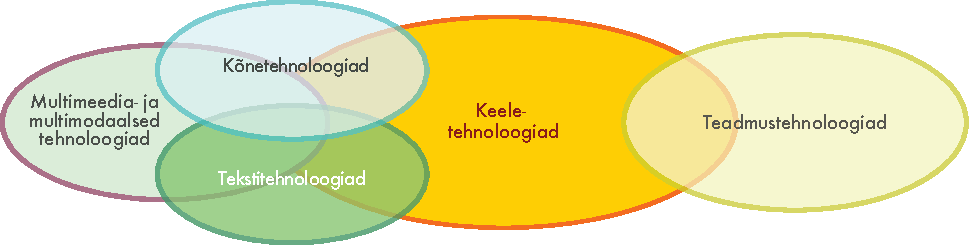
\includegraphics[width=\textwidth]{../_media/estonian/language_technologies}
  \caption{Keeletehnoloogia infotehnoloogia kontekstis}
  \label{fig:ltincontext_ee}
  \colorrule{grey3}{\textwidth}{1.5pt}
\end{figure*}

Järgnevalt vaatleme peamisi keeletehnoloogia rakenduste valdkondi: keeleline kontroll, veebiotsing, kõnetehnoloogia ja masintõlge. 
Nad hõlmavad rakendusi ja baastehnoloogiaid, nagu näiteks:

       \begin{itemize}
      \item õigekirjakontroll,
      \item kirjutaja abivahendid,
      \item arvutitoetatud keeleõpe,
      \item infootsing,
      \item info ekstraheerimine,
      \item automaatne sisukokkuvõtete tege\-mine,
      \item küsimustele vastamine,
      \item kõnetuvastus,
      \item kõnesüntees.
    \end{itemize}


Keeletehnoloogia on väljakujunenud uurimisala, millel on märkimisväärne hulk sissejuhatavat kirjandust. Huvitatud lugeja võib tutvuda järgmiste viidetega:  \cite{carstensen-etal1, jurafsky-martin01, manning-schuetze1, lt-world1, lt-survey1}.

Enne mainitud rakenduste tutvustamist kirjeldame tüüpilise keeletehnoloogilise süsteemi arhitektuuri. 


\subsection{Rakenduste arhitektuur}

Keeletöötlustarkvara komponendid vastavad keele erinevatele tahkudele. 
Joonis \ref{fig:textprocessingarch_ee} illustreerib tüüpilise tekstitöötlussüsteemi lihtsustatud arhitektuuri. 
Kolm esimest moodulit tegelevad tekstisisendi struktuuri ja tähendusega:

\begin{figure*}[htb]
  \colorrule{grey3}{\textwidth}{1.5pt}
  \center
  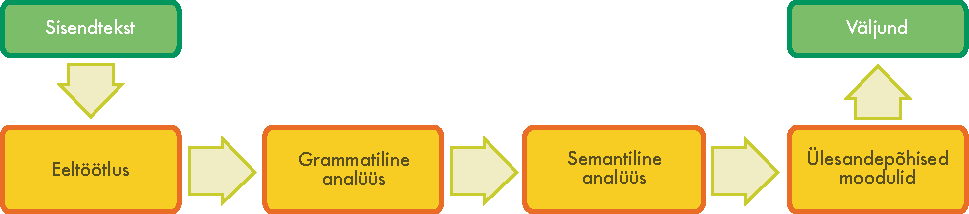
\includegraphics[width=\textwidth]{../_media/estonian/text_processing_app_architecture}
  \caption{Tüüpiline keeletöötluse arhitektuur}
  \label{fig:textprocessingarch_ee}
  \colorrule{grey3}{\textwidth}{1.5pt}
\end{figure*}

\begin{enumerate}
      \item Eeltöötlus puhastab andmed, ana\-lüüsib või eemaldab vorminduse, tuvastab sisendkeele  jne.
      \item Grammatiline analüüs leiab sõna\-liigid, öeldise, sihitise, laiendid, teised lauseliikmed ning tuvastab lause struktuuri.
      \item Semantilise analüüsi käigus toimub ühestamine (s.o sõnade konteksti sobivate tähenduste tuvastamine), anafooride lahendamine (nimisõnade vastavusse seadmine asesõnadega), väljendite asendamine ning lause tähenduse esitamine masinloetaval kujul.
\end{enumerate}

Tekstianalüüsi järel alustavad tööd ülesandespetsiifilised moodulid nagu automaatne sisukokkuvõtte tegija ja andmebaasiotsing. 
See lihtsustatud ja idealiseeritud kirjeldus näitlikustab keeletehnoloogiliste rakenduste arhitektuuri keerukust. 

Pärast kesksete keeletehnoloogiliste rakenduste tutvustamist anname ülevaate keeletehnoloogia-alasest uurimistööst ja haridusest ning olnud ja käimasolevatest uurimisprogrammidest. 
Anname ka eksperthinnangu kesksete rakenduste ja ressursside hetkeseisule erinevates kategooriates, näiteks kättesaadavus, küpsus ja kvaliteet. 
Tabelis võtame kokku eesti keele keeletehnoloogia üldise hetkeolukorra. 

\subsection{Kesksed rakendused} 

Selles peatükis keskendume kõige olulisemate keeletehnoloogiliste vahendite ja ressursside kirjeldamisele ja anname ülevaate keeletehnoloogia-alasest tegevusest Eestis. 
Tekstis rõhutatud vahendeid ja ressursse on kirjeldatud ka peatüki lõpus olevas tabelis.

\subsubsection{Keeleline kontroll}

Igaüks, kes on kasutanud tekstiredaktorit (nt Microsoft Word’i), teab, et sellel on olemas õigekirjakontrollija, mis joonib alla kirjavead ja annab soovitusi nende parandamiseks. 
Esimesed õigekirjakorrektorid (ehk spellerid) võrdlesid sisestatud sõnu leksikonis olevate korrektsete sõnadega. 
Tänapäevased spellerid on keerulisemad. 
Keelespetsiifilisi \textbf{grammatikaanalüüsi} algoritme kasutades leitakse morfoloogilised vead (nt mitmuse moodustamine), süntaksivead, näiteks lausest puuduv tegusõna või aluse ja öeldise ühildumise konflikt (nt \textit{nad kirjutas kirja}). 
Kuid enamik spellereid ei suuda leida vigu sellisest inglisekeelsest tekstist \cite{zar1} nagu: 
\begin{quote}
      I have a spelling checker,\\
      It came with my PC.\\
      It plane lee marks four my revue\\
      Miss steaks aye can knot sea 
\end{quote}

(Siin on tegemist sõnademänguga, sõnad on asendatud teiste samasuguse hääldusega sõnadega, nii et iga üksiku sõna kirjapilt on korrektne.)

Taoliste vigade tuvastamine vajab kontekstianalüüsi. 
Sageli juhtub, et hooletu näpulöök klaviatuuril jätab sõnast ära eesti keele mitmusetunnuse \textit{-d}: 

\begin{quote}
 \textit värvilise õied\\ 
 \textit värvilise\textbf{d} õied
\end{quote}

Sellist tüüpi vigade analüüs vajab kas ekspertide poolt käsitsi koostatud \textbf{grammatikat} ja seda kasutavat tarkvara või statistilisi keelemudeleid. 
Viimasel juhul arvutab mudel vastava sõna lauses paiknemise tõenäosuse (st sõna eelneva ja järgneva sõna vahel paiknemise tõenäosuse). 
Näiteks \textit{värvilise õie} on tunduvalt tõenäolisem sõnade järjend kui \textit{värvilise õied}. 
Samuti parandab speller otsinguteenuste päringuid, näiteks Google’i \textit{Kas mõtlesite …}-soovitused.

Automaatselt saab statistilist keelemudelit genereerida siis, kui on olemas suur (korrektsete) tekstide kogum (seda nimetatakse \textbf{tekstikorpuseks}). 
Kirjeldatud meetodeid on kasutatud inglise keele analüüsimiseks. 
Kahjuks ei ole nad otseselt eesti keelele ülekantavad, sest eesti keelel on vabam sõnajärg, peaaegu piiranguteta liitsõnade moodustamine ning suurem käände- ja pöördelõppude hulk. 

%!!!The use of language checking is not limited to word processors. It also applies to authoring support systems.

\boxtext{Keelelist kontrolli kasutatakse ka mujal kui tekstiredaktorites.}


\begin{figure*}[htb]
  \colorrule{grey3}{\textwidth}{1.5pt}
  \center
  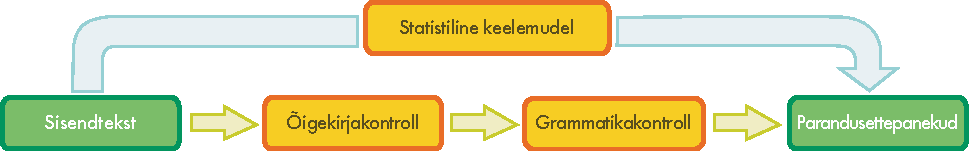
\includegraphics[width=\textwidth]{../_media/estonian/language_checking}
  \caption{Keeleline kontroll (üleval: statistiline; all: reeglipõhine)}
  \label{fig:langcheckingaarch_ee}
  \colorrule{grey3}{\textwidth}{1.5pt}
\end{figure*}

Eesti keele spelleri loomine algas 1991. aastal ning see on olnud tihedalt seotud eesti keele morfoloogiaanalüsaatori ESTMORF arenguga. 
Spelleri ja morfoloogiaanalüsaatori aluseks on 36000-sõnaline leksikon ja reeglid kõikide sõnavormide moodustamiseks. 
1994. aastal anti välja esimene versioon eesti keele spellerist. Hilisemates versioonides on leksikoni täiendatud nimede, lühendite ja neologismidega.

Speller on integreeritud kontoritarkvarapakettidesse MS Office, Open Office.org ja IBM Lotus Notes. 
Spellerit arendab era\-firma Filosoft OÜ \cite{Filosoft}.

Eesti keele jaoks on püütud luua ka teisi, vabavaralisi spellereid. 
Tuntuim neist on leksikon ispelli jaoks. 
Kahjuks ei suuda need spellerid piisavalt edukalt liitsõnu analüüsida.

Grammatikakontrollija kontrollib lause struktuuri ja punktuatsiooni. 
Eesti keele grammatikakontrollija arendustööga alustati Tartu Ülikoolis 2007. aastal.
Hetkel on olemas selle prototüüpversioon, mis suu\-dab tuvastada komavigu 95\% täpsusega.

Lisaks tekstiredaktorile kasutatakse keelelist kontrolli ka kirjutaja abivahendites. 
Need on tarkvarasüsteemid, millega koostatakse etteantud formaadis infotehnoloogia, meditsiini- ja tehnoloogiavaldkondade kasutajajuhendeid ning dokumentatsiooni. 
Ettevõtted on hakanud oluliselt suuremat tähelepanupöörama nii rahvusvahelise turu vajadustele tõlkimise ja lokaliseerimise vallas kui ka tehnilise dokumentatsiooni kvaliteedile. 
Kehvasti koostatud kasutusjuhendid põhjustavad toodete valesti kasutamist ning sellega kaasnevad klientide kahjunõuded. 
Keeletehnoloogia arengu käigus on loodud kirjutajaabivahendeid, mis aitavad tehnilise dokumentatsiooni koostajal kasutada piiratud sõnavara ja lausestruktuure, mis vastavad firma kehtestatud nõuetele ja (korporatiiv)terminoloogiale. 

Spellerite ja kirjutajaabivahendite kõrval vajab keelelist kontrolli ka arvutitoetatav keeleõpe. 

\subsubsection{Veebiotsing}

Keeletehnoloogia kõige laialtlevinum rakendus on otsing, nii veebis, sisevõrkudes kui ka digitaalsetes raamatukogudes. 
1998. aastast tegutsev Google’i otsingumootor teostab praegu umbes 80\% kõigist päringutest \cite{spi1}. 
2009. aastast alates on sõna guugeldama lisatud ka Eesti Õigekeelsussõnaraamatusse. 
Google’i otsinguliidese ja vastuse kuvamise lehekülje kujundus ei ole algusaegadega võrreldes oluliselt muutunud, kuid on toimunud sisulised muutused. 
Praegune versioon pakub valesti kirjutatud sõnadele õigekirjasoovitusi ning otsingu korrektsust parandab semantiline otsing, mis seisneb päringu konteksti sõnade tähenduste analüüsis \cite{pc1}. 
Google’i edulugu tõestab, et suure hulga andmete ja efektiivse indekseerimistehnikaga annab statistiline lähenemine häid tulemusi. 

\begin{figure*}[htb]
  \colorrule{grey3}{\textwidth}{1.5pt}
  \center
  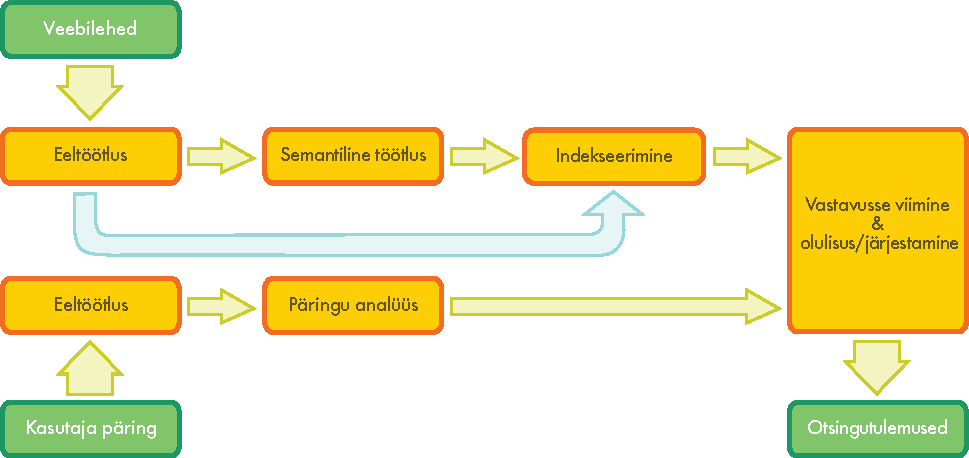
\includegraphics[width=\textwidth]{../_media/estonian/web_search_architecture}
  \caption{Veebiotsing}
  \label{fig:websearcharch_ee}
  \colorrule{grey3}{\textwidth}{1.5pt}
\end{figure*}

Keerulisema informatsioonivajaduse rahuldamiseks täiendatakse teksti tõlgendamise süsteeme sügavama lingvistilise teabega. 
Eksperimendid \textbf{leksikaalsete ressursside} (masinloetavad tesaurused või ontoloogilised keeleressursid, nt wordnet) kasutamiseks otsingutel on näidanud, et sobivate lehekülgede leidmine paraneb, sest leitakse ka sünonüüme ja nõrgemaid seosetüüpe sisaldavad lehed, näiteks on seotud \textit{aatomienergia} ja \textit{tuumaenergia}. 

Võtmesõnade nimekirja asemel küsimustena või muud tüüpi lausetena esitatud päringute töötlemiseks peaksid järgmise põlvkonna otsingumootorid sisaldama palju keerulisemat keeletehnoloogiat. 
Et vastata päringule ``Anna mulle nimekiri kõigist neist ettevõtetest, mille on teised ettevõtted viimase viie aasta jooksul üle võtnud'', peab KT süsteem tegema lauses nii süntaktilise kui ka \textbf{semantilise analüüsi} ning andma kiiresti vastavate dokumentide indeksi. 
Vastuse andmiseks tuleb kõigepealt analüüsida lause grammatilist struktuuri ja mõista, et kasutaja tahab just nimekirju ülevõetud ettevõtetest, mitte ettevõtete omandajatest. 
Rahuldamaks väljendit ``viimase viie aasta jooksul'', peab süsteem leidma sobiva aastate vahemiku. 
Seejärel tükk tüki haaval informatsiooni leidmiseks on vaja sobitada päring meeletu hulga struktureerimata andmetega. 
Kirjeldatud protsessi nimetatakse infootsinguks, see sisaldab nii otsimist kui ka leitud dokumentide järjestamist. 
Ettevõtete nimekirja genereerimiseks kasutatakse nimeüksuste tuvastamise protsessi, mille käigus tuvastab süsteem dokumentidest ettevõtte nimeks sobiva sõnajärjendi. 


\boxtext{Järgmise põlvkonna otsimootorid peavad kasutama palju keerulisemat keeletehnoloogiat.}

Tunduvalt keerulisem on leida päringule vastust teises keeles olevate dokumentide hulgast. 
Keeltevaheline infootsing eeldab päringu automaatset tõlkimist kõigisse võimalikesse lähtekeeltesse ja hiljem saadud tulemuste tõlkimist sihtkeelde. 

Tänapäeval suureneb pidevalt andmete hulk, mis esinevad mingil muul kujul kui kirjalik tekst ja on tekkinud vajadus multimeedia infootsingu teenuse järele, mis otsiks pilte, audiofaile ja videoandmeid. 
Audio-ja videofailidest otsimiseks teisendab kõnetuvastusmoodul kõne tekstiks või selle foneetiliseks esituseks, mida saab kasutaja päringuga sobitada. 

Keelest sõltumatud otsinguvahendid suudavad leida ainult sõnavorme, millel on päringusõnaga täpselt sama kuju või mis sisaldavad päringusõna alamsõnena. 
Kuna eesti keele morfoloogia on rikas ja lisaks lõppudele võib ka sõna tüvi muutuda, siis on edukaks otsinguks ja indekseerimiseks vaja keelespetsiifilisi vahendeid. 

Dokumente hoitakse arvutis kui suur tekstilist andmebaasi. 
Täistekstiotsing jagatakse kaheks alamülesandeks: indekseerimiseks ja otsimiseks. 
Indekseerimise protsessis analüüsitakse tekste sõna-sõnalt ja luuakse otsisõnade nimekiri ehk indeks. 
Otsimisfaasis kasutatakse konkreetse päringu töötlemiseks ainult indeksit, mitte kogu teksti. 
Indekseerija loob kirje iga dokumendist leitud sõna või termini jaoks, kirjesse salvestatakse ka dokumendi viide ja vahel ka selle sõna asukoht dokumendis.
Keelespetsiifilised indekseerijad leiavad enne sõnade indeksisse lisamist nende algvormid ehk lemmatiseerivad otsisõnad. 
Näiteks sõnavormid \textit{käsi}, \textit{käe}, \textit{kätt} esitatakse indeksis ainult tüvisõna ehk lemma \textit{käsi} kirjena. 
Mõnel juhul leiab lemmatiseerija ühele sõnavormile mitu algvormi, nt \textit{kuue} algvormideks on nii \textit{kuub} kui ka \textit{kuus}. 
Sellise mitmesuse lahendamiseks otsib süsteem sõnade konteksti põhjal õige algvormi (protsessi nimetatakse morfoloogiliseks ühestamiseks). 


Eesti Infosüsteemide Amet on avalikult soovitanud kasutada Eesti avaliku sektori infosüsteemide infootsingul ja indeksee\-rimisel lemmatiseerimismoodulit \cite{RIA}.

Esimene lemmatiseerijat kasutav otsingumootor oli kasutusel 1997--2001 aastal Riigi\-kantselei infosüsteemis.
Ka Google’i otsingu\-mootor kasutab eesti keele jaoks mõningast lemmatiseerimist, näiteks päringule \textit{majandusminister} antakse vastuses viiteid ka dokumentidele, milles esineb ainsuse omastavas käändes vorm \textit{majandus\-ministri}.

\subsubsection{Suuline suhtlus}

Suuline suhtlus on rakendusvaldkond, mis sõltub kõnetehnoloogiast ehk suulise keele töötlemise tehnoloogiast. 
Suulise suhtluse tehnoloogiat kasutatakse sellise kasutajaliidese loomiseks, kus traditsioonilise graafilise kujunduse, hiire ja klaviatuuri asemel suheldakse arvutiga suulist kõnet kasutades. 
Tänapäeval kasutatakse näiteks hääljuhitavaid kasutajaliideseid osaliselt või täielikult automatiseeritud telefoniteenustes. 
Hääljuhitavad kasutajaliidesed on kasutusel panganduses, tarneahelate juhtimises, ühistranspordis, telekommunikatsioonis ja teistes ärivaldkondades. 
Suulise suhtluse tehnoloogiat kasutatakse ka autode navigeerimissüsteemides ning nutitelefonides graafilise puutetundliku kasutajaliidese alternatiivina. 

%!!!Speech interaction is the basis for creating interfaces that allow a user to interact with spoken language instead of a graphical dis-play, keyboard and mouse.

\boxtext{Suulise suhtluse tehnoloogiat kasutatakse sellise kasutajaliidese loomiseks, kus traditsioonilise graafilise kujunduse, hiire ja klaviatuuri asemel suheldakse arvutiga suulist kõnet kasutades.}

\begin{figure*}[htb]
  \colorrule{grey3}{\textwidth}{1.5pt}
  \center 
  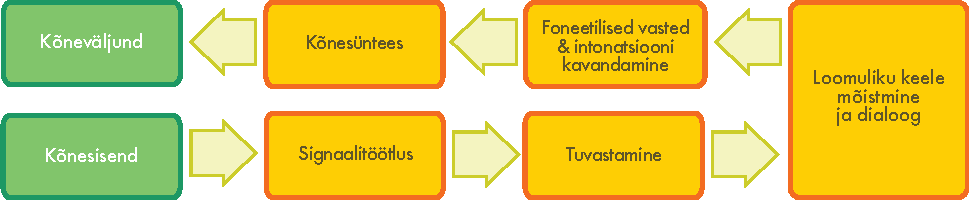
\includegraphics[width=\textwidth]{../_media/estonian/simple_speech-based_dialogue_architecture}
  \caption{Kõnepõhine dialoogsüsteem}
  \label{fig:dialoguearch_ee}
  \colorrule{grey3}{\textwidth}{1.5pt}
\end{figure*}


Suuline suhtlus hõlmab nelja tehnoloogiat:
   \begin{enumerate}
      \item Automaatne \textbf{kõnetuvastus} teeb kasutaja poolt kuuldavale toodud helijärjendi põhjal kindlaks tegelikult öeldud sõnad.
      \item Loomuliku keele mõistmise protsess ana\-lüüsib öeldu süntaktilist struk\-tuuri ja tõlgendab seda vastavalt süsteemi vajadustele.
      \item Dialoogi haldamise moodul määrab süsteemi funktsionaalsust arvestades selle, milline tegevus algatatakse vastuseks kasutaja sisendile. 
      \item \textbf{Kõnesüntees} teisendab süsteemi vastuse helideks.
    \end{enumerate}

Kõnetuvastussüsteemi suurimaks väljakutseks on kasutaja öeldud sõnade tuvastamine. 
Probleemi lahendamiseks piiratakse võimalike ütluste hulka konkreetsete võtmesõnadega või siis luuakse käsitsi rohkelt loomuliku keele ütlusi sisaldav keelemudel. 
Masinõppetehnoloogiaga on võimalik keelemudeleid ka automaatselt luua, selleks kasutatakse \textbf{kõnekorpust}, mis koosneb suurest hulgast kõnet sisaldavatest audiofailidest ja teksti transkriptsioonidest. 
Sõnavara piiramine sunnib inimesi kasutama väga jäika hääljuhitavat kasutajaliidest. 
Kasutajatele ei pruugi see küll meeldida, kuid samas rikkama sõnavaraga keelemudeli loomine, sobitamine ja ka haldamine on oluliselt kallim. 
Kasutajatele on vastuvõetavamad keelemudelil põhinevad kasutajaliidesed, mis lubavad neil oma soove võimalikult paindlikult väljendada, näiteks kasutajaliides alustab dialoogi lausega \textit{''Kuidas ma saan sind aidata?''}. 

Hääljuhitavate kasutajaliideste tootjad eelistavad väljundi genereerimisel kasutada eelsalvestatud professionaalsete diktorite ütlusi. 
Staatiliste ütluste korral, mil sõnastus ei sõltu kontekstist ega kasutaja andmetest, annab see parema tulemuse. 
Dünaamilise sisu korral on tulemus ebaloomuliku intonatsiooniga, sest audiofaili tükid liidetakse lihtsalt kokku. 
Tänapäeva kõnesünteesisüsteemides on loomulikult kõlavate dünaamiliste ütluste genereerimine muutunud üha paremaks, kuid arenguruumi veel on. 

Turul olevate kõnetehnoloogialiideste komponendid on viimase kümnendi jooksul standardiseerunud ning kõnetuvastuse ja kõnesünteesi turg on märkimisväärselt konsolideerunud. 
G20 riikide rahvuslikel turgudel domineerivad viis globaalset tegijat, Euroopas on neist tuntuimad Nuance (USA) ja Loquendo (Itaalia). 
2011. aastal teatas Nuance, et omandas Loquendo, see märgib konsolideerumise jätkumist.

Eesti keele automaatse kõnetuvastusega tegeleb peamiselt Tallinna Tehnikaülikooli Küberneetika Instituudi foneetika ja kõnetehnoloogia labor. 
2000. aastal valmis prototüüp isoleeritud sõnade tuvastamiseks (eestikeelsed numbrite ja tähtede nimetused), 2002--2004 valmis piiratud sõnavaraga peidetud Markovi mudelil (HMM) põhinev sidusa kõne tuvastussüsteem. 
Viimane kõnetuvastussüsteemi versioon (2010) võimaldab tuvastada piiramata sõnavara 63--85\% täpsusega. Tulemus sõltub kõne žanrist, sõnavarast ja signaali kvaliteedist (müra tasemest) \cite{Phon}.

On loodud kõnetuvastaja veebirakendus, mis võimaldab automaatselt transkribeeritud raadiovestlussaateid lehitseda, neid kuulata ja nendest otsida . 
Samuti on olemas veebiteenus, millega kasutaja saab saata süsteemile oma helifaile transkribeerimiseks. 
Arendamisjärgus on radioloogidele sobiva kõnetuvastussüsteemi loomine, millega on võimalik dikteerida ka spetsiifilisemat sõnavara. 
Esialgsed eksperimenditulemused on paljulubavad (10\% vigu reaalajalisel tuvastamisel). 

Aastatel 1997--2002 loodi kolme organisatsiooni (TTÜ Küberneetika Instituut, Eesti Keele Instituut ja OÜ Filosoft) poolt eesti keele tekst-kõnesüntesaator. 
See kõnesüntesaatori versioon kuulub n.ö süntesaatorite esimesse põlvkonda, kasutatakse difoone, iga kõneüksus vastab täpselt ühele andmebaasis olevale difoonile (helilt helile üleminekule). 
Süntesaatori väljund on arusaadav, kuid on monotoonne, veidi hakitud ja pisut ebaloomuliku kõlaga. 
Süntesaator on kohandatud  kasutamiseks pimedatele. 
Süntesaator on avatud lähtekoodiga, seda võib kasutada mitteärilistel ja mittesõjalistel eesmärkidel \cite{IEL}. 

Eesti Keele Instituut arendab hetkel ka korpusepõhise kõnesüntesaatori versiooni, milles lisaks difoonidele kasutatakse ka pikemaid kõneüksusi (sõnu ja fraase). 

Haridus- ja teadusministeeriumi parima keeleteo auhinna võitsid 2010. aastal MTÜ Jumalalaegas ja Eesti Hoiuraamatukogu töörühm, kes lõid eestikeelse hääljuhendamise pimedate tehnilistele abivahenditele. 
Nende rakendused kasutavad soome kõnesüntesaatorit. 

Tulevikus on oodata märkimisväärseid muutusi kõnetehnoloogia arengus. 
Kõnetehnoloogia kasutamist mõjutab ka laialt levima hakanud nutitelefon, mis on tavalise telefoniside, interneti ja e-maili kõrval uus sobiv platvorm kliendisuhete halduseks. 
Ilmselt on tulevikutelefonis vähem hääljuhitavaid kasutajaliideseid ning suuline kõne hakkab mängima nutitelefonides suuremat rolli kasutajasõbraliku sisendina. 
Arengu protsess sõltub kõnelejast sõltumatute kõnetuvastussüsteemide korrektsuse paranemisest. 
Juba praegu pakutakse nutitelefonide kasutajatele tsentraliseeritud teenustena kõne dikteerimist.
Sarnased Tanel Alumäe ja Kaarel Kaljuranna TTÜ Küberneetika Instituudis välja töötatud eestikeelsed kõnetuvastusrakendused nutitelefonidele võitsid 2011. aasta parima keeleteo auhinna.


\subsubsection{Masintõlge}

Mõte kasutada arvuteid loomuliku keele tõlkimiseks tekkis juba 1946. aastal. 
Olulisel määral rahastati seda uurimissuunda viiekümnendatel ja kaheksakümnendatel aastatel, kuid vaatamata pikale ajaloole ei täida isegi tänapäevane \textbf{masintõlge} algselt talle seatud eesmärki, milleks oli automaatne piirideta tõlge. 

%!!!At its basic level, Machine Translation simply substitutes words in one natural language with words in another language.



Kõige sirgjoonelisem masintõlke viis seisneb ühe keele sõnade asendamises teise keele sõnadega. 
Selline lähenemine sobib piiratud sõnavaraga valdkondade tekstide (nt ilmateadete) tõlkimiseks. 
Vähem standardiseeritud teksti kvaliteetseks tõlkeks on vajalik suuremale tekstiüksusele (fraasile, lausele või tervele lõigule) sobiva sihtkeelse vaste leidmine. 

\boxtext{Kõige sirgjoonelisem masintõlke viis seisneb ühe keele sõnade asendamises teise keele sõnadega.}

Peamiseks takistuseks on inimkeele mitmesus, mis esitab väljakutse erinevatel analüüsitasanditel, näiteks sõnatähenduse mitmesus leksikaalsel tasandil (\textit{hiir} võib olla nii loom kui arvuti osa) või lause struktuuri mitmesus süntaktilisel tasandil, vt alljärgnevaid tõlkeid inglise keelest: 

\begin{quote}
\textit{The woman saw the car and her husband, too.\\
{[}Naine nägi autot ja tema abikaasa samuti.{]}\\
{[}Naine nägi autot ja samuti oma abikaasat.{]}}
\end{quote}

Masintõlkesüsteem võib põhineda ka lingvistilistel reeglitel. 
Lähedalt seotud keelte tõlkimisel saab kasutada otsest asendamist. 
Reeglipõhised (või lingvistiliste teadmiste põhised) masintõlkesüsteemid analüüsivad lähtekeelset teksti ning loovad selle põhjal vahepealse sümbolilise esituse hilisemaks sihtkeelsesse teksti genereerimiseks. 
Taolised süsteemid vajavad heaks tõlkeks nii põhjalikke leksikone, milles on esitatud morfoloogiline, süntaktiline ja semantiline informatsioon kui ka mahukaid käsitsi koostatud grammatikaid. 
Vajalike vahendite loomise protsess on pikk ja seetõttu ka kallis. 

\begin{figure*}[htb]
  \colorrule{grey3}{\textwidth}{1.5pt}
  \center
  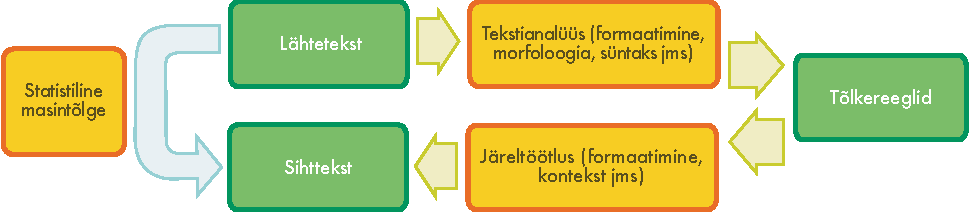
\includegraphics[width=\textwidth]{../_media/estonian/machine_translation}
  \caption{Masintõlge (vasakul: statistiline; paremal: reeglipõhine)}
  \label{fig:mtarch_ee}
  \colorrule{grey3}{\textwidth}{1.5pt}
\end{figure*}

Hilistel kaheksakümnendatel, kui arvutusvõimsus suurenes ja ühtlasi ka odavnes, tekkis huvi statistiliste masintõlkemudelite loomise vastu. 
Statistilised mudelid saadakse kakskeelsete tekstikorpuste analüüsil. 
Näiteks Europarli \textbf{paralleelkorpus} sisaldab Euroopa Parlamendi väljaandeid 11 Euroopa keeles. 
Piisava andmehulga korral leiab masintõlkesüsteem võõrkeelsele tekstile sellise tõlke, mis annab edasi teksti ligikaudse tähenduse. 
Erinevalt reeglipõhistest süsteemidest genereerib statistiline masintõlkesüsteem sageli grammatiliselt mittekorrektse väljundi. 
Samas statistilise süsteemi loomiseks on vaja vähem inimtööjõudu ning see katab ka teatud keele eripärasid (nt idiomaatilised väljendid), mida teadmistepõhised süsteemid ignoreerivad. 

\boxtext{Eesti keele masintõlge on tõsine väljakutse.} 

Statistiliste ja reeglipõhiste masintõlkesüsteemide tugevad ja nõrgad küljed kompenseerivad üksteist, seetõttu pööratakse hetkel suurt tähelepanu mõlemat lähenemist kombineerivale hübriidsele meetodile. 
Üheks selle rakendamise võimaluseks on tõlkida paralleelselt lingvistilist ja statistilist tõlget kasutades ja hiljem valikumoodulis otsustada, kumb tõlge on parem. 
Pikemate lausete (üle 12 sõna) korral on tulemused perfektsusest kaugel. 
Kvaliteetsema tulemuse saaks kombineerides kummagi tõlke parimaid osi, samas on see küllaltki keeruline ning alati ei ilmne omavahel täpses vastavuses olevad osad. 



Eesti keele masintõlge on tõsine väljakutse. 
Sõnastikupõhise analüüsi muudab keeruliseks vaba liitsõnamoodustus, uusi sõnu saab liitmise teel alati juurde tekitada. 
Analüüsiprobleeme põhjustavad ka vaba sõnajärg ja mitmeosalised tegusõnad (ühend- ning väljendverbid). 
Lisaks kõigele muule on piiratud ka paralleelsete tekstide hulk. 
Vaatamata sellele kuulub Eesti keel nende ligi 50 maailma keele hulka, mida saab arvuti abil tõlkida \cite{Koit}.

Eesti keele masintõlke ajalugu ulatub tagasi 50ndatesse, kui Tartu Ülikooli matemaatikud katsetasid matemaatiliste tekstide tõlkimist vene keelest eesti keelde. 
Tolleaegne riistvara (arvuti Ural) töötas kiirusega 100 operatsiooni sekundis. Nõrk arvutusvõimsus oligi üks katsete katkestamise põhjustest. 

Praegu on eesti keele jaoks olemas kaks masintõlkesüsteemi. 
Tuntuim neist on Google’i tõlketeenus. 
Selle kvaliteet ei ole küll alati küllaldane, kuid võimaldab \mbox{siiski} aru saada teksti üldisest teemast ja põhifaktidest.

Teist masintõlkesüsteemi arendab Tartu Ülikooli uurimisgrupp. 
Nende uurimistöö keskendub hetkel eesti-inglise masintõlkesuunale. 
Süsteem (masintolge.ut.ee) tõlgib piiratud pikkusega lauseid eesti keelest inglise keelde. 
Masintõlkesüsteem kasutab avatud lähtekoodiga Mosese dekodeerimismooduleid ja seda treenitakse erinevatel eesti-inglise paralleelkorpustel, kaasa arvatud JRC-Acquis ning OPUS. 

Masintõlkesüsteem suurendab oluliselt töö produktiivsust, eriti siis, kui süsteem on integreeritud töövoogu ning kohandatud kasutajaspetsiifilise terminoloogiaga. 
Näiteks Siemens kasutab interaktiivset tõlget toetavaid süsteeme ja Volkswagen kasutab keeleportaali, mis tagab ligipääsu sõnaraamatutele, ettevõttespetsiifilisele terminoloogiale, tõlkemälule ja masintõlketoele. 

Masintõlkesüsteemide kvaliteedi parandamisel on veel palju arenguruumi. 
Väljakutseks on keeleressursside kohandamine konkreetse sektori vajadustega ning tehnoloogia integreerimine töövoo protsessidesse, mis juba kasutavad terminoloogiabaasi ja tõlkemälu. 

Hindamiskampaaniad võrdlevad masintõlkesüsteemide kvaliteeti, erinevaid lähenemisi ja süsteemide eri keelepaaride olukorda. 
Euromatrix+ projekti käigus loodud tabelis (vt joonis~\ref{fig:euromatrix_de}) on koondatud keelepaariti (iiri keelt ei võrreldud) 22 ELi ametliku keele tulemused. 
Tulemusi on hinnatud BLEU-punktidega, milles parema tõlke skoor on alati kõrgem \cite{bleu1}. 
Inimtõlkija koguks ülesandest keskmiselt 80 punkti. 
Parimad punktisummad (tabelis rohelise ja sinise värviga tähistatud) said keeled, millesse on koostööprojektides palju panustatud ning mille jaoks leidub rohkelt paralleeltekste (nt inglise, prantsuse, hollandi, hispaania ja saksa keel). 
Tabelis on punasega märgitud halvimad tulemused. 
Nendele keeltele kas ei ole piisavalt tähelepanu pööratud või need keeled erinevad struktuurilt oluliselt teistest keeltest (näiteks ungari, malta, soome keel ja eesti keel). 

\begin{figure*}[htbp]
  \centering
  \setlength{\tabcolsep}{0.17em}
  \small
  \begin{tabular}{>{\columncolor{corange1}}cccccccccccccccccccccccc}
    & \multicolumn{22}{>{\columncolor{corange1}}c}{Sihtkeeled -- \textcolor{grey1}{Target language}}\\\addlinespace[{-.009cm}]
    \rowcolor{corange1}  & EN & BG & DE & CS & DA & EL & ES & ET & FI & FR & HU & IT & LT & LV & MT & NL & PL & PT & RO & SK & SL & SV\\
    EN & -- & \textcolor{blue}{40.5} & \textcolor{blue}{46.8} & \textcolor{green2}{52.6} & \textcolor{green2}{50.0} & \textcolor{blue}{41.0} & \textcolor{green2}{55.2} & \textcolor{purple}{34.8} & \textcolor{purple}{38.6} & \textcolor{green2}{50.1} & \textcolor{purple}{37.2} & \textcolor{green2}{50.4} & \textcolor{purple}{39.6} & \textcolor{blue}{43.4} & \textcolor{purple}{39.8} & \textcolor{green2}{52.3} & \textcolor{blue}{49.2} & \textcolor{green2}{55.0} & \textcolor{blue}{49.0} & \textcolor{blue}{44.7} & \textcolor{green2}{50.7} & \textcolor{green2}{52.0}\\
    BG & \textcolor{green}{61.3} & -- & \textcolor{purple}{38.7} & \textcolor{purple}{39.4} & \textcolor{purple}{39.6} & \textcolor{purple}{34.5} & \textcolor{blue}{46.9} & \textcolor{red3}{25.5} & \textcolor{red3}{26.7} & \textcolor{blue}{42.4} & \textcolor{red3}{22.0} & \textcolor{blue}{43.5} & \textcolor{red3}{29.3} & \textcolor{red3}{29.1} & \textcolor{red3}{25.9} & \textcolor{blue}{44.9} & \textcolor{purple}{35.1} & \textcolor{blue}{45.9} & \textcolor{purple}{36.8} & \textcolor{purple}{34.1} & \textcolor{purple}{34.1} & \textcolor{purple}{39.9}\\
    DE & \textcolor{green2}{53.6} & \textcolor{red3}{26.3} & -- & \textcolor{purple}{35.4} & \textcolor{blue}{43.1} & \textcolor{purple}{32.8} & \textcolor{blue}{47.1} & \textcolor{red3}{26.7} & \textcolor{red3}{29.5} & \textcolor{purple}{39.4} & \textcolor{red3}{27.6} & \textcolor{blue}{42.7} & \textcolor{red3}{27.6} & \textcolor{purple}{30.3} & \textcolor{red2}{19.8} & \textcolor{green2}{50.2} & \textcolor{purple}{30.2} & \textcolor{blue}{44.1} & \textcolor{purple}{30.7} & \textcolor{red3}{29.4} & \textcolor{purple}{31.4} & \textcolor{blue}{41.2}\\
    CS & \textcolor{green2}{58.4} & \textcolor{purple}{32.0} & \textcolor{blue}{42.6} & -- & \textcolor{blue}{43.6} & \textcolor{purple}{34.6} & \textcolor{blue}{48.9} & \textcolor{purple}{30.7} & \textcolor{purple}{30.5} & \textcolor{blue}{41.6} & \textcolor{red3}{27.4} & \textcolor{blue}{44.3} & \textcolor{purple}{34.5} & \textcolor{purple}{35.8} & \textcolor{red3}{26.3} & \textcolor{blue}{46.5} & \textcolor{purple}{39.2} & \textcolor{blue}{45.7} & \textcolor{purple}{36.5} & \textcolor{blue}{43.6} & \textcolor{blue}{41.3} & \textcolor{blue}{42.9}\\
    DA & \textcolor{green2}{57.6} & \textcolor{red3}{28.7} & \textcolor{blue}{44.1} & \textcolor{purple}{35.7} & -- & \textcolor{purple}{34.3} & \textcolor{blue}{47.5} & \textcolor{red3}{27.8} & \textcolor{purple}{31.6} & \textcolor{blue}{41.3} & \textcolor{red3}{24.2} & \textcolor{blue}{43.8} & \textcolor{red3}{29.7} & \textcolor{purple}{32.9} & \textcolor{red3}{21.1} & \textcolor{blue}{48.5} & \textcolor{purple}{34.3} & \textcolor{blue}{45.4} & \textcolor{purple}{33.9} & \textcolor{purple}{33.0} & \textcolor{purple}{36.2} & \textcolor{blue}{47.2}\\
    EL & \textcolor{green2}{59.5} & \textcolor{purple}{32.4} & \textcolor{blue}{43.1} & \textcolor{purple}{37.7} & \textcolor{blue}{44.5} & -- & \textcolor{green2}{54.0} & \textcolor{red3}{26.5} & \textcolor{red3}{29.0} & \textcolor{blue}{48.3} & \textcolor{red3}{23.7} & \textcolor{blue}{49.6} & \textcolor{red3}{29.0} & \textcolor{purple}{32.6} & \textcolor{red3}{23.8} & \textcolor{blue}{48.9} & \textcolor{purple}{34.2} & \textcolor{green2}{52.5} & \textcolor{purple}{37.2} & \textcolor{purple}{33.1} & \textcolor{purple}{36.3} & \textcolor{blue}{43.3}\\
    ES & \textcolor{green}{60.0} & \textcolor{purple}{31.1} & \textcolor{blue}{42.7} & \textcolor{purple}{37.5} & \textcolor{blue}{44.4} & \textcolor{purple}{39.4} & -- & \textcolor{red3}{25.4} & \textcolor{red3}{28.5} & \textcolor{green2}{51.3} & \textcolor{red3}{24.0} & \textcolor{green2}{51.7} & \textcolor{red3}{26.8} & \textcolor{purple}{30.5} & \textcolor{red3}{24.6} & \textcolor{blue}{48.8} & \textcolor{purple}{33.9} & \textcolor{green2}{57.3} & \textcolor{purple}{38.1} & \textcolor{purple}{31.7} & \textcolor{purple}{33.9} & \textcolor{blue}{43.7}\\
    ET & \textcolor{green2}{52.0} & \textcolor{red3}{24.6} & \textcolor{purple}{37.3} & \textcolor{purple}{35.2} & \textcolor{purple}{37.8} & \textcolor{red3}{28.2} & \textcolor{blue}{40.4} & -- & \textcolor{purple}{37.7} & \textcolor{purple}{33.4} & \textcolor{purple}{30.9} & \textcolor{purple}{37.0} & \textcolor{purple}{35.0} & \textcolor{purple}{36.9} & \textcolor{red3}{20.5} & \textcolor{blue}{41.3} & \textcolor{purple}{32.0} & \textcolor{purple}{37.8} & \textcolor{red3}{28.0} & \textcolor{purple}{30.6} & \textcolor{purple}{32.9} & \textcolor{purple}{37.3}\\
    FI & \textcolor{blue}{49.3} & \textcolor{red3}{23.2} & \textcolor{purple}{36.0} & \textcolor{purple}{32.0} & \textcolor{purple}{37.9} & \textcolor{red3}{27.2} & \textcolor{purple}{39.7} & \textcolor{purple}{34.9} & -- & \textcolor{red3}{29.5} & \textcolor{red3}{27.2} & \textcolor{purple}{36.6} & \textcolor{purple}{30.5} & \textcolor{purple}{32.5} & \textcolor{red2}{19.4} & \textcolor{blue}{40.6} & \textcolor{red3}{28.8} & \textcolor{purple}{37.5} & \textcolor{red3}{26.5} & \textcolor{red3}{27.3} & \textcolor{red3}{28.2} & \textcolor{purple}{37.6}\\
    FR & \textcolor{green}{64.0} & \textcolor{purple}{34.5} & \textcolor{blue}{45.1} & \textcolor{purple}{39.5} & \textcolor{blue}{47.4} & \textcolor{blue}{42.8} & \textcolor{green}{60.9} & \textcolor{red3}{26.7} & \textcolor{purple}{30.0} & -- & \textcolor{red3}{25.5} & \textcolor{green2}{56.1} & \textcolor{red3}{28.3} & \textcolor{purple}{31.9} & \textcolor{red3}{25.3} & \textcolor{green2}{51.6} & \textcolor{purple}{35.7} & \textcolor{green}{61.0} & \textcolor{blue}{43.8} & \textcolor{purple}{33.1} & \textcolor{purple}{35.6} & \textcolor{blue}{45.8}\\
    HU & \textcolor{blue}{48.0} & \textcolor{red3}{24.7} & \textcolor{purple}{34.3} & \textcolor{purple}{30.0} & \textcolor{purple}{33.0} & \textcolor{red3}{25.5} & \textcolor{purple}{34.1} & \textcolor{red3}{29.6} & \textcolor{red3}{29.4} & \textcolor{purple}{30.7} & -- & \textcolor{purple}{33.5} & \textcolor{red3}{29.6} & \textcolor{purple}{31.9} & \textcolor{red2}{18.1} & \textcolor{purple}{36.1} & \textcolor{red3}{29.8} & \textcolor{purple}{34.2} & \textcolor{red3}{25.7} & \textcolor{red3}{25.6} & \textcolor{red3}{28.2} & \textcolor{purple}{30.5}\\
    IT & \textcolor{green}{61.0} & \textcolor{purple}{32.1} & \textcolor{blue}{44.3} & \textcolor{purple}{38.9} & \textcolor{blue}{45.8} & \textcolor{blue}{40.6} & \textcolor{red3}{26.9} & \textcolor{red3}{25.0} & \textcolor{red3}{29.7} & \textcolor{green2}{52.7} & \textcolor{red3}{24.2} & -- & \textcolor{red3}{29.4} & \textcolor{purple}{32.6} & \textcolor{red3}{24.6} & \textcolor{green2}{50.5} & \textcolor{purple}{35.2} & \textcolor{green2}{56.5} & \textcolor{purple}{39.3} & \textcolor{purple}{32.5} & \textcolor{purple}{34.7} & \textcolor{blue}{44.3}\\
    LT & \textcolor{green2}{51.8} & \textcolor{red3}{27.6} & \textcolor{purple}{33.9} & \textcolor{purple}{37.0} & \textcolor{purple}{36.8} & \textcolor{red3}{26.5} & \textcolor{red3}{21.1} & \textcolor{purple}{34.2} & \textcolor{purple}{32.0} & \textcolor{purple}{34.4} & \textcolor{red3}{28.5} & \textcolor{purple}{36.8} & -- & \textcolor{blue}{40.1} & \textcolor{red3}{22.2} & \textcolor{purple}{38.1} & \textcolor{purple}{31.6} & \textcolor{purple}{31.6} & \textcolor{red3}{29.3} & \textcolor{purple}{31.8} & \textcolor{purple}{35.3} & \textcolor{purple}{35.3}\\
    LV & \textcolor{green2}{54.0} & \textcolor{red3}{29.1} & \textcolor{purple}{35.0} & \textcolor{purple}{37.8} & \textcolor{purple}{38.5} & \textcolor{red3}{29.7} & \textcolor{red2}{8.0} & \textcolor{purple}{34.2} & \textcolor{purple}{32.4} & \textcolor{purple}{35.6} & \textcolor{red3}{29.3} & \textcolor{purple}{38.9} & \textcolor{purple}{38.4} & -- & \textcolor{red3}{23.3} & \textcolor{blue}{41.5} & \textcolor{purple}{34.4} & \textcolor{purple}{39.6} & \textcolor{purple}{31.0} & \textcolor{purple}{33.3} & \textcolor{purple}{37.1} & \textcolor{purple}{38.0}\\
    MT & \textcolor{green}{72.1} & \textcolor{purple}{32.2} & \textcolor{purple}{37.2} & \textcolor{purple}{37.9} & \textcolor{purple}{38.9} & \textcolor{purple}{33.7} & \textcolor{blue}{48.7} & \textcolor{red3}{26.9} & \textcolor{red3}{25.8} & \textcolor{blue}{42.4} & \textcolor{red3}{22.4} & \textcolor{blue}{43.7} & \textcolor{purple}{30.2} & \textcolor{purple}{33.2} & -- & \textcolor{blue}{44.0} & \textcolor{purple}{37.1} & \textcolor{blue}{45.9} & \textcolor{purple}{38.9} & \textcolor{purple}{35.8} & \textcolor{blue}{40.0} & \textcolor{blue}{41.6}\\
    NL & \textcolor{green2}{56.9} & \textcolor{red3}{29.3} & \textcolor{blue}{46.9} & \textcolor{purple}{37.0} & \textcolor{blue}{45.4} & \textcolor{purple}{35.3} & \textcolor{blue}{49.7} & \textcolor{red3}{27.5} & \textcolor{red3}{29.8} & \textcolor{blue}{43.4} & \textcolor{red3}{25.3} & \textcolor{blue}{44.5} & \textcolor{red3}{28.6} & \textcolor{purple}{31.7} & \textcolor{red3}{22.0} & -- & \textcolor{purple}{32.0} & \textcolor{blue}{47.7} & \textcolor{purple}{33.0} & \textcolor{purple}{30.1} & \textcolor{purple}{34.6} & \textcolor{blue}{43.6}\\
    PL & \textcolor{green}{60.8} & \textcolor{purple}{31.5} & \textcolor{blue}{40.2} & \textcolor{blue}{44.2} & \textcolor{blue}{42.1} & \textcolor{purple}{34.2} & \textcolor{blue}{46.2} & \textcolor{red3}{29.2} & \textcolor{red3}{29.0} & \textcolor{blue}{40.0} & \textcolor{red3}{24.5} & \textcolor{blue}{43.2} & \textcolor{purple}{33.2} & \textcolor{purple}{35.6} & \textcolor{red3}{27.9} & \textcolor{blue}{44.8} & -- & \textcolor{blue}{44.1} & \textcolor{purple}{38.2} & \textcolor{purple}{38.2} & \textcolor{purple}{39.8} & \textcolor{blue}{42.1}\\
    PT & \textcolor{green}{60.7} & \textcolor{purple}{31.4} & \textcolor{blue}{42.9} & \textcolor{purple}{38.4} & \textcolor{blue}{42.8} & \textcolor{blue}{40.2} & \textcolor{green}{60.7} & \textcolor{red3}{26.4} & \textcolor{red3}{29.2} & \textcolor{green2}{53.2} & \textcolor{red3}{23.8} & \textcolor{green2}{52.8} & \textcolor{red3}{28.0} & \textcolor{purple}{31.5} & \textcolor{red3}{24.8} & \textcolor{blue}{49.3} & \textcolor{purple}{34.5} & -- & \textcolor{purple}{39.4} & \textcolor{purple}{32.1} & \textcolor{purple}{34.4} & \textcolor{blue}{43.9}\\
    RO & \textcolor{green}{60.8} & \textcolor{purple}{33.1} & \textcolor{purple}{38.5} & \textcolor{purple}{37.8} & \textcolor{blue}{40.3} & \textcolor{purple}{35.6} & \textcolor{green2}{50.4} & \textcolor{red3}{24.6} & \textcolor{red3}{26.2} & \textcolor{blue}{46.5} & \textcolor{red3}{25.0} & \textcolor{blue}{44.8} & \textcolor{red3}{28.4} & \textcolor{red3}{29.9} & \textcolor{red3}{28.7} & \textcolor{blue}{43.0} & \textcolor{purple}{35.8} & \textcolor{blue}{48.5} & -- & \textcolor{purple}{31.5} & \textcolor{purple}{35.1} & \textcolor{purple}{39.4}\\
    SK & \textcolor{green}{60.8} & \textcolor{purple}{32.6} & \textcolor{purple}{39.4} & \textcolor{blue}{48.1} & \textcolor{blue}{41.0} & \textcolor{purple}{33.3} & \textcolor{blue}{46.2} & \textcolor{red3}{29.8} & \textcolor{red3}{28.4} & \textcolor{purple}{39.4} & \textcolor{red3}{27.4} & \textcolor{blue}{41.8} & \textcolor{purple}{33.8} & \textcolor{purple}{36.7} & \textcolor{red3}{28.5} & \textcolor{blue}{44.4} & \textcolor{purple}{39.0} & \textcolor{blue}{43.3} & \textcolor{purple}{35.3} & -- & \textcolor{blue}{42.6} & \textcolor{blue}{41.8}\\
    SL & \textcolor{green}{61.0} & \textcolor{purple}{33.1} & \textcolor{purple}{37.9} & \textcolor{blue}{43.5} & \textcolor{blue}{42.6} & \textcolor{purple}{34.0} & \textcolor{blue}{47.0} & \textcolor{purple}{31.1} & \textcolor{red3}{28.8} & \textcolor{purple}{38.2} & \textcolor{red3}{25.7} & \textcolor{blue}{42.3} & \textcolor{purple}{34.6} & \textcolor{purple}{37.3} & \textcolor{purple}{30.0} & \textcolor{blue}{45.9} & \textcolor{purple}{38.2} & \textcolor{blue}{44.1} & \textcolor{purple}{35.8} & \textcolor{purple}{38.9} & -- & \textcolor{blue}{42.7}\\
    SV & \textcolor{green2}{58.5} & \textcolor{red3}{26.9} & \textcolor{blue}{41.0} & \textcolor{purple}{35.6} & \textcolor{blue}{46.6} & \textcolor{purple}{33.3} & \textcolor{blue}{46.6} & \textcolor{red3}{27.4} & \textcolor{purple}{30.9} & \textcolor{purple}{38.9} & \textcolor{red3}{22.7} & \textcolor{blue}{42.0} & \textcolor{red3}{28.2} & \textcolor{purple}{31.0} & \textcolor{red3}{23.7} & \textcolor{blue}{45.6} & \textcolor{purple}{32.2} & \textcolor{blue}{44.2} & \textcolor{purple}{32.7} & \textcolor{purple}{31.3} & \textcolor{purple}{33.5} & --\\
    \end{tabular}
  \caption{Masintõlge 22 Euroopa Liidu keele vahel -- \textcolor{grey1}{Machine translation between 22 EU-languages \cite{euro1}}}
  \label{fig:euromatrix_de}
\end{figure*}

\subsection{Muud rakendusalad}

Keeletehnoloogiliste rakenduste loomisel tuleb lahendada suur hulk süsteemis paiknevaid alamülesandeid, mida vahel ei ole kasutajaga suhtlemisel isegi näha. 
Need moodulid on vastavuses arvutilingvistika erinevate alamteemade uurimisobjektidega. 


%!!!Language technology applications often provide significant service functionalities ”behind the scenes” of larger software systems.

\boxtext{Keeletehnoloogilised rakendused on sageli suuremate tarkvarasüsteemide osad, tõstes nende funktsionaalsust kulisside tagant.}

Näiteks on aktiivne uurimisteema küsimustele vastamine, selle jaoks luuakse eraldi märgendatud korpusi ning korraldatakse teaduslikke võistlusi. 
Küsimustele vastamise kontseptsioon arenes välja võtmesõnadepõhisest otsingust, mille korral väljastab otsingumootor vastuseks sobivad dokumendid. 
Idee kohaselt esitab kasutaja konkreetse küsimuse, millele süsteem annab ühe vastuse.

\begin{quote}
Näiteks:
\textit{Küsimus: Kui vana oli Neil Armstrong sel ajal, kui ta astus Kuu pinnale?\\
Vastus: 38.}\\
\end{quote}

Kuigi ilmselgelt kuulub küsimustele vastamine veebiotsingu valdkonda, on see praegu katusterminiks sellistele uurimisteemadele nagu küsimuste erinevad liigid, nende käsitlemine ja oletatavat vastet sisaldavate dokumentide analüüsimine ja võrdlemine (kas nad annavad vastandlikke vastuseid?) ning konteksti ignoreerimata spetsiifilise informatsiooni (vastuse) tekstist välja filtreerimine. 

Eelnev on omakorda seotud informatsiooni ekstraheerimise (IE, kasutatakse ka mõistet info kurnamine) valdkonnaga, mis oli väga populaarne ja oluline 90ndate alguses, mil arvutilingvistikas hakati eelistama statistilisi meetodeid. 
IE eesmärgiks on dokumentidest väikeste spetsiifiliste infokildude tuvastamine, näiteks tuvastada uudisartiklitest firmade ülevõtmise põhitegijad. 
Teine tuntud ülesanne seisneb terroriaktide identifitseerimises. 
Tekstis leiduv info esitatakse tabelina, milles on näidatud akti sooritaja, sihtmärk, aeg, koht ja intsidendi tulemus. 
IE keskseks teemaks on valdkonnaspetsiifilise vormi täitmine andmetega. 
IE on üks näide tagaplaanil töötavast tehnoloogiast, mida saab praktikas erinevatesse rakenduskeskkondadesse lõimida. 

Automaatne sisukokkuvõtete tegemine ja teksti genereerimine on kaks sellist piiripealset ala, mille rakendused toimivad nii iseseisvate programmidena kui ka toetavas rollis n.ö kulisside taga. 
Automaatse sisukokkuvõtete tegemise käigus leitakse pikast tekstist oluline informatsioon ja esitatakse see lühema tekstina. 
Seda võimalust pakub ka näiteks tekstiredaktor Microsoft Word. 
Statistilisi meetodeid kasutatakse teksti oluliste sõnade (sõnad, mis esinevad tekstis väga sageli, kuid ei ole nii sagedased tavalises keelekasutuses) kindlaks tegemiseks ja enim neid olulisi sõnu sisaldavate lausete leidmiseks. 
Teksti sisukokkuvõttena esitataksegi just need laused. 
Kuna sisukokkuvõtte tekst koosneb muutmata kujul algse teksti lausetest, siis on kirjeldatud stsenaariumi järgivad programmid pigem tekstist lausete ekstraheerijad, väljavõtete tegijad.
Teiseks võimaluseks on genereerida täiesti uusi lauseid, mida lähtetekstis ei leidu. 
See lähenemine nõuab aga teksti sügavamat mõistmist ning seetõttu ei ole ta ei piisavalt robustne ega veakindel. 

Teksti genereerimise programmid on harva iseseisvad rakendused. Enamasti on nad integreeritud suurematesse tarkvarasüsteemidesse, näiteks haiglate info- süsteemi, mis kogub, salvestab ja töötleb patsientide andmeid. 
Andmete põhjal aruannete koostamine on üks paljudest sisukokkuvõtte tegemise rakendustest. 

Eesti keele jaoks leidub sisukokkuvõtete tegemiseks ainult prototüüpvahend. 
Eesti keele automaatne sisukokkuvõtja (EstSum) teeb väljavõtted ühe dokumendi piires. Tekstižanr on samuti piiratud - EstSum eeldab, et sisendtekst kuulub uudiste valdkonda. 

\subsection{Haridusprogrammid}


Keeletehnoloogia on väga interdistsiplinaarne uurimisala, milles on kombineeritud keeleteaduse, arvutiteaduse, matemaatika, filosoofia, psühholingvistika ja neuroteaduste ühised kogemused. 

Keeletehnoloogia-alast haridust annavad Eestis kaks ülikooli: Tartu
Ülikool ja Tallinna Tehnikaülikool \cite{Meisteretal}.
\begin{itemize}
 \item Tartu Ülikooli eesti ja soome-ugri keeleteaduse üliõpilased võivad õppida arvutilingvistika moodulit nii bakalaureuse- kui ka magistriõppes. 
See moodul sisaldab keeleteooria ja arvutiteaduse alaseid kursuseid, näiteks programmeerimist lingvistidele. 
Infotehnoloogia eriala bakalaureuse- ja magistriõppe tudengid võivad õppida keeletehnoloogiat eraldi moodulina. 
Paljud keeletehnoloogia- ja arvutilingvistika-alased kursused on loodud matemaatika-informaatikateaduskonna ja filosoofiateaduskonna koostöös. 
 \item Tallinna Tehnikaülikoolis ei ole üliõpilaste keeletehnoloogia-alane juhendamine nii laialdane. 
Mõned informatsioonitehnoloogia doktorandid spetsialiseeruvad kõnetehnoloogia õppele, kasutades selleks indivi\-duaal\-seid õppeprogramme. 
\end{itemize}
  
2009. a-l rajati kaks doktorikooli, milles osalevad keeleteaduse ja keele\-tehnoloogia doktorandid: informatsiooni- ja kommu\-ni\-kat\-siooni\-tehnoloogia doktorikool (keele\-tehnoloogia doktorantidele) ja keele\-teooria, filosoofia ja semiootika doktorikool (arvutilingvistika doktorantidele).

\subsection{Riiklikud programmid ja algatused}

Keeletehnoloogia-alase uurimistööga alustati Eestis juba 1950ndatel, kui ülikoolidesse ja uurimislaboritesse jõudsid esimesed suurarvutid. 
1990ndate alguses muutusid oluliselt senised finantseerimisviisid ja ka uurimisteemad ning järjepidevas uurimistöös tekkis tagasilangus. 
Tänu rahvusvahelistes projektides (nt Copernicus) osalemisele elasid keeletehnoloogia uurimisrühmad keerulised ajad siiski küllaltki hästi üle \cite{Meisteretal}.

1990ndate lõpul avanesid uued rahastamisvõimalused:
\begin{itemize}
 \item Eesti Informaatikakeskuse poolt (1998--2000) algatatud programm ``Eesti keeletehnoloogia''. Selle programmi raames loodi ka 1999. aastal esimene eesti keele keeletehnoloogia arendamise kava. 
 \item Riiklikud programmid ``Eesti keel ja kultuurimälu''
   (1999--2003) ja ``Eesti keel ja rahvuslik mälu'' (2004--2008)
   sisaldasid keeletehnoloogia alamprogramme. 
 \item Keeletehnoloogia võtmeisikud olid samuti kaasatud EL 5. raam\-prog\-rammi projekti ``eVikingsII: Virtuaalse infoühiskonna tehnoloogiate teadus- ja arenduskeskuse asutamine Eestis'' (2002--2005).
\end{itemize}

2005. aastal koostati riikliku programmi ``Eesti keele keeletehnoloogiline tugi'' (EKKTT) kava. 
2006. aastal käivitas haridusministeerium selle programmi viieks
aastaks (2006--2010).  
Programmi peaeesmärk oli arendada eesti keele keeletehnoloogilist tuge tasemele, mis lubaks eesti keelel moodsas infoühiskonnas vabalt funktsioneerida. 
EKKTT rahastas keeletehnoloogia-alast teadus- ja arendustööd, kaasa arvatud taaskasutatavate keeleressursside loomist ja keeletehnoloogilise baastarkvara arendamist, ning keeletehnoloogilise infrastruktuuri kaasajastamist. 
Programmis rahastatud ressursid ja prototüübid on vabaks kasutamiseks \cite{ekktt}.

Ühe projektina kasvas EKKTT riiklikust programmist välja Eesti
Keeleressursside Keskus (\url{http://www.keeleressursid.ee}), mille
eesmärgiks on luua infrastruktuur, mis teeb eestikeelsed
keeleressursid ja keeletehnoloogilise tarkvara huvilistele
kättesaadavaks. 2011. aasta lõpul moodustati Eesti Keeleressursside
Keskus konsortsiumina, kuhu kuuluvad kolm partnerit: Tartu Ülikool,
Tallinna Tehnikaülikooli Küberneetika Instituut ja Eesti Keele
Instituut. 

Hetkel on käimas uus riiklik keeletehnoloogiat toetav programm ``Eesti keeletehnoloogia (2011--2017)'' \cite{ekktt2}. 
Programm eristub eelnenud EKKTT riiklikust programmist selle poolest, et lisaks tarkvaraprototüüpide ja keeleressursside arendamisele pööratakse eriliselt tähelepanu just keeletehnoloogia rakenduste loomisele. Olemasolevad ning programmi käigus loodavad ressurssid ning tarkvara tehakse kättesaadavaks Eesti Keeleressursside Keskuse kaudu.

Haridus- ja teadusministeerium rahastab ka rohkem  teadusele orienteeritud keele\-tehnoloogilisi projekte, pakkudes siht\-finant\-seerimist ja Eesti Teadusfondi grante. 
Arvutiteaduse tippkeskuse (2008--2015) töösse on kaasatud samuti arvutilingviste  nii Tartu Ülikoolist kui ka Tallinna Tehnika\-ülikooli Küberneetika Instituudist.

Eesti on osalenud üle-euroopalise keeleressursside ja -tehnoloogia võrgustiku CLARIN (Common Language Resources and Technology Infrastructure, \url{http://www.clarin.eu}) tegevuses alates 2008. aastast. 29. veebruarist 2012 on CLARINi organisatsioonivormiks ERIC (European Research Infrastructure Consortium) ning Eesti kui CLARIN ERICu liikme kohustusi hakkab ellu viima Eesti Keeleressursside Keskus, mis kuulub riikliku tähtsusega teaduse infrastruktuuri objektide hulka.

\subsection{Vahendite ja ressursside kättesaadavus}

Tabel 8 võtab kokku eesti keele keeletehnoloogilise toe hetkeseisu. 
Oma ala eksperdid hindasid olemasolevaid vahendeid ja ressursse vastavalt seitsmele kriteeriumile skaalal 0 (väga madal) kuni 6 (väga kõrge). 

\begin{figure*}[htb]
  \centering
\begin{tabular}{>{\columncolor{orange1}}p{.33\linewidth}@{\hspace*{6mm}}c@{\hspace*{6mm}}c@{\hspace*{6mm}}c@{\hspace*{6mm}}c@{\hspace*{6mm}}c@{\hspace*{6mm}}c@{\hspace*{6mm}}c}
  \rowcolor{orange1}
   \cellcolor{white}&\begin{sideways}\makecell[l]{Kogus}\end{sideways}
  &\begin{sideways}\makecell[l]{\makecell[l]{Kättesaadavus} }\end{sideways} &\begin{sideways}\makecell[l]{Kvaliteet}\end{sideways}
  &\begin{sideways}\makecell[l]{Katvus}\end{sideways} &\begin{sideways}\makecell[l]{Küpsus}\end{sideways} &\begin{sideways}\makecell[l]{Jätkusuutlikkus}\end{sideways} &\begin{sideways}\makecell[l]{Kohandatavus~~}\end{sideways} \\ \addlinespace
  \multicolumn{8}{>{\columncolor{orange2}}l}{Keeletehnoloogia: vahendid, tehnoloogiad ja rakendused} \\\addlinespace
  Kõnetuvastus &2&5&2.8&2.8&3&3&3 \\ \addlinespace
  Kõnesüntees &2&5&2.8&2.8&3&2&3\\ \addlinespace
  Grammatiline analüüs &2.5&3.5&3.2&2.8&4&2.5&3.5\\ \addlinespace
  Semantiline analüüs &1&1.3&0.9&0.9&1.3&1.3&1.7\\ \addlinespace
  Keele genereerimine &0&0&0&0&0&0&0\\ \addlinespace
  Masintõlge &3&3&1.4&2.1&3&4&2\\ \addlinespace
  \multicolumn{8}{>{\columncolor{orange2}}l}{Keeleressursid: ressursid, andmed ja teadmusbaasid} \\\addlinespace
  Tekstikorpused &3&5&2.5&2.1&3&3&2.5\\ \addlinespace
  Kõnekorpused &2&5&2.1&2.8&4&4&4\\ \addlinespace
  Paralleelkorpused &2&2&2.1&1.4&3&3&2\\ \addlinespace
  Leksikaalsed ressursid &3.5&4&3.2&2.8&3.5&3.5&3.5\\ \addlinespace
  Grammatikad &2&5&2.8&2.8&3&3&3\\
  \end{tabular}
  \caption{Eesti keele keeletehnoloogilise toe olukord}
  \label{fig:lrlttable_de}
\end{figure*}

Eesti keeletehnoloogia hetkeseisu analüüsi võib võtta kokku järgnevalt:
\begin{itemize}
  \item Eesti keele jaoks on olemas nii kõnetuvastuse kui ka -sünteesi vahendid. 
Nende edasine arendustöö on hetkel aktiivselt käimas. 
Kõnetuvastuse ja kõnesünteesi vahendid on loodud uurimisasutustes, seetõttu on nad pigem prototüübid kui valmis tooted.
  \item Vaatamata eesti keele keerulisele morfoloogiale, on eesti keele morfoloogiaanalüsaatori efektiivsus võrreldav teiste Euroopa keelte vastavate vahenditega. 
Kuna parim morfoloogiaanalüsaator on loodud kommertstarkvarana, siis ei ole see laiemale üldsusele vabalt kasutatav. 
Teised, vaba tarkvarana loodud analüsaatorid, on tagasihoidlikumate näitajatega ning pole laialdases kasutuses. 
Eesti keele süntaksianalüsaatorid põhinevad ühel samal reeglipõhisel formalismil, selle baasil loodud grammatika on kohandatud erinevate tekstiliikide analüüsiks. 
Süntaksianalüsaatoritel on edaspidi veel palju arenguruumi. 
Semantikat on raskem analüüsida kui süntaksit ning tekstisemantika töötlus on keerulisem kui sõna- ja lausesemantika. 
Üldiselt on semantilised vahendid ja ressursid saanud madalad hinded. 
Seega oleks vaja programme ja algatusi, et kiirendada selle ala arengut nii baasuurimistöö kui ka korpuste mahu suurendamise osas. 
  \item Tekstitõlgendamise programmid vajavad mahukat semantilist analüüsi ning eesti keele jaoks on need alles loomisjärgus.
  \item Keele genereerimise vahenditest on olemas ainult morfoloogilise sünteesi programmid.
  \item Laiem üldsus kasutab masintõlkeks Google'i tõlketeenust. Tartu Ülikoolis on arendamisel ka eesti-inglise masintõlkesüsteem. Ilmselt oleks suur nõudlus ka eesti-vene-eesti masintõlkele.
  \item Viimastel kümnenditel on loodud märkimisväärne hulk Eesti keele ressursse (korpused, leksikonid, WordNet), seega olukord on küllaltki hea. Eesti keele üldkorpused on väga mahukad ja kõrge kvaliteediga, kuid süntaktiliselt ja semantiliselt märgendatud korpuste maht on veel väike. Alles hiljuti alustati tööd multimeedia korpustega. 
  \item Sageli ei ole uurimistöö tulemusel valminud kõrgekvaliteediline tarkvara või ressurss piisavalt standardiseeritud või on puudu toetav dokumentatsioon. Samuti ei pruugi selle ressursi või vahendi edaspidine hooldus ja säilitamine olla garanteeritud. 
\end{itemize}

Kokkuvõtvalt näitavad tulemused, et eesti keele keeletehnoloogia baastehnoloogiat ja -ressursse (morfoloogiaanalüsaator, morfoloogiline ühestaja, süntaksianalüsaator, kõnetehnoloogia programmid, üldkorpused, puudepank, leksikaalne andmebaas ja kõnekorpused) puudutav olukord on küllaltki hea. 
Lisaks on loodud programme ning vajalikke ressursse sisukokkuvõtete automaatseks loomiseks, masintõlkeks ning dialoogsüsteemideks. 
Kuid need vahendid ja ressursid on pigem lihtsakoelised või piiratud funktsionaalsusega. 
Näiteks leidub paralleelkorpusi vaid väheste keelepaaride jaoks ning needki on piiratud tekstižanrites. 

Mis puutub keerukamatesse valdkondadesse nagu tekstisemantika, keele genereerimine ja märgendatud multimodaalsed ressursid, siis eesti keele jaoks põhivahendid ja -ressursid puuduvad. 
Uurimistöö kõige komplitseeritumate vahendite ja ressursside loomiseks nagu diskursuse töötlus, dialoogihaldus, semantilised ja diskursuse korpused on juba saanud esimesi tulemusi, kuid need ressursid vajavad täiendamist ning ka vahendite kvaliteedi ulatus on piiratud. 
Enamik neist vahenditest (v.a morfoloogiaanalüsaator) on loodud uurimisasutustes ja neid võib pidada pigem prototüüpideks, mitte valmis toodeteks. 
Nende arendamist on toetanud mitmed riiklikud keeletehnoloogia-alased uurimisprogrammid, seetõttu on need vahendid vabaks kasutamiseks. 


\subsection{Keeltevaheline võrdlus}

Praegune keeletehnoloogiline tugi varieerub keeliti märkimisväärselt. 
Erinevate keelte olukorra võrdlemiseks hinnatakse selles peatükis kahte rakendusvaldkonda (masintõlget ja kõnetöötlust) ning nende baastehnoloogiat (tekstianalüüsi), samuti keeletehnoloogiliste rakenduste loomiseks vajalike ressursside taset. 5-pallisüsteemis hindamistulemuste põhjal jagunesid keeled keeletehnoloogilise toe taseme poolest viie hinnangu vahel:

\begin{enumerate}
\item Suurepärane
\item Hea
\item Rahuldav
\item Osaline
\item Nõrk või puuduv
\end{enumerate}

Keeletehnoloogist tuge hinnati järgmiste kriteeriumite põhjal:

\textbf{Kõnetöötlus:} olemasolevate kõnetuvastustehnoloogiate kvaliteet, olemasolevate kõnesünteesitehnoloogiate kvaliteet, valdkondade katvus, kõnekorpuste arv ja maht, kõnetehnoloogiliste rakenduste arv ja kättesaadavus.

\textbf{Masintõlge:} olemasolevate masintõlketehnoloogiate kvaliteet, kaetud keelepaaride arv, lingvistiliste nähtuste ja valdkondade katvus, olemasolevate paralleelkorpuste kvaliteet ja maht, masintõlkerakenduste arv ja varieeruvus.

\textbf{Tekstianalüüs:} olemasolevate tekstianalüüsitehnoloogiate kvaliteet ja katvus (morfoloogia, süntaks, semnatika), lingvistiliste nähtuste ja valdkondade katvus, kättesaadavate rakenduste arv ja varieeruvus, olemasolevate (märgendatud) tekstikorpuste maht ja kvaliteet, olemasolevate leksikaalsete ressursside (nt WordNet) ja grammatikate kvaliteet ja katvus.

\textbf{Ressursid:} olemasolevate teksti-, kõne- ja paralleelkorpuste kvaliteet ja maht, olemasolevate leksikaalsete ressursside ja grammatikate kvaliteet ja katvus.

\begin{figure*}[tb]
  \small
  \centering
  \begin{tabular}
  { 
  >{\columncolor{corange5}}p{.13\linewidth}@{\hspace{.040\linewidth}}
  >{\columncolor{corange4}}p{.13\linewidth}@{\hspace{.040\linewidth}}
  >{\columncolor{corange3}}p{.13\linewidth}@{\hspace{.040\linewidth}}
  >{\columncolor{corange2}}p{.13\linewidth}@{\hspace{.040\linewidth}}
  >{\columncolor{corange1}}p{.13\linewidth} 
  }
  \multicolumn{1}{>{\columncolor{white}}c@{\hspace{.040\linewidth}}}{\textbf{Suurepärane}} & 
  \multicolumn{1}{@{}>{\columncolor{white}}c@{\hspace{.040\linewidth}}}{\textbf{Hea}} &
  \multicolumn{1}{@{}>{\columncolor{white}}c@{\hspace{.040\linewidth}}}{\textbf{Rahuldav}} &
  \multicolumn{1}{@{}>{\columncolor{white}}c@{\hspace{.040\linewidth}}}{\textbf{Osaline}} &
  \multicolumn{1}{@{}>{\columncolor{white}}c}{\textbf{Puudulik}} \\ 
  \multicolumn{1}{>{\columncolor{white}}c@{\hspace{.040\linewidth}}}{\textbf{tugi}} & 
  \multicolumn{1}{@{}>{\columncolor{white}}c@{\hspace{.040\linewidth}}}{\textbf{tugi}} &
  \multicolumn{1}{@{}>{\columncolor{white}}c@{\hspace{.040\linewidth}}}{\textbf{tugi}} &
  \multicolumn{1}{@{}>{\columncolor{white}}c@{\hspace{.040\linewidth}}}{\textbf{tugi}} &
  \multicolumn{1}{@{}>{\columncolor{white}}c}{\textbf{tugi}} \\ \addlinespace

  & \vspace*{0.5mm}inglise 
  & \vspace*{0.5mm}hispaania \newline   
  hollandi \newline   
  itaalia \newline  
  portugali \newline 
  prantsuse \newline 
  saksa \newline
  soome \newline 
  tšehhi \newline 
  & \vspace*{0.5mm}baski \newline 
  bulgaaria \newline 
  eesti \newline 
  galiitsia \newline 
  iiri \newline    
  katalaani \newline   
  kreeka \newline  
  norra \newline 
  poola \newline 
  rootsi \newline
  serbia \newline 
  slovaki \newline 
  sloveeni \newline 
  taani \newline 
  ungari \newline
  & \vspace*{0.5mm}horvaadi \newline 
  islandi \newline  
  leedu \newline 
  läti \newline 
  malta \newline 
  rumeenia \\
  \end{tabular}
  \caption{Kõnetöötlus: 30 Euroopa keele keeletehnoloogilise toe olukord}
  \label{fig:speech_cluster_de}
\end{figure*}

\begin{figure*}[tb]
  \small
  \centering
  \begin{tabular}
  { % defines color for each column.
  >{\columncolor{corange5}}p{.13\linewidth}@{\hspace{.040\linewidth}}
  >{\columncolor{corange4}}p{.13\linewidth}@{\hspace{.040\linewidth}}
  >{\columncolor{corange3}}p{.13\linewidth}@{\hspace{.040\linewidth}}
  >{\columncolor{corange2}}p{.13\linewidth}@{\hspace{.040\linewidth}}
  >{\columncolor{corange1}}p{.13\linewidth} 
  }
  \multicolumn{1}{>{\columncolor{white}}c@{\hspace{.040\linewidth}}}{\textbf{Suurepärane}} & 
  \multicolumn{1}{@{}>{\columncolor{white}}c@{\hspace{.040\linewidth}}}{\textbf{Hea}} &
  \multicolumn{1}{@{}>{\columncolor{white}}c@{\hspace{.040\linewidth}}}{\textbf{Rahuldav}} &
  \multicolumn{1}{@{}>{\columncolor{white}}c@{\hspace{.040\linewidth}}}{\textbf{Osaline}} &
  \multicolumn{1}{@{}>{\columncolor{white}}c}{\textbf{Puudulik}} \\ 
  \multicolumn{1}{>{\columncolor{white}}c@{\hspace{.040\linewidth}}}{\textbf{tugi}} & 
  \multicolumn{1}{@{}>{\columncolor{white}}c@{\hspace{.040\linewidth}}}{\textbf{tugi}} &
  \multicolumn{1}{@{}>{\columncolor{white}}c@{\hspace{.040\linewidth}}}{\textbf{tugi}} &
  \multicolumn{1}{@{}>{\columncolor{white}}c@{\hspace{.040\linewidth}}}{\textbf{tugi}} &
  \multicolumn{1}{@{}>{\columncolor{white}}c}{\textbf{tugi}} \\ \addlinespace

  & \vspace*{0.5mm}inglise 
  & \vspace*{0.5mm}hispaania \newline 
  prantsuse
  & \vspace*{0.5mm}hollandi \newline 
  itaalia \newline 
  katalaani \newline 
  poola \newline 
  rumeenia \newline
  saksa \newline  
  ungari 
  & \vspace*{0.5mm}baski \newline 
  bulgaaria \newline 
  eesti \newline 
  galiitsia \newline 
  horvaadi \newline 
  iiri \newline 
  islandi \newline 
  kreeka \newline 
  leedu \newline 
  läti \newline 
  malta \newline 
  norra \newline 
  portugali \newline 
  rootsi \newline 
  serbia \newline 
  slovaki \newline 
  sloveeni \newline 
  soome \newline 
  taani \newline 
  tšehhi \newline
  \end{tabular}
  \caption{Masintõlge: 30 Euroopa keele keeletehnoloogilise toe olukord}
  \label{fig:mt_cluster_de}
\end{figure*}

\begin{figure*}[tb]
  \small
  \centering
  \begin{tabular}
  { % defines color for each column.
  >{\columncolor{corange5}}p{.13\linewidth}@{\hspace{.040\linewidth}}
  >{\columncolor{corange4}}p{.13\linewidth}@{\hspace{.040\linewidth}}
  >{\columncolor{corange3}}p{.13\linewidth}@{\hspace{.040\linewidth}}
  >{\columncolor{corange2}}p{.13\linewidth}@{\hspace{.040\linewidth}}
  >{\columncolor{corange1}}p{.13\linewidth} 
  }
  \multicolumn{1}{>{\columncolor{white}}c@{\hspace{.040\linewidth}}}{\textbf{Suurepärane}} & 
  \multicolumn{1}{@{}>{\columncolor{white}}c@{\hspace{.040\linewidth}}}{\textbf{Hea}} &
  \multicolumn{1}{@{}>{\columncolor{white}}c@{\hspace{.040\linewidth}}}{\textbf{Rahuldav}} &
  \multicolumn{1}{@{}>{\columncolor{white}}c@{\hspace{.040\linewidth}}}{\textbf{Osaline}} &
  \multicolumn{1}{@{}>{\columncolor{white}}c}{\textbf{Puudulik}} \\ 
  \multicolumn{1}{>{\columncolor{white}}c@{\hspace{.040\linewidth}}}{\textbf{tugi}} & 
  \multicolumn{1}{@{}>{\columncolor{white}}c@{\hspace{.040\linewidth}}}{\textbf{tugi}} &
  \multicolumn{1}{@{}>{\columncolor{white}}c@{\hspace{.040\linewidth}}}{\textbf{tugi}} &
  \multicolumn{1}{@{}>{\columncolor{white}}c@{\hspace{.040\linewidth}}}{\textbf{tugi}} &
  \multicolumn{1}{@{}>{\columncolor{white}}c}{\textbf{tugi}} \\ \addlinespace

  & \vspace*{0.5mm}inglise 
  & \vspace*{0.5mm}hispaania \newline 
  hollandi \newline  
  itaalia \newline 
  prantsuse  \newline 
  saksa 
  & \vspace*{0.5mm}baski \newline 
  bulgaaria \newline 
  galiitsia \newline 
  katalaani \newline 
  kreeka \newline 
  norra \newline 
  poola \newline 
  portugali \newline 
  rumeenia \newline 
  rootsi \newline 
  slovaki \newline 
  sloveeni \newline 
  soome \newline 
  taani \newline 
  tšehhi \newline 
  ungari \newline 
  & \vspace*{0.5mm}eesti \newline 
  horvaadi \newline 
  iiri \newline 
  islandi \newline 
  leedu \newline 
  läti \newline 
  malta \newline 
  serbia \\
  \end{tabular}
  \caption{Tekstianalüüs: 30 Euroopa keele keeletehnoloogilise toe olukord}
  \label{fig:text_cluster_de}
\end{figure*}

\begin{figure*}[tb]
  \small
  \centering
  \begin{tabular}
  { % defines color for each column.
  >{\columncolor{corange5}}p{.13\linewidth}@{\hspace{.040\linewidth}}
  >{\columncolor{corange4}}p{.13\linewidth}@{\hspace{.040\linewidth}}
  >{\columncolor{corange3}}p{.13\linewidth}@{\hspace{.040\linewidth}}
  >{\columncolor{corange2}}p{.13\linewidth}@{\hspace{.040\linewidth}}
  >{\columncolor{corange1}}p{.13\linewidth} 
  }
  \multicolumn{1}{>{\columncolor{white}}c@{\hspace{.040\linewidth}}}{\textbf{Suurepärane}} & 
  \multicolumn{1}{@{}>{\columncolor{white}}c@{\hspace{.040\linewidth}}}{\textbf{Hea}} &
  \multicolumn{1}{@{}>{\columncolor{white}}c@{\hspace{.040\linewidth}}}{\textbf{Rahuldav}} &
  \multicolumn{1}{@{}>{\columncolor{white}}c@{\hspace{.040\linewidth}}}{\textbf{Osaline}} &
  \multicolumn{1}{@{}>{\columncolor{white}}c}{\textbf{Puudulik}} \\ 
  \multicolumn{1}{>{\columncolor{white}}c@{\hspace{.040\linewidth}}}{\textbf{tugi}} & 
  \multicolumn{1}{@{}>{\columncolor{white}}c@{\hspace{.040\linewidth}}}{\textbf{tugi}} &
  \multicolumn{1}{@{}>{\columncolor{white}}c@{\hspace{.040\linewidth}}}{\textbf{tugi}} &
  \multicolumn{1}{@{}>{\columncolor{white}}c@{\hspace{.040\linewidth}}}{\textbf{tugi}} &
  \multicolumn{1}{@{}>{\columncolor{white}}c}{\textbf{tugi}} \\ \addlinespace
  
  & \vspace*{0.5mm}inglise 
  & \vspace*{0.5mm}    hispaania \newline
    hollandi \newline 
    itaalia \newline
    poola \newline 
    prantsuse \newline 
    rootsi \newline 
    saksa \newline 
    tšehhi\newline 
    ungari 
  & \vspace*{0.5mm}  baski \newline 
    bulgaaria \newline 
    eesti \newline 
    horvaadi \newline 
    galiitsia \newline 
    katalaani \newline     
    kreeka \newline 
    norra \newline 
    portugali \newline 
    rumeenia \newline 
    serbia \newline 
    slovaki \newline 
    sloveeni \newline
    soome \newline 
    taani 
  &  \vspace*{0.5mm} iiri \newline 
    islandi \newline 
    leedu \newline 
    läti \newline 
    malta \\
  \end{tabular}
  \caption{Kõne- ja tekstiressursid: 30 Euroopa keele olukord}
  \label{fig:resources_cluster_de}
\end{figure*}

%!!!

Joonised \ref{fig:speech_cluster_de} kuni~\ref{fig:resources_cluster_de} näitavad, et kuigi valitsus on viimastel aastatel suurendanud eesti keele keeletehnoloogia toetamist, kuulub eesti keel võrdluses teiste keeltega siiski neljandatesse ja viiendatesse klastritesse.
Eesti ja soome keele tulemused on kohati võrreldavad ning eesti keel paikneb pisut kõrgemal kui teised sama kõnelejaarvuga keeled, nagu läti, leedu ja malta keel.

Kõik need keeled aga jäävad oluliselt alla arvuka kasutajaskonnaga ja palju uuritud keeltele nagu näiteks saksa või prantsuse keel.
Kuid isegi nende keelte keeletehnoloogised ressursid ei küündi kvaliteedilt ja katvuselt inglise keele tasemeni, mis juhib kõigis keeletehnoloogilistes valdkondades.
Ja ka inglise keele ressurssides on puudujääke, mis takistab kõrgekvaliteediliste rakenduste loomist.

Selleks, et luua keerukaid rakendusi, nagu näiteks masintõlget, on vaja ressursse ja tehnoloogiaid, mis kataksid laias ulatuses kõik lingvistilised aspektid ja võimaldaksid sisendteksti sügavat semantilist analüüsi.

\subsection{Järeldused}

\emph{Selles keeleraportite sarjas tegime olulise katse hinnata 30 Euroopa keele keeletehnoloogist tuge ja koostada nende taset võrdlev kõrgetasemeline analüüs.
Kui on üles leitud tühimikud, vajadused ja puudujäägid, on Euroopa keeletehnoloogilisel kogukonnal ja kõigil asja\-osalistel võimalik kavandada suuremahulist uurimis- ja arendusprogrammi, mille eesmärgiks on luua tõeliselt mitmekeelne tehnoloogilise toega Euroopa.}


Nägime, et Euroopa keelte vahel on tohutud erinevused. 
Kui mõnede keelte ja rakendusalade jaoks on olemas nii hea kvaliteediga tarkvara kui ka ressursse, siis teistel (enamasti väiksematel) keeltel neid pole. 
Mitmete keelte jaoks puudub tekstitöötluse baastarkvara ja ka ressursid selle loomiseks. 
Teiste jaoks on küll põhivahendid olemas, kuid pole võimalik investeerida nende keelte semantilisse töötlusse. 
Seepärast peame pingutama, et luua kõrgekvaliteediline masintõlge kõigi Euroopa keelte vahel. 

Eesti keele keeletehnoloogilise olukorra hinnang annab põhjust ettevaatlikuks optimismiks. 
Eesti keele keeletehnoloogilist uurimistööd on ka varem rahastatud ning on olemas inimesed, kes uurimis- ja arendustööga tegelevad. 
Kahjuks esindavad Eesti keeletehnoloogiatööstust ainult mõned üksikud väikeettevõtted.

Eesti keele jaoks on olemas hulk tehnoloogiaid ja ressursse, kuid neid on oluliselt vähem kui inglise keele jaoks. 
Keeletehnoloogiline tugi on täna kaugel sellest, mis ta peaks olema, et toetada tõeliselt mitmekeelset teadmust, mida ühiskond vajab.

Keeletehnoloogia keerukus ning vajadus suure hulga andmete järele on põhjused, miks on vajalik luua uus infrastruktuur ja organiseerida uurimistöö sidusamalt, et kannustada suuremat koostööd ning teadmiste vahetust.

Uurimis- ning arendustöö rahastamine ei ole sageli järjepidev. 
Lühiajalised koordineeritud programmid kipuvad vahelduma perioodidega, mil rahastamine puudub või on ebapüsiv. 
Samuti on puudulik üleüldine EL riikide ja Euroopa Komisjoni  programmide koordineerimine.

Saame seetõttu järeldada, et on hädavajalik luua suuremahuline, koordineeritud algatus, mis keskenduks Euroopa keelte keeletehnoloogiliste erinevuste tasandamisele.

META-NETi pikaajaline eesmärk on viia kõrgekvaliteediline keeletehnoloogia kõigi keelteni, et saavutada kultuurilise mitmekesisuse läbi poliitiline ja majanduslik ühtsus. 
Tehnoloogia aitab lammutada olemasolevad barjäärid ja luua sildu Euroopa keelte vahel. 
See nõuab, et kõik osapooled, nii poliitikas, uurimistöös kui ka ettevõtetes ja ühiskonnas, ühendaks oma jõupingutused tuleviku heaks.

\end{multicols}

\cleardoublepage

% --------------------------------------------------------------------------

\ssection[META-NETist]{META-NETist}

\begin{multicols}{2}

\textbf{META-NET} on Euroopa Komisjoni rahastatud tippteadmiste võrgustik, millel on 54 liiget 33-st Euroopa riigist. 
META-NET edendab Mitmekeelse Euroopa Tehnoloogiaühendust \textbf{META} (\textit{Multilingual Europe Technology Alliance}), mis kujutab endast keeletehnoloogia-alaste professionaalide ja organisatsioonide üha kasvavat kogukonda.

META-NET edendab Euroopa mitmekeelse infoühiskonna tarbeks tehnoloogilist vundamenti, mis: 
\begin{itemize}
\item võimaldaks suhelda ja teha koostööd erinevates keeltes;
\item tagaks igale eurooplasele sõltumata keelest võrdse ligipääsu informatsioonile ja teadmistele;
\item rajaks ja edendaks võrgustunud infotehnoloogiat ja selle kasutusvõimalusi.
\end{itemize}

Võrgustik toetab Euroopat, mis ühendab endas digitaalset turgu ja inforuumi. See ergutab ja edendab mitmekeelse tehnoloogia loomist kõigi Euroopa keelte jaoks. 
Need tehnoloogiad toetavad masintõlget, sisutootmist, informatsiooni töötlemist ja teadmuse haldamist laia valdkonna teemade ja rakenduste jaoks. Need tehnoloogiad võimaldavad luua ka intuitiivseid keelepõhiseid kasutajaliideseid erineva tehnika jaoks alates kodumasinatest, autodest ja arvutitest kuni robotiteni välja.

%Koostöövõrgustiku eesmärk on parandada praegust lähenemisviisi, et keeltevaheline koostöö ja suhtlus oleks parem. 
%Igal eurooplasel on võrdne õigus informatsioonile ja teadmistele sõltumata tema kõneldavast keelest.

Alates käivitamisest 1. veebruaril 2010 on META-NET juhtinud mitmeid tegevusi oma kolmel põhilisel tegevussuunal META-VISION, META-SHARE ja META-RESEARCH.
%aastal eesmärgiga edendada keeletehnoloogia-alast uurimistööd. Koostöövõrgustik toetab Euroopa ühtset turgu ja inforuumi. . 

\textbf{META-VISION} edendab dünaamilist ja mõjukat kogukonda, mida ühendab ühine visioon ja ühine strateegiline uurimisplaan (\textit{strategic research agenda} ehk SRA). Selle tegevussuuna põhirõhk on suunatud sidusa ja ühtse keeletehnoloogia kogukonna loomisele, ühendades killustatud ja eriilmelised huvigrupid üle kogu Euroopa. 
Valge raamatu sarjas ilmuvad keeleraportid on koostatud 29 keele kohta. 
Jagatud tehnoloogiline visioon on loodud kolmes valdkondlikus töögrupis: tõlkimine ja lokaliseerimine, meedia- ja informatsiooniteenused, interaktiivsed süsteemid. 
META tehnoloogianõukogu on loodud arutamaks ja ette valmistamaks strateegilist uurimisplaani, mis põhineb kogu keeletehnoloogia kogukonnaga tihedas omavahelises suhtluses loodud visioonil.

%Üks META-NETi peamistest ülesannetest on luua strateegiline uurimisplaan (SRA) Euroopa keeletehnoloogia maastiku jaoks. See plaan hakkab sisaldama soovitusi, ideid tuleviku keeletehnoloogiapõhisteks rakendusteks ja soovitusi ühisteks tegevusteks nii Euroopa Komisjonile kui ka riiklikele ja regionaalsetele üksustele.
%Lisaks laiemale üldsusele, kes võib osaleda kogu protsessis veebifoorumi arutelude kaudu, on kaasatud sellesse visiooniloomisalgatusse neli töögruppi. Kolme spetsialiseerunud töögrupi (tõlkimine ja lokaliseerimine, meedia- ja informatsiooniteenused, interaktiivsed süsteemid) ülesanneteks on toota ideid tuleviku keeletehnoloogia rakenduste tarvis ja prognoosida nende tehnoloogiate tulevikku.
%Neljas grupp, mis osaleb visiooni loomise protsessis, on META tehnoloogianõukogu. Visioonirühmade loodud aruanded ja tulemused on arutlusel tehnoloogianõukogus, mille avaistung oli 16. novembril 2010 Brüsselis. Nõukogu liidab need kokku esimeseks strateegilise uurimisplaani versiooniks. See SRA sisaldab visiooni loomise protsessis osalenud huvigruppide arvamusi ja vajadusi ning samuti valdkondadevahelisi strateegiaid.
%Visioonigruppide raporteid, SRAd ja teisi visiooni loomise protsessi tulemusi kasutatakse selleks, et edastada META sõnumit poliitikutele, era- ja ärisponsoritele ja üldsusele.
%META-NETi projekti esimesel aastal püüti avalikkuse tähelepanu ettekannetega erinevatel konverentsidel, nt FLaReNet Forum (Hispaania), Language Technology Days (Luxembourg), JIAMCATT 2010 (Luxembourg), LREC 2010 (Malta), EAMT 2010 (Prantsusmaa) ja ICT 2010 (Belgia). Esialgsel hinnangul on META-NET võtnud ühendust 2500 keeletehnoloogia spetsialistiga, et koos nendega arendada oma eesmärke ja visioone. Brüsselis toimunud foorumil META-FORUM 2010 esitati esialgne tegevusvisioon üle 250 osalejale, kellelt saadi ka aktiivselt tagasisidet.

\textbf{META-SHARE} loob hajusa ja avatud vahendi ressursside vahetamiseks ja jagamiseks. Hoidlate partnervõrk (P2P) hakkab sisaldama andmeid keeleressursside, keeletöötlusvahendite ja veebiteenuste kohta, andmed on dokumenteeritud meta-andmetega ja on jagatud standardiseeritud kategooriatesse. Ressurssidele pääseb otseselt ligi ja nad on ühtse vormi järgi otsitavad. Kättesaadavate ressursside hulka kuuluvad nii vabad, avatud lähtekoodiga materjalid kui ka piiratud juurdepääsuga, tasulised kommertstooted.
%META-SHARE koondab nii olemasolevad keeleressursse, vahendeid ja süsteeme kui ka uusi arenevaid tooted, mida vajatakse uute tehnoloogiate, toodete ja teenuste loomiseks ja hindamiseks. Väga oluline on keeleressursside ja vahendite taaskasutamine, kombineerimine ning neile uute rakendusvaldkondade leidmine ja uuendamine. META-SHARE’ist kujuneb lõpuks nii väikestes, keskmistes kui suurtes ettevõtetes töötavate arendajate, lokaliseerimisekspertide, teadlaste, tõlkijate ja keeleprofessionaalide jaoks oluline osa keeletehnoloogilisest turust. META-SHARE katab kogu keeletehnoloogilise arendustsükli --- uuringutest uuenduslike toodete ja teenusteni. META-SHARE on nii Euroopa kui ka globaalse keeletehnoloogia kogukonna infrastruktuuri oluline ja väärtuslik osa.

\textbf{META-RESEARCH} ühendab omavahel seotud tehnoloogiavaldkonnad. Ta otsib võimalusi teiste tehnoloogiate saavutuste kasutamiseks, et seeläbi keeletehnoloogia-alast innovatiivset uurimistööd edendada. See tegevussuund keskendub juhtivatele teadussaavutustele masintõlkes, andmekogumises ja andmestike töötlemises ning korraldab keeleressursside hindamist, koostades selleks vahendite ja meetodite ülevaateid ning korraldades tööpajasid ja koolitusi võrgustiku liikmetele. 
%Tegevussuuna eesmärkideks on masintõlkesse semantika lisamine, hübriidmasintõlkes optimaalse reeglipõhiste ja statistiliste süsteemide vahelise vahekorra leidmine, kasutada masintõlkes tõhusamalt konteksti ja luua masintõlke vajadusi rahuldav empiiriline baas. META-RESEARCH tegeleb ka teiste valdkondade ja distsipliinidega, näiteks masinõppe ja semantilise
%veebiga. META-RESEARCH keskendub andmete kogumisele; andmekogude ettevalmistamisele ja keeleressursside organiseerimisele hindamise läbiviimise tarbeks; vahenditest ja meetoditest ülevaate tegemisele; ning liikmetele õpikodade ja õppeürituste korraldamisele. META-RESEARCH on juba tuvastanud masintõlke valdkonnad, kus saaks semantika abil praeguseid süsteeme täiustada. Sellest lähtuvalt on koostatud soovitused masintõlkesse semantilise informatsiooni integreerimiseks. META-RESEARCH on lõpule jõudmas ka uue masintõlke keeleressursi loomisega. Märgendatud hübriidnäidete masintõlkekorpus (Annotated Hybrid Sample MT Corpus) sisaldab andmeid inglise-saksa, inglise-hispaania ja inglise-tšehhi keeltepaaride kohta. META-RESEARCH on loonud ka tarkvara, mis kogub mitmekeelset korpust otse veebist.

\end{multicols}

\addtocontents{toc}{\protect\clearpage\protect}
\addtocontents{toc}{\protect\thispagestyle{empty}\protect}
\addtocontents{toc}{\protect\vspace*{4mm}\protect}
\addtocontents{toc}{\smallskip{\Large\textsf{\centerline{THE ESTONIAN LANGUAGE IN THE DIGITAL AGE}}\par}}

%% \setcounter{section}{0}
%% \setcounter{figure}{0}

\cleardoublepage

\selectlanguage{english}

\ssection[Executive Summary]{Executive Summary}

\begin{multicols}{2}

During the last 60 years, Europe has become a distinct political and economic structure. Culturally and linguistically it is rich and diverse. However, from Portuguese to Polish and Italian to Icelandic, everyday communication between Europe’s citizens, within business and among politicians is inevitably confronted with language barriers. The EU's institutions spend about a billion euros a year on maintaining their policy of multilingualism, i.\,e., translating texts and interpreting spoken communication. Does this have to be such a burden? Language technology and linguistic research can make a significant contribution to removing the linguistic borders. Combined with intelligent devices and applications, language technology will help Europeans talk and do business together even if they do not speak a common language. 

\boxtext{Language technology builds bridges.}

%The Estonian trade within the EU has increased both in export and import. 
%In 2010, the import from EU countries was over 80\% and export approximateley 69\% \cite{Stat11}. 
%But language barriers can bring business to a halt, especially for SMEs who do not have the financial means to reverse the situation. 
The only (unthinkable) alternative to this kind of a multilingual Europe would be to allow a single language to take a dominant position, to replace all other languages. 
One way to overcome the language barrier is to learn foreign languages. Yet without technological support, mastering the 23 official languages of the member states of the European Union and some 60 other European languages is an insurmountable obstacle for Europe’s citizens, economy, political debate, and scientific progress. 
The solution is to build key enabling technologies.
Language technology targeting all forms of written text and spoken discourse can help people to collaborate, conduct business, share knowledge and participate in social and political debate regardless of language barriers and computer skills. It often operates invisibly inside complex software systems. 
Language technology solutions will eventually serve as a unique bridge between Europe's languages. 
An indespensable prerequisite for their development is first to carry out a systematic analysis of the linguistic particularities of all European languages, and the current state of language technology support for them. 

Around one million people speak Estonian as their mother tongue. 
Estonian is the only official language in the Republic of Estonia. 
Practical language usage in Estonia is regulated by the Language Act and the legislation based thereon. At the same time Estonia is well-known by its e-government and e-Estonia policies. 
The Estonian language is supported by a long tradition of Estonian education and research.

%language technologies will offer European stakeholders tremendous advantages, not only within the common European market, but also in trade relations with non-European countries, especially emerging economies. 
Estonian does not belong to the family of Indo-European languages. 
The characteristic features of Estonian include the accent on the first syllable, high frequency of vowels as opposed to consonants, three different lengths of vowels and consonants, the lack of grammatical gender and articles, and a basic vocabulary different from that of the Indo-European languages. 
Estonian has a rich morphological system.
The compounding is relatively free and productive in Estonian and a compound is written as one word-form. 
Derivation is another productive device for forming new lexical items. 
Although Estonian has been described as an SVO language, its word order is rather free. 

\boxtext{Language technology as a key for the future}

The automated translation and speech processing tools currently available on the market fall short of the envisaged goals. The dominant actors in the field are primarily privately-owned for-profit enterprises based in Northern America. As early as the late 1970s, the EU realised the profound relevance of language technology as a driver of European unity.
%, and began funding its first research projects, such as EUROTRA. 
At the same time, national projects were set up that generated valuable results, but never led to a concerted European effort. 
Supported by larger research programs in the past, there exists a language technology research scene in Estonia. 

Due to the complexity of human language, modelling our tongues in software and testing them in the real world is a long, costly business.
Unfortunately, English language model is not easily transferable, as Estonian has a flexible word order, unlimited compound building and a richer inflection system. 

Still, as a product of laborious work, there is a reliable speller for Estonian that is implemented into main office software suites.

%Ometi on aastatepikkuse töö tulemusena loodud töökindel eesti keele õigekirjakontroll (speller), mis on lõimitud ka levinu matesse kontoritarkvara pakettidesse.

%Eestikeelne infootsing Google otsimootoriga on veebikasutajate seas niivõrd levinud, et 2009. aastast alates on sõna guugeldama lisatud ka Eesti Õigekeelsussõnaraamatusse.
The Google search engine has so many users among Estonians that since 2009, the verb \textit{guugeldama} has even had an entry in the Eesti Õigekeelsussõnaraamat (Estonian ortographic and explanatory dictionary).
%Keelest sõltumatud otsinguvahendid suudavad leida ainult sõnavorme, millel on päringusõnaga täpselt sama kuju või mis sisaldavad päringusõna alamsõnena. 
%Kuid kuna eesti keele morfoloogia on rikas ja lisaks lõppudele võib ka sõna tüvi muutuda, siis on edukaks otsinguks ja indekseerimiseks vaja keelespetsiifilisi vahendeid. 
Language independent search tools can only find the word forms which have the same form as the query word or include the query word as a substring. 
As Estonian is a language with rich morphology, and since in addition to the endings the stem itself may vary, the language specific tools as lemmatisers are needed for searching and indexing. 
%Language-specific indexers also employ language-specific stemming (lemmatising) on the words being indexed. 
It is officially recommended to use Estonian lemmatiser for searching and indexing of full-text databases in information systems of public sector in Estonia \cite{RIA}.

The two main types of systems ‘acquire’ language capabilities in a similar manner to humans. Statistical (or ‘data-driven’) approaches obtain linguistic knowledge from vast collections of concrete example texts. 
The second approach to language technology is to build rule-based systems. The great advantage of rule-based systems is that the experts have more detailed control over the language processing.  
Drawing on the insights gained so far, today’s hybrid language technology mixing deep processing with statistical methods should be able to bridge the gap between all European languages and beyond. 

%The predominant actors in LT today rely on imprecise statistical approaches that do not make use of deeper linguistic methods and knowledge. For example, sentences are often automatically translated by comparing each new sentence against thousands of sentences previously translated by humans. The quality of the output largely depends on the size and quality of the available  data. While the automatic translation of simple sentences in languages with sufficient amounts of available textual data can achieve useful results, shallow statistical methods are doomed to fail in the case of languages with a much smaller body of sample data or in the case of sentences with complex, non-repetitive structures. Analysing the deeper structural properties of languages is the only way forward if we want to build applications that perform well across the entire range of European languages.

%The European Union is thus funding projects such as EuroMatrix and EuroMatrixPlus (since 2006) and iTranslate4 (since 2010) that carry out basic and applied research, and generate resources for establishing high quality language technology solutions for all European languages. 
European research in the area of language technology has already achieved a number of successes. For example, the translation services of the European Union now use the Moses open-source machine translation software, which has been mainly developed in European research projects. 
%The Verbmobil project, funded by the German Ministry of Education and Research (BMBF) between 1993 and 2000, pushed Germany into the lead in the world of speech translation research for a time. Many of the research and development labs located in Germany at the time (e.\,g., IBM and Philips) have since been closed down or moved elsewhere. Rather than building on the outcomes of these research projects, Europe has tended to pursue isolated research activities with a less pervasive impact on the market. The economic value of even the earliest efforts can be seen in the number of spin-offs. A company such as Trados, which was founded back in 1984, was sold to the UK-based SDL in 2005.

Machine translation is particularly challenging for the Estonian language. 
The potential for creating arbitrary new words by compounding makes dictionary analysis and dictionary coverage difficult; free word order and split verb constructions pose problems for analysis, also, the amount of available parallel texts is limited. 
In spite of this, Estonian belongs to one of the languages (currently, around 50) which can be translated by computer.

%Looking ahead, there will be significant changes in development of speech technologies.
%, due to the spread of smartphones as a new platform for managing customer relationships, in addition to fixed telephones, the Internet and e-mail. This will also affect how speech interaction technology is used. 
In the long term spoken language applications will play a far more central role as a user-friendly input for smartphones. This will be largely driven by stepwise improvements in the accuracy of speaker-independent speech recognition via the speech dictation services already offered as centralised services to smartphone users. 
Such language recognition applications for smart phones developed at Institute of Cybernetics at TUT won the grand prize of Estonian Language Deed 2011.

\boxtext{Language Technology helps unify Europe}

As this series of white papers shows, there is a dramatic difference in the state of readiness with respect to language solutions and the state of research between Europe’s member states. Even for large European languages like German or English with well studied language technologies there are still many open research issues, thus for Estonian the amount of further research is even more extensive. 

In the case of the Estonian language, we can be cautiously optimistic about the current state of language technology support. 
For Estonian, a number of technologies and resources exist, but far less than for English. 
Language technology support today is by far not in a state that is needed for offering the support a true multilingual knowledge society needs.

Tools for speech recognition and speech synthesis have been developed by leading research institutions in Estonian LT.
Although the automatic morphological analysis of Estonian is complicated, the efficiency of morphological tools (such as tokenizer, lemmatizer and morphological analyzer) is comparable to similar tools for other major European languages. 
The development of syntactic parsers must continue for achieving better performance.
The only available tool for Estonian text generation is morphological synthesiser.
Most of the users prefer Google machine translation service. Also, Estonian-English machine translation system is under development in the University of Tartu. There would probably be a high demand for the Russian-Estonian and Estonian-Russian automatic translation service.
Most of these tools have been developed by research institutions and can be regarded as prototypes, not as mature products. Unfortunately, the industry consists only of a few SMEs.
With regard to resources such as reference corpora, lexicons, wordnets and terminologies, the situation is also reasonably good for Estonian since substantial resources have been built in recent decades. 

%To sum up, the results indicate that Estonian stands reasonably well with respect to the most basic language technology tools and resources, such as tokenizers, PoS taggers, morphological analyzers, shallow parsers, reference corpora, treebanks and tools for speech technology. Furthermore, there exist some tools for summarization, machine translation, as well as resources like parallel corpora, and specialized corpora. However, these tools and resources are rather simple and have a limited functionality for some of the areas. For instance, parallel corpora only exist for very few language pairs and for limited text genres.

When it comes to more advanced fields like text semantics, language generation, and annotated multimodal data, Estonian clearly lacks basic tools and resources even if some of these are currently under development. 
%The research regarding the most advanced tools and resources like discourse processing, dialogue management, semantics and discourse corpora has yielded first results but the resources need still to complement in amount and quality and tools have a quite limited scope.

The research and development was supported by different national programmes of language technology what guarantees the availability of these tools and resources.

%This technology will help tear down existing barriers and build bridges between Europe’s languages. This requires all stakeholders -- in politics, research, business, and society -- to unite their efforts for the future.

This whitepaper series complements the other strategic actions taken
by META-NET (see the appendix for an overview). Up-to-date information
such as the current version of the META-NET vision paper \cite{Meta1}
or the Strategic Research Agenda (SRA) can be found on the META-NET
web site: \url{http://www.meta-net.eu}. 

META-NET’s vision is high-quality language technology for all languages that supports political and economic unity through cultural diversity. 

\end{multicols}

\clearpage

\ssection[Languages at Risk: a Challenge for Language Technology]{Languages at Risk: a Challenge for\newline Language Technology}

\begin{multicols}{2}

We are witnesses to a digital revolution that is dramatically impacting communication and society. Recent developments in information and communication technology are sometimes compared to Gutenberg’s invention of the printing press. What can this analogy tell us about the future of the European information society and our languages in particular?

\boxtext{We are witnessing a digital revolution that is comparable to Gutenberg’s invention of the printing press.}

After Gutenberg’s invention, real breakthroughs in communication were accomplished by efforts such as Luther’s translation of the Bible into vernacular language. In subsequent centuries, cultural techniques have been developed to better handle language processing and knowledge exchange:

\begin{itemize}
\item the orthographic and grammatical standardisation of major languages enabled the rapid dissemination of new scientific and intellectual ideas;
\item the development of official languages made it possible for citizens to communicate within certain (often political) boundaries;
\item the teaching and translation of languages enabled exchanges across languages;
\item the creation of editorial and bibliographic guidelines assured the quality of printed material;
\item the creation of different media like newspapers, radio, television, books, and other formats satisfied different communication needs. 
\end{itemize}

In the past twenty years, information technology has helped to automate and facilitate many processes:

\begin{itemize}
\item desktop publishing software has replaced typewriting and typesetting;
\item Microsoft PowerPoint has replaced overhead projector transparencies;
\item e-mail allows documents to be sent and received more quickly than using a fax machine;
\item Skype offers cheap Internet phone calls and hosts virtual meetings;
\item audio and video encoding formats make it easy to exchange multimedia content;
\item web search engines provide keyword-based access;
\item online services like Google Translate produce quick, approximate translations;
\item social media platforms such as Facebook, Twitter and Google+ facilitate communication, collaboration, and information sharing.
\end{itemize}

Although these tools and applications are helpful, they are not yet capable of supporting a fully-sustainable, multilingual European society in which information and goods can flow freely.

\subsection[Language Borders Hold back the European Information Society]{Language Borders\newline Hold back the European Information Society}

We cannot predict exactly what the future information society will look like. However, there is a strong likelihood that the revolution in communication technology is bringing together people who speak different languages in new ways. This is putting pressure both on individuals to learn new languages and especially on developers to create new technology applications to ensure mutual understanding and access to shareable knowledge. In the global economic and information space, there is increasing interaction between different languages, speakers and content thanks to new types of media. The current popularity of social media (Wikipedia, Facebook, Twitter, YouTube, and, recently, Google+) is only the tip of the iceberg.

\boxtext{A global economy and information space confronts us with different languages, speakers and content.}

Today, we can transmit gigabytes of text around the world in a few seconds before we recognise that it is in a language that we do not understand. According to a recent report from the European Commission, 57\% of Internet users in Europe purchase goods and services in languages that are not their native language; English is the most common foreign language followed by French, German and Spanish. 55\% of users read content in a foreign language while 35\% use another language to write e-mails or post comments on the Web \cite{EC1}. A few years ago, English might have been the lingua franca of the Web—the vast majority of content on the Web was in English—but the situation has now drastically changed. The amount of online content in other European (as well as Asian and Middle Eastern) languages has exploded.

Surprisingly, this ubiquitous digital linguistic divide has not gained much public attention; yet, it raises a very pressing question: Which European languages will thrive in the networked information and knowledge society, and which are doomed to disappear?

\subsection{Our Languages at Risk}

While the printing press helped step up the exchange of information in Europe, it also led to the extinction of many European languages. Regional and minority languages were rarely printed and languages such as Cornish and Dalmatian were limited to oral forms of transmission, which in turn restricted their scope of use. Will the Internet have the same impact on our modern languages?

\boxtext{The wide variety of languages in Europe is one of its richest and most important cultural assets.}

Europe’s approximately 80 languages are one of our richest and most important cultural assets, and a vital part of this unique social model \cite{EC2}. While languages such as English and Spanish are likely to survive in the emerging digital marketplace, many European languages could become irrelevant in a networked society. This would weaken Europe’s global standing, and run counter to the strategic goal of ensuring equal participation for every European citizen regardless of language. According to a UNESCO report on multilingualism, languages are an essential medium for the enjoyment of fundamental rights, such as political expression, education and participation in society \cite{Unesco1}.

\subsection{Language Technology is a Key Enabling Technology}

In the past, investments in language preservation focussed primarily on language education and translation. According to one estimate, the European market for translation, interpretation, software localisation and website globalisation was €8.4 billion in 2008 and is expected to grow by 10\% per annum \cite{EC3}. Yet this figure covers just a small proportion of current and future needs in communicating between languages. The most compelling solution for ensuring the breadth and depth of language usage in Europe tomorrow is to use appropriate technology, just as we use technology to solve our transport and energy needs among others.

Language technology targeting all forms of written text and spoken discourse can help people to collaborate, conduct business, share knowledge and participate in social and political debate regardless of language barriers and computer skills. It often operates invisibly inside complex software systems to help us already today to:

\begin{itemize}
\item find information with a search engine;
\item check spelling and grammar in a word processor;
\item view product recommendations in an online shop;
\item follow the spoken directions of a navigation system;
\item translate web pages via an online service.
\end{itemize}

Language technology consists of a number of core applications that enable processes within a larger application framework. The purpose of the META-NET language white papers is to focus on how ready these core enabling technologies are for each European language. 

\boxtext{Europe needs robust and affordable language technology for all European languages.}

To maintain our position in the frontline of global innovation, Europe will need language technology, tailored to all European languages, that is robust and affordable and can be tightly integrated within key software environments. Without language technology, we will not be able to achieve a really effective interactive, multimedia and multilingual user experience in the near future.

\subsection{Opportunities for Language Technology}

In the world of print, the technology breakthrough was the rapid duplication of an image of a text using a suitably powered printing press. Human beings had to do the hard work of looking up, assessing, translating, and summarising knowledge. We had to wait until Edison to record spoken language --- and again his technology simply made analogue copies.

Language technology can now simplify and automate the processes of translation, content production, and knowledge management for all European languages. It can also empower intuitive speech-based interfaces for household electronics, machinery, vehicles, computers and robots. Real-world commercial and industrial applications are still in the early stages of development, yet R\&D achievements are creating a genuine window of opportunity. For example, machine translation is already reasonably accurate in specific domains, and experimental applications provide multilingual information and knowledge management, as well as content production, in many European languages. 

As with most technologies, the first language applications such as voice-based user interfaces and dialogue systems were developed for specialised domains, and often exhibit limited performance. However, there are huge market opportunities in the education and entertainment industries for integrating language technologies into games, edutainment packages, libraries, simulation environments and training programmes. Mobile information services, computer-assisted language learning software, eLearning environments, self-assessment tools and plagiarism detection software are just some of the application areas in which language technology can play an important role. The popularity of social media applications like Twitter and Facebook suggest a need for sophisticated language technologies that can monitor posts, summarise discussions, suggest opinion trends, detect emotional responses, identify copyright infringements or track misuse.

\boxtext{Language technology helps overcome the ``disability'' of linguistic diversity.}

Language technology represents a tremendous opportunity for the European Union. It can help to address the complex issue of multilingualism in Europe --- the fact that different languages coexist naturally in European businesses, organisations and schools. However, citizens need to communicate across the language borders of the European Common Market, and language technology can help overcome this final barrier, while supporting the free and open use of individual languages. Looking even further ahead, innovative European multilingual language technology will provide a benchmark for our global partners when they begin to support their own multilingual communities. Language technology can be seen as a form of ``assistive'' technology that helps overcome the ``disability'' of linguistic diversity and makes language communities more accessible to each other. Finally, one active field of research is the use of language technology for rescue operations in disaster areas, where performance can be a matter of life and death: Future intelligent robots with cross-lingual language capabilities have the potential to save lives.

\subsection{Challenges Facing Language Technology}

Although language technology has made considerable progress in the
last few years, the current pace of technological progress and product
innovation is too slow. Widely-used technologies such as the spelling
and grammar correctors in word processors are typically monolingual,
and are only available for a handful of languages. 
Online machine
translation services, although useful for quickly generating a
reasonable approximation of a document’s contents, are fraught with
difficulties when highly accurate and complete translations are
required. 

\boxtext{The current pace of technological progress is too slow.}

Due to the complexity of human language, modelling our
tongues in software and testing them in the real world is a long,
costly business that requires sustained funding commitments. Europe
must therefore maintain its pioneering role in facing the
technological challenges of a multiple-language community by inventing
new methods to accelerate development right across the map. These
could include both computational advances and techniques such as
crowdsourcing. 



\subsection{Language Acquisition in Humans and Machines}

To illustrate how computers handle language and why it is difficult to program them to process different tongues, let’s look briefly at the way humans acquire first and second languages, and then see how language technology systems work.

Humans acquire language skills in two different ways. Babies acquire a language by listening to the real interactions between their parents, siblings and other family members. From the age of about two, children produce their first words and short phrases. This is only possible because humans have a genetic disposition to imitate and then rationalise what they hear. 

Learning a second language at an older age requires more cognitive effort, largely because the child is not immersed in a language community of native speakers. At school, foreign languages are usually acquired by learning grammatical structure, vocabulary and spelling using drills that describe linguistic knowledge in terms of abstract rules, tables and examples.

\boxtext{Humans acquire language skills in two different ways: learning examples and learning the underlying language rules.}

Moving now to language technology, the two main types of systems ‘acquire’ language capabilities in a similar manner. Statistical (or ‘data-driven’) approaches obtain linguistic knowledge from vast collections of concrete example texts. While it is sufficient to use text in a single language for training, e.\,g., a spell checker, parallel texts in two (or more) languages have to be available for training a machine translation system. The machine learning algorithm then ``learns'' patterns of how words, short phrases and complete sentences are translated. 

This statistical approach usually requires millions of sentences to boost performance quality. This is one reason why search engine providers are eager to collect as much written material as possible. Spelling correction in word processors, and services such as Google Search and Google Translate, all rely on statistical approaches. The great advantage of statistics is that the machine learns quickly in a continuous series of training cycles, even though quality can vary randomly.

The second approach to language technology, and to machine translation in particular, is to build rule-based systems. Experts in the fields of linguistics, computational linguistics and computer science first have to encode grammatical analyses (translation rules) and compile vocabulary lists (lexicons). This is very time consuming and labour intensive. Some of the leading rule-based machine translation systems have been under constant development for more than 20 years. The great advantage of rule-based systems is that the experts have more detailed control over the language processing. This makes it possible to systematically correct mistakes in the software and give detailed feedback to the user, especially when rule-based systems are used for language learning. However, due to the high cost of this work, rule-based language technology has so far only been developed for a few major languages. 

\boxtext{The two main types of language technology systems acquire language in a similar manner.}

As the strengths and weaknesses of statistical and rule-based systems tend to be complementary, current research focusses on hybrid approaches that combine the two methodologies. However, these approaches have so far been less successful in industrial applications than in the research lab. 



As we have seen in this chapter, many applications widely used in today’s information society rely heavily on language technology, particularly in Europe’s economic and information space. Although this technology has made considerable progress in the last few years, there is still huge potential to improve the quality of language technology systems. 
In the next section, we describe the role of Estonian in European information society and assess the current state of language technology for the Estonian language.
\end{multicols}

\clearpage

\ssection[The Estonian Language in the European Information Society]{The Estonian Language in the\newline European Information Society}

\begin{multicols}{2}

\subsection{General Facts}

Around one million people speak Estonian as their mother tongue. 
Most of the speakers (922,000) live in the territory of modern Estonia, but approximately 160 000 peoples speak the language also in Russia, US, Sweden, Canada, Finland and many other countries \cite{Stat1}.
According to the census of the year 2000, there are 1,370,052 inhabitants the Republic of Estonia, and of those 167,804 speak Estonian as a second language \cite{Stat2}. 
Estonian is the only official language in the Republic of Estonia.

\boxtext{Around one million people speak Estonian as their mother tongue.}

Varieties of Estonian include the regional varieties (dialects and the corresponding written forms); varieties of Estonian spoken by Estonians living abroad, social varieties (various sociolects) and varieties used by people with specific linguistic needs, including sign language.

The biggest regional linguistic differences occur between the Northern and Southern dialects. 
These differences date from the times before Christ when different languages started to secede from the original Balto-Finnic branch of the Uralic languages. 
The fact that people were very sedentary until the 19th century conduced to the development of regional language forms which can be divided up to 100 parish dialects. 
Contemporary Standard Estonian evolved on the basis of the Northern dialects but acquired some features also from the Southern dialects \cite{KeeleStratEn}.

Nowadays, the regional varieties are mostly spoken in Southern Estonian and on the western islands. 
The Setu and Võru regional varieties spoken in the South-Eastern corner of Estonia are the most different from Standard Estonian. 
The state supports the use of regional varieties and their preservation as a cultural treasure, as a development source of Standard Estonian and as bearer of the local identity. 
Many schools in Võru and Viljandi counties in South Estonia teach local dialects (Võru, Setu and Mulgi) as an optional subject.

The Estonian spoken abroad consists of several varieties all influenced to some extent by the dominating language spoken in the country of residence of the speakers. 
In some cases the Estonian spoken by an emigrant group abroad has developed on its own for more than a century.

Estonian sign language --- more precisely, Estonian sign language and signed Estonian are the mother tongue of nearly 2000 deaf people \cite{Sign}. 
It is also one the main means of communication for the people with impaired hearing (and for the attendants of both groups).

\subsection{Particularities of the Estonian Language}

Estonian belongs to the Finnic branch of the Finno-Ugric languages, along with Finnish, Karelian, and other closely related languages. 
Also, Estonian is distantly related to Hungarian. 
It is important to note that Uralic languages do not belong to the family of Indo-European languages.

Typologically, Estonian represents a transitional form from an agglutinating language to a fusional language. 
Over the course of Estonian history, German has exercised a strong influence on Estonian, both in vocabulary and syntax. 

The characteristic features of Estonian include the accent on the first syllable, high frequency of vowels as opposed to consonants, three different lengths of vowels and consonants (so-called gradation), the lack of grammatical gender (even in pronouns) and articles, and a basic vocabulary different from that of the Indo-European languages. 
Estonian has a rich morphological system: the nouns decline in 14
cases both in singular and plural; the verbs are inflected for tense,
person, mood and voice.

\boxtext{Estonian does not belong to the family of Indo-European languages.}

Although Estonian has 14 cases, there is no accusative, the typical case for coding the syntactic object, which is instead coded using the partitive, genitive or nominative case forms.
The compounding is relatively free and productive in Estonian and a compound is written as one word-form. 
The compounds are produced on the fly, if needed, and as so there is no possibility of listing all of them in a lexicon. 
Derivation is another productive device for forming new lexical items.



In Estonian, there is no grammatical future tense and the future actions are most often expressed using a verb in a present tense form with the time being indicated by the context:

\begin{quote}
\textit{Ta saabub homme} (He/she will arrive tomorrow). 
\end{quote}

The conditional and oblique moods of verbs are also quite exceptional typologically. 
Conditional mood is marked by affix \textit{-ks(i)-} and it expresses
hypothetical state of affairs or an uncertain event: 

\begin{quote}
\textit{Kui ta treeniks rohkem, jookseks ta kiire\-mini} (If he/she
trained more, he/she would run faster).
\end{quote}

Verbs in oblique mood are marked with an ending \textit{-vat}. 
This mood is used to report a non-witnessed event without confirming it:

\begin{quote}
\textit{Ta jooksvat kiiresti} (It has been told that he/she runs fast).
\end{quote}

Although Estonian has been described as an SVO language, its word order is rather free. 
The only dominating tendency is to use the finite verb form in the second position in the clause. 
The word order is affected by the information structure of the clause,
i.e. it distinguishes given and new information:

\begin{quote}

\textit{Ta jooksis kiiresti koju.} 	He/she ran home fast.

\textit{Kiiresti jooksis ta koju}. 	It was very fast how he/she ran
home.

\textit{Koju jooksis ta kiiresti.} 	He/she ran home fast (but not so 
				fast towards school).

\textit{Jooksis ta kiiresti koju?} 	Did he/she run home fast ?

\textit{Kui ta kiiresti koju jooksis, siis ...}	While he/she was running home 
			fast, \ldots

\end{quote}

Although Estonian is close to Finnish, the long-time German influence has induced several features characteristic to the so-called Standard Average European (SAE) \cite{Metslang09}. 
The SAE-like features include the word order in some clause types, the massive use of particle verbs, especially for coding the aspect of the action. 
So for saying \textit{He did it} one needs free words in Finnish: \textit{Hän teki sen} and the same words plus an extra aspectual particle in Estonian: \textit{Ta tegi selle ära}. 
Estonian vocabulary also contains more foreign words and loanwords than Finnish.

Estonian uses phonetic spelling and is written in Latin alphabet. 
In addition to the basic character set the extra characters õ, ä, ö, ü are used, also š and ž in foreign words.

%"Estonian Language". Linguistica Uralica Supplementary Series. Volume 1. (2003), edited by Mati Erelt 
There is a thorough typological description of the language edited by Mati Erelt \cite{erelt2003}. %Tuleb viiteks vormistada!!!

\subsection{Recent Developments}

Estonian has been influenced by German (initially Middle Low German, later also standard German), Russian and English, though it is not related to them genetically.

After the World War II, Estonian was a subject to russification. 
Estonian, which had been the official language since the establishment of the independent state of Estonia in 1918, was downgraded. 
After the collapse of the Soviet Union, Estonian once again became the
only official language of the Republic of Estonia. 
 
Today, Estonian (as also e.g. Icelandic) is one of the smallest languages in the world functioning as an official language at all levels of social interaction: administration, media, literature, theatre, business, school, universities, research, etc.

During the last decades, after Estonia had regained independence from the Soviet Union, on one hand, the position of Estonian has strengthened: it has the status of official language and its preservation is guaranteed by laws, and on the other hand, the position has been weakened due to the globalization and the development of the information society. 
The problems known to many other languages are also seen as the greatest threats to Estonian: the drop in the number of mother-tongue speakers, blurring of the language norms, excessive influence of foreign languages, especially that of the English-speaking and -writing social media and pop-culture. 
Keeping up with the bigger languages in terms of language technology is also a complicated task.

\boxtext{The problems known to many other languages are also seen as the greatest threats to Estonian: the drop in the number of mother-tongue speakers, blurring of the language norms, excessive influence of foreign languages, especially that of the English-speaking and -writing social media and pop-culture. }

In order to preserve Estonian language, several state institutions have been established. 
The Language Inspectorate checks the enforcement of the legislative acts concerned with the language matters. 
The Language Policy Department at the Ministry of Education and Research is involved with Estonia's language policy planning and helps to make the language better known abroad. 
The Estonian Language Council is ministry's advisory council on language and has compiled the strategy for maintaining and developing the Estonian language.

\subsection{Language Cultivation in Estonia}

According to the Constitution, the official language of the Republic of Estonia is Estonian and it is the state's obligation to preserve the Estonian language, nation and culture ``through the ages''. 
The measures necessary for the preservation and development of the Estonian language are defined in the Development Strategy of the Estonian Language (2004--2010) \cite{KeeleStratEn} and the upcoming Estonian Language Development Plan (2011--2017) \cite{DevPlan}. 
Practical language usage in Estonia is regulated by the Language Act and the legislation based thereon.

\boxtext{Practical language usage in Estonia is regulated by the Language Act and the legislation based thereon.}

The activities related to the development and usage of Estonian (as well as other languages) is coordinated by the Ministry of Education and Research. 
The Estonian Language Council observes and analyzes the language situation and prepares monitoring reports and follow-up strategies concerning the language strategy. 
Among the divisions of the Ministry of Education and Research, the National Examinations and Qualifications Centre and the Language Inspectorate are engaged in language-related issues. 
Among the agencies under the administration of the ministry, such issues are dealt with by the Institute of Estonian Language. 
The Language Commission of the Mother Tongue Society, the Tartu Language Cultivation Centre and also the professors and researchers of the Tartu and Tallinn Universities are involved in language cultivation.

Estonian is one of the official languages of the European Union and Estonian EU legislative terminology is being developed in cooperation with the terminology department of the Institute of Estonian Language and the Estonian Terminology Society.

In 2003, the Development Strategy of the Estonian Language 2004--2010 was compiled by the members of the Estonian Language Council \cite{KeeleStratEn}. 
The strategy provides a research-based description of the situation of the Estonian language, the objectives that need to be achieved, the necessary steps and institutions and people involved. 
The development strategy of the Estonian language covers all the major areas of language use including language technology.

The next development plan for Estonian language has been compiled in 2010 by Estonian Language Council \cite{DevPlan}. 
The development plan for Estonian language 2011--2017 is a document which lays down main strategic directions for the development, teaching, researching and protection of Estonian. 
Together with its application plan, relevant legislative documents and other supporting activities (e.g., financing), the development plan for Estonian language will ensure the status of Estonian as an offcial language and its continuous use as the primary language of communication in the Estonian state.

\subsection{Language in Education}

Education is one of the most important means of guaranteeing the development and position of a language. 
One of the roles of education is to provide general and professional literacy and to shape favorable attitudes towards Estonian language among the non-Estonians. 
General education, especially compulsory general education, is of fundamental importance because it influences the language use most of all.

According to the law, any language can serve as the tuition language in basic school. 
At present time, two languages of tuition are used in secondary schools: three quarters of schools teach in Estonian, one quarter in Russian. 
In order to improve the proficiency of Estonian among non-Estonian secondary school graduates, a transition process for non-Estonian secondary schools has begun in 2007 for teaching some of the topics in Estonian.

Estonian language is a compulsory subject in all basic and secondary schools (including all schools of similar levels which teach various professionals). 
In fall and spring semester of 2009/2010, the number of students in Estonian basic schools was 90,837 (ca 84,000 being native Estonians), while in secondary schools the number of students was 23,769 (22,741 being native Estonians) \cite{DevPlan}.

\boxtext{The Estonian language is supported by a long tradition of Estonian higher education and research.}

The Estonian language is supported by a long tradition of Estonian higher education and research. 
However, internationalization has increased the proportion of teaching in foreign languages, and also the number of foreign students and university lecturers. 
In Estonian universities, almost all fields can be studied in Estonian at all levels. 
At the bachelor level, the student will almost always study his/her field in Estonian, although some specific topics might be taught in other languages.

Among non-Estonian adults, Estonian language courses have been mostly organized for professionals with the greatest communicative needs (e.g. medical nurses, police officers) and for people applying for Estonian citizenship (tuition fees are refunded to successful learners); TV courses of Estonian are also being organized.
 

\subsection{International Aspects}

Estonian has been one of the official languages of the European Union since 2004. 
This means that Estonian can be used as a language in international communication.
 
Estonia is becoming more and more attractive to tourists. 
As a result, the number of people interested in Estonian language and culture has increased during the recent years.

Estonia supports teaching of Estonian abroad --- at the moment there are more than 30 universities offering various opportunities to study Estonian \cite{EstInst}.
 
\subsection{Estonian on the Internet}

According to statistics, in 2010 about 381,300 families in Estonia have Internet connection at home, and 758,100 people use Internet regularly \cite{Stat3}. 

\boxtext{Estonia is well-known by its e-government and e-Estonia policies.}

Estonia is well-known by its e-government and e-Estonia policies. 
e-Governance comes in two parts; the act of governing using the Internet (voting, participation) and the delivery of public services. 
For example, by using these e-services, citizens/residents of Estonia can vote at elections, declare taxes, register to medical consultations, or even monitor the achievements of their children at school. 



Most of the local companies have their web pages in Estonian, the newspapers publish their news in the news portals (e.g. postimees.ee, ohtuleht.ee, paevaleht.ee, and many others) \cite{Neti}.
There are a lot of specialized Internet forums, where users communicate in Estonian. 
Also the social networks like Orkut and Facebook have been localized to Estonian. 
In addition, there exist numerous chatrooms where the users communicate in Estonian slang. 
The voluntary community is developing Estonian Wikipedia with more than 88,900 pages.

The growing importance of the Internet is critical for language technology. 
The vast amount of digital language data is a key resource for analysing the usage of natural language, in particular, for collecting statistical information about patterns. 
And the Internet offers a wide range of application areas for language technology. 

The most commonly used web application is search, which involves the automatic processing of language on multiple levels as will be shown in more detail later. 
Web search involves sophisticated language technology that differs for each language.

It is an expressed political aim in Estonia as well as other European countries to ensure equal opportunities for everyone.
Public agencies need to make sure that their web sites and Internet services can be used by the disabled without restrictions. 
User-friendly language technology tools offer the principal solution to satisfy this regulation, for example by offering speech synthesis for the blind.

Internet users and providers of web content can also use language technology in less obvious ways, for example, by automatically translating web page contents from one language into another. 
Despite the high cost of manually translating this content, comparatively little language technology has been developed and applied to the issue of website translation in light of the supposed need. 
This may be due to the complexity of the Estonian language and to the range of different technologies involved in typical applications. 

The next chapter gives an introduction to language technology and its core application areas, together with an evaluation of current language technology support for Estonian. 

\end{multicols}

\clearpage

\ssection[Language Technology Support for Estonian]{Language Technology Support\newline for Estonian}

\begin{multicols}{2}

Language technology is used to develop software systems designed to
handle human language and are therefore often called ``human language
technology''. Human language comes in spoken and written forms. While
speech is the oldest and in terms of human evolution the most natural
form of language communication, complex information and most human
knowledge is stored and transmitted through the written word. Speech
and text technologies process or produce these different forms of
language, using dictionaries, rules of grammar, and semantics. This
means that language technology (LT) links language to various forms of
knowledge, independently of the media (speech or text) in which it is
expressed. Figure~\ref{fig:ltincontext_en} illustrates the LT
landscape. 

\begin{figure*}[htb]
  \colorrule{grey3}{\textwidth}{1.5pt}
  \center
  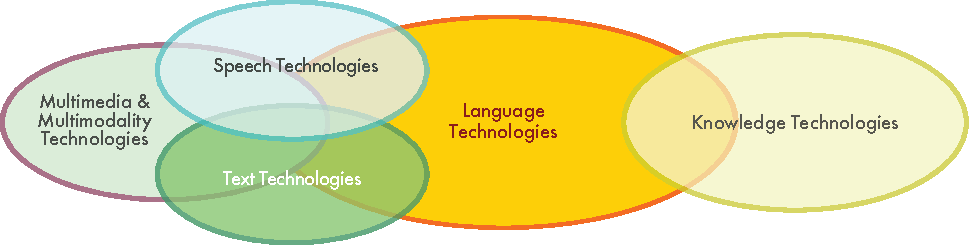
\includegraphics[width=\textwidth]{../_media/english/language_technologies}
  \caption{Language technology in context}
  \label{fig:ltincontext_en}
  \colorrule{grey3}{\textwidth}{1.5pt}
\end{figure*}

When we communicate, we combine language with other modes of communication and information media --- for example speaking can involve gestures and facial expressions. Digital texts link to pictures and sounds. Movies may contain language in spoken and written form. In other words, speech and text technologies overlap and interact with other multimodal communication and multimedia technologies.\\ 
In this section, we will discuss the main application areas of language technology, i.\,e., language checking, web search, speech interaction, and machine translation. These applications and basic technologies include 

\begin{itemize}
\item spelling correction
\item authoring support
\item computer-assisted language learning
\item information retrieval 
\item information extraction
\item text summarisation
\item question answering
\item speech recognition 
\item speech synthesis 
\end{itemize}

Language technology is an established area of research with an extensive set of introductory literature. The interested reader is referred to the following references:  \cite{carstensen-etal1, jurafsky-martin01, manning-schuetze1, lt-world1, lt-survey1}.

Before discussing the above application areas, we will briefly describe the architecture of a typical LT system.

\subsection{Application Architectures}

Software applications for language processing typically consist of several components that mirror different aspects of language. While such applications are typically very complex, figure~\ref{fig:textprocessingarch_en} shows a highly simplified architecture of a typical text processing system. The first three modules handle the structure and meaning of the text input:

\begin{enumerate}
\item Pre-processing: cleans the data, analyses or removes formatting, detects the input languages, and so on.
\item Grammatical analysis: finds the verb, its objects, modifiers and other parts of speech; detects the sentence structure.
\item Semantic analysis: performs disambiguation (i.\,e., computes the appropriate meaning of words in a given context); resolves anaphora (i.\,e., which pronouns refer to which nouns in the sentence); represents the meaning of the sentence in a machine-readable way.
\end{enumerate}

After analysing the text, task-specific modules can perform other operations, such as automatic summarisation and database look-ups.

In the remainder of this section, we firstly introduce the core application areas for language technology, and follow this with a brief overview of the state of LT research and education today, and a description of past and present research programmes. Finally, we present an expert estimate of core LT tools and resources for Estonian in terms of various dimensions such as availability, maturity and quality. The general situation of LT for the Estonian language is summarised in a matrix (figure~\ref{fig:lrlttable_en}). Tools and resources that are boldfaced in the text can also be found in figure~\ref{fig:lrlttable_en} (p.~\pageref{fig:lrlttable_en}) at the end of this chapter. LT support for Estonian is also compared to other languages that are part of this series.

\begin{figure*}[htb]
  \colorrule{grey3}{\textwidth}{1.5pt}
  \center
  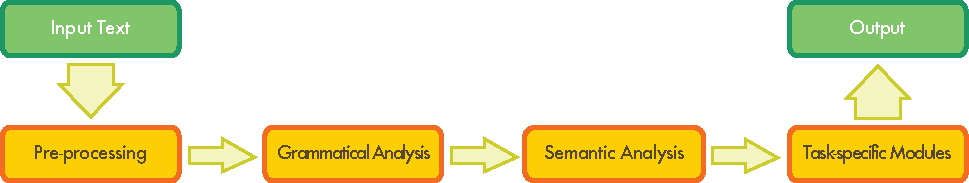
\includegraphics[width=\textwidth]{../_media/english/text_processing_app_architecture}
  \caption{A typical text processing architecture}
  \label{fig:textprocessingarch_en}
  \colorrule{grey3}{\textwidth}{1.5pt}
\end{figure*}

\subsection{Core Application Areas}

In this section, we focus on the most important LT tools and resources, and provide an overview of LT activities in Estonia. 

\subsubsection{Language Checking}

Anyone who has used a word processor such as Microsoft Word knows that it has a spell checker that highlights spelling mistakes and proposes corrections. The first spelling correction programs compared a list of extracted words against a dictionary of correctly spelled words. Today these programs are far more sophisticated. Using language-dependent algorithms for \textbf{grammatical analysis}, they detect errors related to morphology (e.\,g., plural formation) as well as syntax-related errors, such as a missing verb or a conflict of verb-subject agreement (e.\,g., \textit{she *write a letter}). However, most spell checkers will not find any errors in the following text \cite{zar1}:

\begin{quote}
  I have a spelling checker,\\
  It came with my PC.\\
  It plane lee marks four my revue\\
  Miss steaks aye can knot sea.
\end{quote}

Handling these kinds of errors usually requires an analysis of the context. For example: deciding whether the noun phrase has an agreement in case and number, as in:
\begin{quote}
 \textit {värvilise õied}\\ 
 colourful-SG-GEN blooms\\
 \textit {värvilise\textbf{d} õied}\\
 colourful-PL-NOM blooms
\end{quote}

This type of analysis either needs to draw on language-specific grammars laboriously coded into the software by experts, or on a statistical language model. 
In this case, a model calculates the probability of a particular word as it occurs in a specific position (e.g., between the words that precede and follow it). 
For example: \textit{värvilised õied} is a much more probable word sequence than \textit{värvilise õied}.
Language checking applications also automatically correct search engine queries, as found in Google's \textit{Did you mean…} suggestions.

A statistical language model can be automatically created by using a large amount of (correct) language data (called a text corpus). 
Most of these two approaches have been developed around data from English. 
Neither approach can transfer easily to Estonian because the language has a flexible word order, unlimited compound building and a richer inflection system. 

\begin{figure*}[htb]
  \colorrule{grey3}{\textwidth}{1.5pt}
  \center
  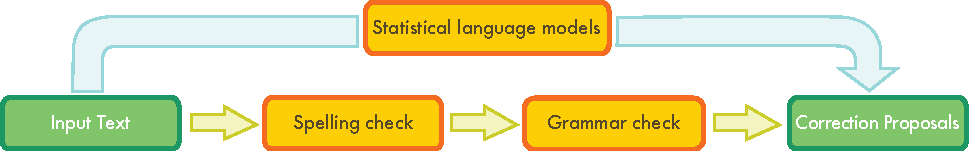
\includegraphics[width=\textwidth]{../_media/english/language_checking}
  \caption{Language checking (statistical; rule-based)}
  \label{fig:langcheckingaarch_en}
  \colorrule{grey3}{\textwidth}{1.5pt}
\end{figure*}

\boxtext{The use of language checking is not limited to word processors. It also applies to authoring support systems.}

The development of Estonian speller dates back to 1991. 
The implementation of speller software has been strongly related to the progress of development of morphological analyzer for Estonian, known under the name ESTMORF. 
The base for the speller and analyzer was the lexicon of 36,000 simple words and the descriptions for forming all word forms of them. 
The further development focused on the modeling of compounding and derivation.
In 1994, the first version of Estonian speller was released. 
The later versions have had better lexicons of proper names, abbreviations, neologisms etc.

The speller has been integrated with MS Office, OpenOffice.org and IBM Lotus Notes programs. The speller is being developed by the private company Filosoft \cite{Filosoft}.

Also, there have been other attempts for developing spellers for Estonian. 
Several versions of open source tools for spell-checking Estonian have been created. 
The lexicon for \textit{ispell} is most widely known. 
Its main disadvantage is the inability to handle compounds. 

Grammar checker verifies the structure and punctuation of the sentence. 
The development of Estonian grammar checker started in 2007 in the University of Tartu. 
At present time, a prototype of the checker has been created which is able to find places of missing commas with the precision of 95\%.

Language checking is not limited to word processors; it is also used
in ``authoring support systems'', i.\,e., software environments in
which manuals and other types of technical documentation for complex
IT, healthcare, engineering and other products, are written. To offset
customer complaints about incorrect use and damage claims resulting
from poorly understood instructions, companies are increasingly
focusing on the quality of technical documentation while targeting the
international market (via translation or localisation) at the same
time. Advances in natural language processing have led to the
development of authoring support software, which helps the writer of
technical documentation to use vocabulary and sentence structures that
are consistent with industry rules and (corporate) terminology
restrictions. 

Besides spell checkers and authoring support, language checking is also important in the field of computer-assisted language learning. 

\subsubsection{Web Search}

\begin{figure*}[htb]
  \colorrule{grey3}{\textwidth}{1.5pt}
  \center
  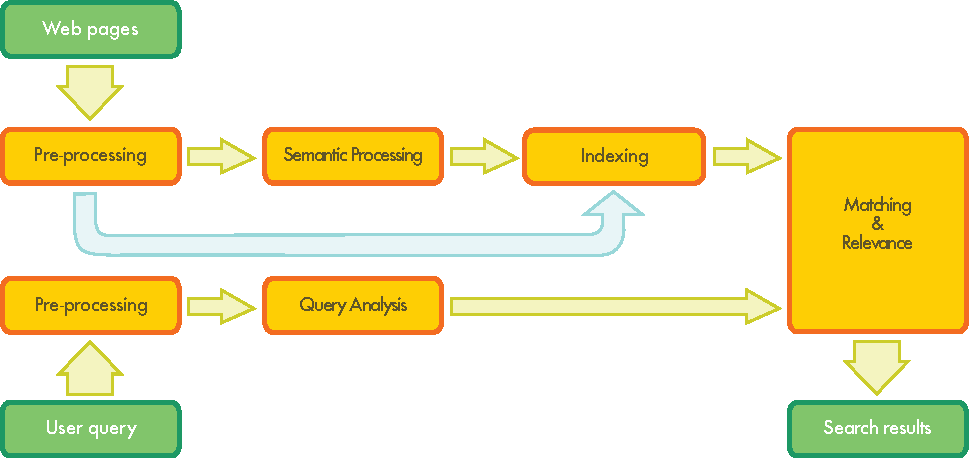
\includegraphics[width=\textwidth]{../_media/english/web_search_architecture}
  \caption{Web search}
  \label{fig:websearcharch_en}
  \colorrule{grey3}{\textwidth}{1.5pt}
 \end{figure*}

Searching the Web, intranets or digital libraries is probably the most widely used yet largely underdeveloped language technology application today. The Google search engine, which started in 1998, now handles about 80\% of all search queries \cite{spi1}. Since 2009, the verb \textit{guugeldama} has even had an entry in the Eesti Õigekeelsussõnaraamat (Estonian ortographic and explanatory dictionary). The Google search interface and results page display has not significantly changed since the first version. However, in the current version, Google offers spelling correction for misspelled words and incorporates basic semantic search capabilities that can improve search accuracy by analysing the meaning of terms in a search query context \cite{pc1}. The Google success story shows that a large volume of data and efficient indexing techniques can deliver satisfactory results using a statistical approach to language processing. 

For more sophisticated information requests, it is essential to integrate deeper linguistic knowledge to facilitate text interpretation. Experiments using \textbf{lexical resources} such as machine-readable thesauri or ontological language resources (e.\,g., WordNet for English or GermaNet for German) have demonstrated improvements in finding pages using synonyms of the original search terms, such as \textit{aatomienergia} {[}atomic energy{]} and \textit{tuumaenergia} {[}nuclear energy{]}, or even more loosely related terms.

\boxtext{The next generation of search engines will have to include much more sophisticated language technology.}

The next generation of search engines will have to include much more sophisticated language technology, escpecially to deal with search queries consisting of a question or other sentence type rather than a list of keywords. For the query, \textit{Give me a list of all companies that were taken over by other companies in the last five years}, a syntactic as well as \textbf{semantic analysis} is required. The system also needs to provide an index to quickly retrieve relevant documents. A satisfactory answer will require syntactic parsing to analyse the grammatical structure of the sentence and determine that the user wants companies that have been acquired, rather than companies that have acquired other companies. For the expression \textit{last five years}, the system needs to determine the relevant range of years, taking into account the present year. The query then needs to be matched against a huge amount of unstructured data to find the pieces of information that are relevant to the user’s request. This process is called information retrieval, and involves searching and ranking relevant documents. To generate a list of companies, the system also needs to recognise a particular string of words in a document represents a company name, using a process called named entity recognition.

A more demanding challenge is matching a query in one language with documents in another language. Cross-lingual information retrieval involves automatically translating the query into all possible source languages and then translating the results back into the user's target language.

Now that data is increasingly found in non-textual formats, there is a need for services that deliver multimedia information retrieval by searching images, audio files and video data. In the case of audio and video files, a speech recognition module must convert the speech content into text (or into a phonetic representation) that can then be matched against a user query.

Language independent search tools can only find the word forms which have the same form as the query word or include the query word as a substring. 
As Estonian is a language with rich morphology, and since in addition to the endings the stem itself may vary, the language specific tools are needed for searching and indexing. 

Documents are held in the computer as one big textual database. 
The problem of full text search is often divided into two sub-tasks: indexing and searching. 
The indexing stage will scan the texts of all documents and build a list of search terms, often called the index.
In the search stage, when performing a specific query, only the index is referenced rather than the text of the original documents.
The indexer will make an entry in the index for each term or word found in a document and possibly its relative position within the document. 
Language-specific indexers also employ language-specific stemming (lemmatising) on the words being indexed, so for example any token of the Estonian words \textit{käsi}, \textit{käe}, or \textit{kätt} (\textit{hand} in nominative, genitive and partitive case) will be recorded in the index under a single stem-form (lemma) \textit{käsi}.
In some cases, automatic lemmatiser may find many lemmas for one word form. 
For example, the lemmas of \textit{kuue} are \textit{kuub} (jacket) or \textit{kuus} (six). 
In order to solve this ambiguity, the system has to take account the context of the word and perform morphological disambiguation process.
 
It is officially recommended to use Estonian lemmatiser for searching and indexing of full-text databases in information systems of public sector in Estonia \cite{RIA}.
The first use of lemmatiser-based search was implemented 1997--2001 for information systems of State Chancellery.
Also Google search for Estonian includes some probably stochastic lemmatisation, e.g. search word \textit{majandusminister} would also return hits for \textit{majandusministri}, the singular genitive of \textit{majandusminister} (minister of economy).

\subsubsection{Speech Interaction}

Speech interaction is one of many application areas that depend on speech technology, i.\,e., technologies for processing spoken language. Speech interaction technology is used to create interfaces that enable users to interact in spoken language instead of using a graphical display, keyboard and mouse.  Today, these voice user interfaces (VUI) are used for partially or fully automated telephone services provided by companies to customers, employees or partners. Business domains that rely heavily on VUIs include banking, supply chain, public transportation, and telecommunications. Other uses of speech interaction technology include interfaces to car navigation systems and the use of spoken language as an alternative to the graphical or touchscreen interfaces in smartphones.

\begin{figure*}[htb]
  \colorrule{grey3}{\textwidth}{1.5pt}
  \center
  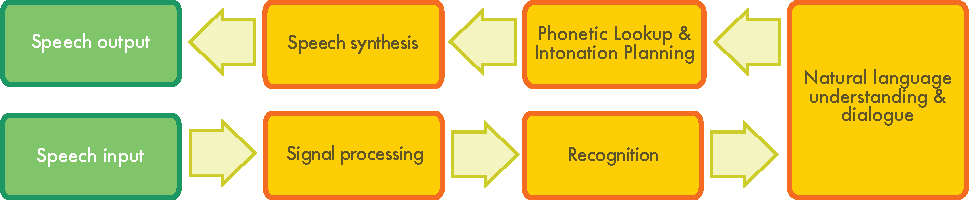
\includegraphics[width=\textwidth]{../_media/english/simple_speech-based_dialogue_architecture}
  \caption{Speech-based dialogue system}
  \label{fig:dialoguearch_en}
  \colorrule{grey3}{\textwidth}{1.5pt}
\end{figure*}

Speech interaction technology comprises four technologies: 

\begin{enumerate}
\item Automatic \textbf{speech recognition} (ASR) determines which words are actually spoken in a given sequence of sounds uttered by a user.  
\item Natural language understanding analyses the syntactic structure of a user’s utterance and interprets it according to the system in question.
\item Dialogue management determines which action to take given the user input and system functionality.   
\item \textbf{Speech synthesis} (text-to-speech or TTS) transforms the system’s reply into sounds for the user.
\end{enumerate}

One of the major challenges of ASR systems is to accurately recognise the words a user utters. This means restricting the range of possible user utterances to a limited set of keywords, or manually creating language models that cover a large range of natural language utterances. Using machine learning techniques, language models can also be generated automatically from \textbf{speech corpora}, i.\,e., large collections of speech audio files and text transcriptions. Restricting utterances usually forces people to use the voice user interface in a rigid way and can damage user acceptance; but the creation, tuning and maintenance of rich language models will significantly increase costs. VUIs that employ language models and initially allow a user to express their intent more flexibly — prompted by a \textit{How may I help you?} greeting — tend to be automated and are better accepted by users.

\boxtext{Speech interaction is the basis for creating interfaces that allow a user to interact with spoken language instead of a graphical display, keyboard and mouse.}

Companies tend to use pre-recorded utterances by professional speakers for generating the output of the voice user interface. For static utterances where the wording does not depend on particular contexts of use or personal user data, this can deliver a rich user experience. But more dynamic content in an utterance may suffer from unnatural intonation because bits of audio files have simply been strung together. Through optimisation, today’s TTS systems are getting better at producing natural-sounding dynamic utterances.

Interfaces in speech interaction have been considerably standardised during the last decade in terms of their various technological components. There has also been strong market consolidation in speech recognition and speech synthesis. The national markets in the G20 countries (economically resilient countries with high populations) have been dominated by just five global players, with Nuance (USA) and Loquendo (Italy) being the most prominent players in Europe. In 2011, Nuance announced the acquisition of Loquendo, which represents a further step in market consolidation.

During the last decade, the research on automatic speech recognition in Estonia has been carried out mainly at the Laboratory of Phonetics and Speech Technology, Institute of Cybernetics at Tallinn University of Technology (IOC). 
In 2000, a prototype for isolated word recognition (Estonian numbers and names of Estonian letters) was developed. In 2002--2004 a limited vocabulary connected speech recognition system based on hidden Markov models (HMM) as context-dependent phone units was developed. 
The last version (2010) of the system with unlimited vocabulary is able to recognize 63--85\% of words. 
The result depends heavily on the genre of the speech, vocabulary and the quality of the signal (the noise level) \cite{Phon}.

There is a web application of speech recognizer which enables to browse automatically transcribed conversational broadcasts, and both listen and search them. 
Also, a web service is available for users to send their own sound files to the system for the transcription. 
For more specific purposes, there is a speech recognition system for radiologists under development. 
The first experiments with it yielded promising results (only 10\% errors in real-time recognition).

During the years 1997--2002 the first Estonian text-to-speech synthesizer has been developed in the cooperation of IOC, Institute of Estonian Language (IEL) and Filosoft. 
It belongs to the first generation of speech synthesizers based on diphones. 
Every speech unit corresponds to exactly on diphone (sound-to-sound transition) in the database. 
The output of the synthesizer is understandable, but the sound itself is monotonous, with somewhat unnatural tone and poorly coherent. 
This synthesizer is adapted for use by blinds. 
The synthesizer is an open-source product, and may be used for non-commercial and non-military purposes \cite{IEL}. 

IEL is developing the new corpus-based version of the synthesizer where the longer speech units have been used in addition to diphones (word and phrase). 

The prize for the Best Language Deed in 2010 (established by the Ministry of Education and Research) was awarded to OÜ Jumalalaegas and the Estonian Library for the Blind for developing voice guidance tools for blinds. 
These tools use partially the speech synthesizer for Finnish.

Looking ahead, there will be significant changes, due to the spread of smartphones as a new platform for managing customer relationships, in addition to fixed telephones, the Internet and e-mail. This will also affect how speech interaction technology is used. In the long term, there will be fewer telephone-based VUIs, and spoken language apps will play a far more central role as a user-friendly input for smartphones. This will be largely driven by stepwise improvements in the accuracy of speaker-independent speech recognition via the speech dictation services already offered as centralised services to smartphone users. 

``Language recognition applications for smart phones'' by Tanel Alumäe
and Kaarel Kaljurand  developed at Institute of Cybernetics at TUT won
the grand prize of Language Deed 2011. 

\subsubsection{Machine Translation}

\begin{figure*}[htb]
  \colorrule{grey3}{\textwidth}{1.5pt}
  \center
  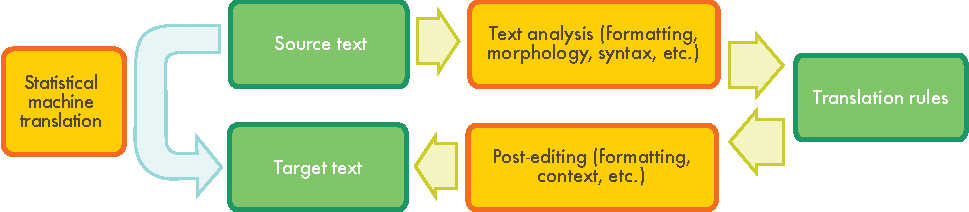
\includegraphics[width=\textwidth]{../_media/english/machine_translation}
  \caption{Machine translation (statistical; rule-based)}
  \label{fig:mtarch_en}
  \colorrule{grey3}{\textwidth}{1.5pt}
\end{figure*}

The idea of using digital computers to translate natural languages can be traced back to 1946 and was followed by substantial funding for research during the 1950s and again in the 1980s. 
Yet machine translation (MT) still cannot deliver on its initial promise of providing across-the-board automated translation.  

\boxtext{At its basic level, Machine Translation simply substitutes words in one natural language with words in another language.}

The most basic approach to machine translation is the automatic replacement of the words in a text written in one natural language with the equivalent words of another language. This can be useful in subject domains that have a very restricted, formulaic language such as weather reports.
However, in order to produce a good translation of less restricted texts, larger text units (phrases, sentences, or even whole passages) need to be matched to their closest counterparts in the target language. The major difficulty is that human language is ambiguous. Ambiguity creates challenges on multiple levels, such as word sense disambiguation on the lexical level (a \textit{mouse} is an input device of computer or an animal) or the assignment of case on the syntactic level, for example:

\begin{quote}
\textit{Naine nägi autot ja \textbf{mees} ka.}\\
\textit{Naine nägi autot ja \textbf{meest} ka.}\\
The woman saw the car and the man, too.
\end{quote}

One way to build an MT system is to use linguistic rules. For translations between closely related languages, a translation using direct substitution may be feasible in cases such as the above example. However, rule-based (or linguistic knowledge-driven) systems often analyse the input text and create an intermediary symbolic representation from which the target language text can be generated. The success of these methods is highly dependent on the availability of extensive lexicons with morphological, syntactic, and semantic information, and large sets of grammar rules carefully designed by skilled linguists. This is a very long and therefore costly process.

In the late 1980s when computational power increased and became cheaper, interest in statistical models for machine translation began to grow. Statistical models are derived from analysing bilingual text corpora, \textbf{parallel corpora}, such as the Europarl parallel corpus, which contains the proceedings of the European Parliament in 11 European languages. Given enough data, statistical MT works well enough to derive an approximate meaning of a foreign language text by processing parallel versions and finding plausible patterns of words. Unlike knowledge-driven systems, however, statistical (or data-driven) MT systems often generate ungrammatical output. Data-driven MT is advantageous because less human effort is required, and it can also cover special particularities of the language (e.\,g., idiomatic expressions) that are often ignored in knowledge-driven systems. 

The strengths and weaknesses of knowledge-driven and data-driven machine translation tend to be complementary, so that nowadays researchers focus on hybrid approaches that combine both methodologies. One such approach uses both knowledge-driven and data-driven systems, together with a selection module that decides on the best output for each sentence. However, results for sentences longer than, say, 12 words, will often be far from perfect. A more effective solution is to combine the best parts of each sentence from multiple outputs; this can be fairly complex, as corresponding parts of multiple alternatives are not always obvious and need to be aligned. 

\boxtext{Machine Translation is particularly challenging for the Estonian language.}

Machine translation is particularly challenging for the Estonian language. 
The potential for creating arbitrary new words by compounding makes dictionary analysis and dictionary coverage difficult; free word order and split verb constructions pose problems for analysis, also, the amount of available parallel texts is limited. 
In spite of this, Estonian belongs to one of the languages (currently, around 50) which can be translated by computer \cite{Koit}. 

The history of machine translation of Estonian dates back to the end of 50s when mathematicians of University of Tartu experimented with building a system for automatic translation of mathematical texts from Russian to Estonian. 
The hardware used during these experiments (computer Ural) had a speed of 100 operations per second, and this mediocre performance was one of the main reasons for discontinuing the experiments.

There exist two statistical machine translation systems for Estonian. 
The best known is the translation service by Google. 
Its quality is not always satisfactory but still enables the rough understanding of the text topic and basic facts.

The research group in the University of Tartu is currently working on the idea of Estonian-English machine translation. 
This translation system (located on the page masintolge.ut.ee) allows for the translation of sentences with a limited length from Estonian to English. 
This system uses open source SMT decoder Moses and is trained using JRC-Acquis, OPUS and other Estonian-English parallel corpora.

The use of machine translation can significantly increase productivity provided the system is intelligently adapted to user-specific terminology and integrated into a workflow. 
Special systems for interactive translation support were developed, for example, at Siemens. 
Language portals such as the Volkswagen site provide access to dictionaries, company-specific terminology, translation memory and MT support. 

There is still a huge potential for improving the quality of MT systems. The challenges involve adapting language resources to a given subject domain or user area, and integrating the technology into workflows that already have term bases and translation memories. Another problem is that most of the current systems are English-centred and only support a few languages from and into other European languages. This leads to friction in the translation workflow and forces MT users to learn different lexicon coding tools for different systems.

Evaluation campaigns help to compare the quality of MT systems, the different approaches and the status of the systems for different language pairs. Figure~\ref{fig:euromatrix_de} (p.~\pageref{fig:euromatrix_de}), which was prepared during the EC Euromatrix+ project, shows the pair-wise performances obtained for 22 of the 23 official EU languages (Irish was not compared). The results are ranked according to a BLEU score, which indicates higher scores for better translations \cite{bleu1}. A human translator would normally achieve a score of around 80 points.

The best results (in green and blue) were achieved by languages that benefit from a considerable research effort in coordinated programmes and the existence of many parallel corpora (e.\,g., English, French, Dutch, Spanish and German). The languages with poorer results are shown in red. These languages either lack such development efforts or are structurally very different from other languages (e.\,g., Hungarian, Maltese, Finnish and Estonian).

\subsection{Other Application Areas}

Building language technology applications involves a range of subtasks
that do not always surface at the level of interaction with the user,
but they provide significant service functionalities ``behind the
scenes'' of the system in question. They all form important research
issues that have now evolved into individual sub-disciplines of
computational linguistics.  Question answering, for example, is an
active area of research for which annotated corpora have been built
and scientific competitions have been initiated. The concept of
question answering goes beyond keyword-based searches (in which the
search engine responds by delivering a collection of potentially
relevant documents) and enables users to ask a concrete question to
which the system provides a single answer. For example: 

\begin{quote}
\textit{Question: How old was Neil Armstrong when he stepped on the moon?}\\
\textit{Answer: 38.}
\end{quote}

While question answering is obviously related to the core area of web search, it is nowadays an umbrella term for such research issues as which different types of questions exist, and how they should be handled; how a set of documents that potentially contain the answer can be analysed and compared (do they provide conflicting answers?); and how specific information (the answer) can be reliably extracted from a document without ignoring the context. 

\boxtext{Language technology applications often provide significant
  service functionalities `behind the scenes' of larger software
  systems.} 

Question answering is in turn related to information extraction (IE), an area that was extremely popular and influential when computational linguistics took a statistical turn in the early 1990s. IE aims to identify specific pieces of information in specific classes of documents, such as the key players in company takeovers as reported in newspaper stories. Another common scenario that has been studied is reports on terrorist incidents. The task here consists of mapping appropriate parts of the text to a template that specifies the perpetrator, target, time, location and results of the incident. Domain-specific template-filling is the central characteristic of IE, which makes it another example of a ``behind the scenes'' technology that forms a well-demarcated research area, which in practice needs to be embedded into a suitable application environment. 

    Text summarisation and \textbf{text generation} are two borderline areas that can act either as standalone applications or play a supporting role. Summarisation attempts to give the essentials of a long text in a short form, and is one of the features available in Microsoft Word. It mostly uses a statistical approach to identify the ``important'' words in a text (i.\,e., words that occur very frequently in the text in question but less frequently in general language use) and determine which sentences contain the most of these ``important'' words. These sentences are then extracted and put together to create the summary. In this very common commercial scenario, summarisation is simply a form of sentence extraction, and the text is reduced to a subset of its sentences. An alternative approach, for which some research has been carried out, is to generate brand new sentences that do not exist in the source text. 

This requires a deeper understanding of the text, which means that so far this approach is far less robust. On the whole, a text generator is rarely used as a stand-alone application but is embedded into a larger software environment, such as a clinical information system that collects, stores and processes patient data. Creating reports is just one of many applications for text summarisation. 

There exist only prototype versions of these tools for Estonian. 
The summarisation tool for Estonian (EstSum) focuses on extraction methods from a single document. 
The area of texts is limited: EstSum considers that the input text consists of a formatted news text. 

Question answering, information extraction, and summarisation have been the focus of numerous open competitions in the USA since the 1990s, primarily organised by the government-sponsored organisations DARPA and NIST. These competitions have significantly improved the state of the art, but their focus has mostly been on the English language. As a result, there are hardly any annotated corpora or other special resources for these tasks in Estonian. When summarisation systems use purely statistical methods, they are largely language-independent and a number of research prototypes are available. For text generation, reusable components have traditionally been limited to surface realisation modules (generation grammars) and most of the available software is for the English language. 

\subsection{Educational Programmes}

Language technology is a very interdisciplinary field that involves the combined expertise of linguists, computer scientists, mathematicians, philosophers, psycholinguists, and neuroscientists among others. 

Two universities in Estonia are involved in language technology education \cite{Meisteretal}: 
\begin{itemize}
 \item University of Tartu. Students of Estonian and Fenno-Ugric languages can study computer linguistics as a specialized module both during BSc and MSc program. The module includes various language theory and computer science courses, e.g., Programming for Linguists and Language Theory for Linguists. BSc and MSc students of Information Technology can study Language Technology as a specialized module. Many of these courses have been created jointly by the Department of Mathematics and Informatics and the Department of Philosophy. On the PhD level, the relevant research training is typically carried out under general linguistics or computer science.
\item  Tallinn University of Technology. Some PhD students of information technology are specializing in the field of speech technology, following individual study programs.
\end{itemize}

In 2009, two doctoral schools were established which involve PhD students of computer linguistics and language technology: the doctoral school of information and communication technology (includes students of language technology), and the doctoral school of language theory, philosophy and semiotics (includes students of computer linguistics).


\subsection{National Programmes and Initiatives}

The language technology was actively researched in Estonia already in 1950s when the first industrial grade computers appeared in universities and research labs. 
However, in the early 1990s the funding of many research activities changed considerably, with some research fields falling into extinction. 
HLT research groups survived quite well due to successful participation in several international projects (e.g. EU Copernicus) \cite{Meisteretal}.

Starting at the end of the 1990s, additional funding sources were opened: 
\begin{itemize}
 \item the Estonian Language Technology programme initiated by the Estonian Informatics Centre (1998--2000). Within this programme the first Development Plan for Estonian Language Technology was compiled in 1999;
 \item the national programmes ``Estonian Language and Cultural
   Heritage'' (1999--2003) and ``Estonian Language and National
   Memory'' (2004--2008) included sub-programmes for HLT. 
 \item HLT key-players were involved also in EU FP5 project ``eVikings II: Establishment of the Virtual Centre of Excellence for IST RTD in Estonia'' (2002--2005).
\end{itemize}

National Programme for Estonian Language Technology (NPELT) was compiled in 2005 by a group of HLT experts and launched by the Ministry of Education and Research in 2006 for a period of five years (2006--2010). 
The main goal of NPELT was to develop technology support for the Estonian language to the level that would allow functioning of Estonian in the modern information society. 
NPELT funded HLT-related R\&D activities including creation of reusable language resources and development of essential linguistic software (up to the working prototypes) as well as bringing the relevant language technology infrastructure up to date. 
The resources and prototypes funded by the national programme are publicly available \cite{ekktt}.

The Center of Estonian Language Resources (CELR) spun out of a project financed by NPELT. The aim of the Centre is to create an infrastructure to make available Estonian language resources and NLP software. By the end of 2011 a consortium was
formed by three partners: University of Tartu, the Institute of Cybernetics at Tallinn University of Technology and the Institute of the Estonian Language.

Continuing National Programme \cite{ekktt2} regarding the support of Estonian language technology is going on 2011--2017. 
This programme will focus more on applications and on making the developed resources and tools publicly available.

The Ministry of Education and Research is funding also more research-oriented projects on language technology using targeted financing schema and grants of Estonian Science Foundation.

The Center of Excellence of Computer Science (acting from 2008 to 2015) includes computational linguists from the University of Tartu and the Institute of Cybernetics of TTU (Tallinn University of Technology). 

Estonia has taken part in Common Language Resources and Technology
Infrastructure (CLARIN, see  \url{http://www.clarin.eu}) activities
since 2008. CLARIN legal form is ERIC (European Research
Infrastructure Consortium) from February 29, 2012. Center of Estonian
Language Resources as an object included in the Estonian Research
Infrastructures Roadmap will function as CLARIN centre of Estonia. 
  
\subsection{Availability of Tools and Resources}

Figure~\ref{fig:lrlttable_en} provides a rating for language technology support for the Estonian language. This rating of existing tools and resources was generated by leading experts in the field who provided estimates based on a scale from 0 (very low) to 6 (very high) using seven criteria.

\begin{figure*}[htb]
\centering
%\begin{tabular}{>{\columncolor{orange1}}p{.33\linewidth}ccccccc} % ORIGINAL
\begin{tabular}{>{\columncolor{orange1}}p{.33\linewidth}@{\hspace*{6mm}}c@{\hspace*{6mm}}c@{\hspace*{6mm}}c@{\hspace*{6mm}}c@{\hspace*{6mm}}c@{\hspace*{6mm}}c@{\hspace*{6mm}}c}
\rowcolor{orange1}
 \cellcolor{white}&\begin{sideways}\makecell[l]{Quantity}\end{sideways}
&\begin{sideways}\makecell[l]{\makecell[l]{Availability} }\end{sideways} &\begin{sideways}\makecell[l]{Quality}\end{sideways}
&\begin{sideways}\makecell[l]{Coverage}\end{sideways} &\begin{sideways}\makecell[l]{Maturity}\end{sideways} &\begin{sideways}\makecell[l]{Sustainability}\end{sideways} &\begin{sideways}\makecell[l]{Adaptability}\end{sideways} \\ \addlinespace
\multicolumn{8}{>{\columncolor{orange2}}l}{Language Technology: Tools, Technologies and Applications} \\ \addlinespace
Speech Recognition	&2&5&2.8&2.8&3&3&3 \\ \addlinespace
Speech Synthesis &2&5&2.8&2.8&3&2&3\\ \addlinespace
Grammatical analysis &2.5&3.5&3.2&2.8&4&2.5&3.5 \\ \addlinespace
Semantic analysis &1&1.3&0.9&0.9&1.3&1.3&1.7 \\ \addlinespace
Text generation &0&0&0&0&0&0&0\\ \addlinespace
Machine translation &3&3&1.4&2.1&3&4&2 \\ \addlinespace
\multicolumn{8}{>{\columncolor{orange2}}l}{Language Resources: Resources, Data and Knowledge Bases} \\ \addlinespace
Text corpora &3&5&2.5&2.1&3&2.5 \\ \addlinespace
Speech corpora &2&5&2.1&2.8&4&4&4 \\ \addlinespace
Parallel corpora &2&2&2.1&1.4&3&3&2 \\ \addlinespace
Lexical resources &3.5&4&3.2&2.8&3.5&3.5&3.5 \\ \addlinespace
Grammars &2&5&2.8&2.8&3&3&3\\
\end{tabular}
\caption{State of language technology support for Estonian}
\label{fig:lrlttable_en}
\end{figure*}

The key results for Estonian language technology can be summed up as follows:

\begin{itemize}
\item Tools for speech recognition and speech synthesis have been developed by research institutions; however these tools can be regarded as prototypes, not as mature products.
\item Although the automatic morphological analysis of Estonian is complicated, the efficiency of morphological tools (such as tokenizer, lemmatizer and morphological analyzer) is comparable to similar tools for other major European languages. Since the tools have been developed as commercial products, their licensing conditions have not allowed for unrestricted use by general public. On the other hand, the quality of publicly available tools has remained fairly modest, therefore the public preference has settled for commercial utilities.
Syntactic parsers with a broad coverage of Estonian have been developed only using one rule-based grammatical formalism. The grammar of the parser has been adapted for different genres of language. Nevertheless, the development of these tools must continue for achieving better performance.
Semantics is more difficult to process than syntax, and text semantics is more difficult to process than word and sentence semantics. 
Semantic tools and resources are scored low. 
Thus, programs and initiatives are needed to substantially boost this area both with regard to basic research and the development of annotated corpora.
\item Programs for text interpretation require extensive semantic analysis and these programs are only in the initial state of development. 
\item The only available tool for Estonian text generation is morphological synthesiser.
\item Most of the users prefer Google machine translation service. Also, Estonian-English machine translation system is under development in the University of Tartu. There would probably be a high demand for the Russian-Estonian and Estonian-Russian automatic translation service.
\item With regard to resources such as reference corpora, lexicons, wordnets and terminologies, the situation is also reasonably good for Estonian since substantial resources have been built in recent decades. While some reference corpora of high quality exist, syntactically and semantically annotated corpora are small in size. The work on multimodal corpora has begun recently.
\item Research was successful in designing particular high quality software, but many of the resources lack standardization and detail documentation, i.e., even if they exist, sustainability is not given; concerted programs and initiatives are needed to standardize data and interchange formats.

\end{itemize}

To sum up, the results indicate that Estonian stands reasonably well with respect to the most basic language technology tools and resources, such as tokenizers, PoS taggers, morphological analyzers, shallow parsers, reference corpora, treebanks and tools for speech technology. Furthermore, there exist some tools for summarization, machine translation, as well as resources like parallel corpora, and specialized corpora. However, these tools and resources are rather simple and have a limited functionality for some of the areas. For instance, parallel corpora only exist for very few language pairs and for limited text genres.
When it comes to more advanced fields like text semantics, language generation, and annotated multimodal data, Estonian clearly lacks basic tools and resources even if some of these are currently under development. 
The research regarding the most advanced tools and resources like discourse processing, dialogue management, semantics and discourse corpora has yielded first results but the resources need still to complement in amount and quality and tools have a quite limited scope.
Most of these tools (except morphological analyzer) have been developed by research institutions and can be regarded as prototypes, not as mature products. The development was supported by different national programmes of language technology what guarantees the availability of these tools.

\subsection{Cross-language comparison}

\begin{figure*}[tb]
  \small
  \centering
  \begin{tabular}
  { % defines color for each column.
  >{\columncolor{corange5}}p{.13\linewidth}@{\hspace{.040\linewidth}}
  >{\columncolor{corange4}}p{.13\linewidth}@{\hspace{.040\linewidth}}
  >{\columncolor{corange3}}p{.13\linewidth}@{\hspace{.040\linewidth}}
  >{\columncolor{corange2}}p{.13\linewidth}@{\hspace{.040\linewidth}}
  >{\columncolor{corange1}}p{.13\linewidth} 
  }
  \multicolumn{1}{>{\columncolor{white}}c@{\hspace{.040\linewidth}}}{\textbf{Excellent}} & 
  \multicolumn{1}{@{}>{\columncolor{white}}c@{\hspace{.040\linewidth}}}{\textbf{Good}} &
  \multicolumn{1}{@{}>{\columncolor{white}}c@{\hspace{.040\linewidth}}}{\textbf{Moderate}} &
  \multicolumn{1}{@{}>{\columncolor{white}}c@{\hspace{.040\linewidth}}}{\textbf{Fragmentary}} &
  \multicolumn{1}{@{}>{\columncolor{white}}c}{\textbf{Weak/no}} \\ 
  \multicolumn{1}{>{\columncolor{white}}c@{\hspace{.040\linewidth}}}{\textbf{support}} & 
  \multicolumn{1}{@{}>{\columncolor{white}}c@{\hspace{.040\linewidth}}}{\textbf{support}} &
  \multicolumn{1}{@{}>{\columncolor{white}}c@{\hspace{.040\linewidth}}}{\textbf{support}} &
  \multicolumn{1}{@{}>{\columncolor{white}}c@{\hspace{.040\linewidth}}}{\textbf{support}} &
  \multicolumn{1}{@{}>{\columncolor{white}}c}{\textbf{support}} \\ \addlinespace
  
& \vspace*{0.5mm}English
& \vspace*{0.5mm}
Czech \newline 
Dutch \newline 
Finnish \newline 
French \newline 
German \newline   
Italian \newline  
Portuguese \newline 
Spanish \newline
& \vspace*{0.5mm}Basque \newline 
Bulgarian \newline 
Catalan \newline 
Danish \newline 
Estonian \newline 
Galician\newline 
Greek \newline  
Hungarian  \newline
Irish \newline  
Norwegian \newline 
Polish \newline 
Serbian \newline 
Slovak \newline 
Slovene \newline 
Swedish \newline
& \vspace*{0.5mm}
Croatian \newline 
Icelandic \newline  
Latvian \newline 
Lithuanian \newline 
Maltese \newline 
Romanian\\
\end{tabular}
\caption{Speech processing: state of language technology support for 30 European languages}
\label{fig:speech_cluster_en}
\end{figure*}

\begin{figure*}[tb]
  \small
  \centering
  \begin{tabular}
  { % defines color for each column.
  >{\columncolor{corange5}}p{.13\linewidth}@{\hspace{.040\linewidth}}
  >{\columncolor{corange4}}p{.13\linewidth}@{\hspace{.040\linewidth}}
  >{\columncolor{corange3}}p{.13\linewidth}@{\hspace{.040\linewidth}}
  >{\columncolor{corange2}}p{.13\linewidth}@{\hspace{.040\linewidth}}
  >{\columncolor{corange1}}p{.13\linewidth} 
  }
  \multicolumn{1}{>{\columncolor{white}}c@{\hspace{.040\linewidth}}}{\textbf{Excellent}} & 
  \multicolumn{1}{@{}>{\columncolor{white}}c@{\hspace{.040\linewidth}}}{\textbf{Good}} &
  \multicolumn{1}{@{}>{\columncolor{white}}c@{\hspace{.040\linewidth}}}{\textbf{Moderate}} &
  \multicolumn{1}{@{}>{\columncolor{white}}c@{\hspace{.040\linewidth}}}{\textbf{Fragmentary}} &
  \multicolumn{1}{@{}>{\columncolor{white}}c}{\textbf{Weak/no}} \\ 
  \multicolumn{1}{>{\columncolor{white}}c@{\hspace{.040\linewidth}}}{\textbf{support}} & 
  \multicolumn{1}{@{}>{\columncolor{white}}c@{\hspace{.040\linewidth}}}{\textbf{support}} &
  \multicolumn{1}{@{}>{\columncolor{white}}c@{\hspace{.040\linewidth}}}{\textbf{support}} &
  \multicolumn{1}{@{}>{\columncolor{white}}c@{\hspace{.040\linewidth}}}{\textbf{support}} &
  \multicolumn{1}{@{}>{\columncolor{white}}c}{\textbf{support}} \\ \addlinespace
  
& \vspace*{0.5mm} English 
& \vspace*{0.5mm} 
French \newline 
Spanish
& \vspace*{0.5mm}
Catalan \newline 
Dutch \newline 
German \newline 
Hungarian \newline
Italian \newline 
Polish \newline 
Romanian \newline 
& \vspace*{0.5mm}Basque \newline 
Bulgarian \newline 
Croatian \newline 
Czech \newline
Danish \newline 
Estonian \newline 
Finnish \newline 
Galician \newline 
Greek \newline 
Icelandic \newline 
Irish \newline 
Latvian \newline 
Lithuanian \newline 
Maltese \newline 
Norwegian \newline 
Portuguese \newline 
Serbian \newline 
Slovak \newline 
Slovene \newline 
Swedish \newline 
\end{tabular}
\caption{Machine translation: state of language technology support for 30 European languages}
\label{fig:mt_cluster_en}
\end{figure*}

\begin{figure*}[tb]
  \small
  \centering
  \begin{tabular}
  { % defines color for each column.
  >{\columncolor{corange5}}p{.13\linewidth}@{\hspace{.040\linewidth}}
  >{\columncolor{corange4}}p{.13\linewidth}@{\hspace{.040\linewidth}}
  >{\columncolor{corange3}}p{.13\linewidth}@{\hspace{.040\linewidth}}
  >{\columncolor{corange2}}p{.13\linewidth}@{\hspace{.040\linewidth}}
  >{\columncolor{corange1}}p{.13\linewidth} 
  }
  \multicolumn{1}{>{\columncolor{white}}c@{\hspace{.040\linewidth}}}{\textbf{Excellent}} & 
  \multicolumn{1}{@{}>{\columncolor{white}}c@{\hspace{.040\linewidth}}}{\textbf{Good}} &
  \multicolumn{1}{@{}>{\columncolor{white}}c@{\hspace{.040\linewidth}}}{\textbf{Moderate}} &
  \multicolumn{1}{@{}>{\columncolor{white}}c@{\hspace{.040\linewidth}}}{\textbf{Fragmentary}} &
  \multicolumn{1}{@{}>{\columncolor{white}}c}{\textbf{Weak/no}} \\ 
  \multicolumn{1}{>{\columncolor{white}}c@{\hspace{.040\linewidth}}}{\textbf{support}} & 
  \multicolumn{1}{@{}>{\columncolor{white}}c@{\hspace{.040\linewidth}}}{\textbf{support}} &
  \multicolumn{1}{@{}>{\columncolor{white}}c@{\hspace{.040\linewidth}}}{\textbf{support}} &
  \multicolumn{1}{@{}>{\columncolor{white}}c@{\hspace{.040\linewidth}}}{\textbf{support}} &
  \multicolumn{1}{@{}>{\columncolor{white}}c}{\textbf{support}} \\ \addlinespace

& \vspace*{0.5mm}English
& \vspace*{0.5mm}
  Dutch \newline 
  French \newline 
  German \newline 
  Italian \newline 
  Spanish
& \vspace*{0.5mm}Basque \newline 
  Bulgarian \newline 
  Catalan \newline 
  Czech \newline 
  Danish \newline 
  Finnish \newline 
  Galician \newline 
  Greek \newline 
  Hungarian \newline 
  Norwegian \newline 
  Polish \newline 
  Portuguese \newline 
  Romanian \newline 
  Slovak \newline 
  Slovene \newline 
  Swedish \newline 
& \vspace*{0.5mm}
  Croatian \newline 
  Estonian \newline 
  Icelandic \newline 
  Irish \newline 
  Latvian \newline 
  Lithuanian \newline 
  Maltese \newline 
  Serbian \\
  \end{tabular}
\caption{Text analysis: state of language technology support for 30 European languages}
\label{fig:text_cluster_en}
\end{figure*}

\begin{figure*}[tb]
  \small
  \centering
  \begin{tabular}
  { % defines color for each column.
  >{\columncolor{corange5}}p{.13\linewidth}@{\hspace{.040\linewidth}}
  >{\columncolor{corange4}}p{.13\linewidth}@{\hspace{.040\linewidth}}
  >{\columncolor{corange3}}p{.13\linewidth}@{\hspace{.040\linewidth}}
  >{\columncolor{corange2}}p{.13\linewidth}@{\hspace{.040\linewidth}}
  >{\columncolor{corange1}}p{.13\linewidth} 
  }
  \multicolumn{1}{>{\columncolor{white}}c@{\hspace{.040\linewidth}}}{\textbf{Excellent}} & 
  \multicolumn{1}{@{}>{\columncolor{white}}c@{\hspace{.040\linewidth}}}{\textbf{Good}} &
  \multicolumn{1}{@{}>{\columncolor{white}}c@{\hspace{.040\linewidth}}}{\textbf{Moderate}} &
  \multicolumn{1}{@{}>{\columncolor{white}}c@{\hspace{.040\linewidth}}}{\textbf{Fragmentary}} &
  \multicolumn{1}{@{}>{\columncolor{white}}c}{\textbf{Weak/no}} \\ 
  \multicolumn{1}{>{\columncolor{white}}c@{\hspace{.040\linewidth}}}{\textbf{support}} & 
  \multicolumn{1}{@{}>{\columncolor{white}}c@{\hspace{.040\linewidth}}}{\textbf{support}} &
  \multicolumn{1}{@{}>{\columncolor{white}}c@{\hspace{.040\linewidth}}}{\textbf{support}} &
  \multicolumn{1}{@{}>{\columncolor{white}}c@{\hspace{.040\linewidth}}}{\textbf{support}} &
  \multicolumn{1}{@{}>{\columncolor{white}}c}{\textbf{support}} \\ \addlinespace
    
& \vspace*{0.5mm}English
& \vspace*{0.5mm} 
    Czech \newline 
    Dutch \newline 
    French \newline 
    German \newline 
    Hungarian \newline
    Italian \newline
    Polish \newline
    Spanish \newline
    Swedish \newline 
& \vspace*{0.5mm} Basque\newline 
    Bulgarian\newline 
    Catalan \newline 
    Croatian \newline 
    Danish \newline 
    Estonian \newline 
    Finnish \newline 
    Galician \newline 
    Greek \newline 
    Norwegian \newline 
    Portuguese \newline 
    Romanian \newline 
    Serbian \newline 
    Slovak \newline 
    Slovene \newline
&  \vspace*{0.5mm}
    Icelandic \newline 
    Irish \newline 
    Latvian \newline 
    Lithuanian \newline 
    Maltese  \\
  \end{tabular}
  \caption{Speech and text resources: State of support for 30 European languages}  
  \label{fig:resources_cluster_en}
\end{figure*}

The current state of LT support varies considerably from one language community to another. In order to compare the situation between languages, this section will present an evaluation based on two sample application areas (machine translation and speech processing) and one underlying technology (text analysis), as well as basic resources needed for building LT applications. The languages were categorised using the following five-point scale: 

\begin{enumerate}
\item Excellent support
\item Good support
\item Moderate support
\item Fragmentary support
\item Weak or no support
\end{enumerate}

LT support was measured according to the following criteria:

\textbf{Speech Processing:} Quality of existing speech recognition technologies, quality of existing speech synthesis technologies, coverage of domains, number and size of existing speech corpora, amount and variety of available speech-based applications.

\textbf{Machine Translation:} Quality of existing MT technologies, number of language pairs covered, coverage of linguistic phenomena and domains, quality and size of existing parallel corpora, amount and variety of available MT applications.

\textbf{Text Analysis:} Quality and coverage of existing text analysis technologies (morphology, syntax, semantics), coverage of linguistic phenomena and domains, amount and variety of available applications, quality and size of existing (annotated) text corpora, quality and coverage of existing lexical resources (e.\,g., WordNet) and grammars.

\textbf{Resources:} Quality and size of existing text corpora, speech corpora and parallel corpora, quality and coverage of existing lexical resources and grammars.

Figures \ref{fig:speech_cluster_en} to~\ref{fig:resources_cluster_en} show that, although the government has increased the support to the Estonian LT recent years, Estonian language belongs to the fourth or fifth clusters. 
The results of Estonian and Finnish are quite similar and Estonian is slightly better equipped than most other languages with a similar number of speakers, such as Latvian, Lithuanian, Icelandic and Maltese. 

All these languages lag far behind large languages like German and French, for instance. 
But even LT resources and tools for those languages clearly do not yet reach the quality and coverage of comparable resources and tools for the English language, which is in the lead in almost all LT areas. 
And there are still plenty of gaps in English language resources with regard to high quality applications

However, for building more sophisticated applications, such as machine translation, there is a clear need for resources and technologies that cover a wider range of linguistic aspects and allow a deep semantic analysis of the input text. 
By improving the quality and coverage of these basic resources and technologies, we shall be able to open up new opportunities for tackling a vast range of advanced application areas, including high-quality machine translation.


\subsection{Conclusions}

\emph{In this series of white papers, we have made an important effort by assessing the language technology support for 30 European languages, and by providing a high-level comparison across these languages. By identifying the gaps, needs and deficits, the European language technology community and its related stakeholders are now in a position to design a large scale research and development programme aimed at building a truly multilingual, technology-enabled communication across Europe.}

The results of this white paper series show that there is a dramatic difference in language technology support for the various European languages. While there are good quality software and resources available for some languages and application areas, others, usually smaller languages, have substantial gaps. Many languages lack basic technologies for text analysis and the essential resources. Others have basic tools and resources but the implementation of for example semantic methods is still far away. Therefore a large-scale effort is needed to attain the ambitious goal of providing high-quality language technology support for all European languages, for example through high quality machine translation. 

In the case of the Estonian language, we can be cautiously optimistic about the current state of language technology support. Supported by larger research programs in the past, there exists a language technology research scene in Estonia. Unfortunately, the industry consists only of a few SMEs.

For Estonian, a number of technologies and resources exist, but far less than for English. 
Language technology support today is by far not in a state that is needed for offering the support a true multilingual knowledge society needs.

The need for large amounts of data and the extreme complexity of language technology systems makes it vital to develop a new infrastructure and a more coherent research organization to spur greater sharing and cooperation.

Finally there is a lack of continuity in research and development funding. Short-term coordinated programmes tend to alternate with periods of sparse or zero funding. In addition, there is an overall lack of coordination with programmes in other EU countries and at the European Commission level.

The long term goal of META-NET is to enable the creation of high-quality language technology for all languages. This requires all stakeholders - in politics, research, business, and society - to unite their efforts. The resulting technology will help tear down existing barriers and build bridges between Europe’s languages, paving the way for political and economic unity through cultural diversity. 
\end{multicols}

\clearpage

\ssection[About META-NET]{About META-NET}

\begin{multicols}{2}

\textbf{META-NET} is a Network of Excellence funded by the European Commission. The network currently consists of 54 members from 33 European countries. 
META-NET forges \textbf{META}, the Multilingual Europe Technology Alliance, a growing community of language technology professionals and organisations in Europe.
META-NET fosters the technological foundations for a truly multilingual European information society that:

\begin{itemize}
\item makes communication and cooperation possible across languages;
\item grants all Europeans equal access to information and knowledge regardless of their language;
\item builds upon and advances functionalities of networked information technology.
\end{itemize}

The network supports a Europe that unites as a single digital market and information space. It stimulates and promotes multilingual technologies for all European languages. These technologies support automatic translation, content production, information processing and knowledge management for a wide variety of subject domains and applications. They also enable intuitive language-based interfaces to technology ranging from household electronics, machinery and vehicles to computers and robots.

Launched on 1 February 2010, META-NET has already conducted various activities in its three lines of action META-VISION, META-SHARE and META-RESEARCH. 

\textbf{META-VISION} fosters a dynamic and influential stakeholder community that unites around a shared vision and a common strategic research agenda (SRA). The main focus of this activity is to build a coherent and cohesive LT community in Europe by bringing together representatives from highly fragmented and diverse groups of stakeholders. The present White Paper was prepared together with volumes for 29 other languages. The shared technology vision was developed in three sectorial Vision Groups. The META Technology Council was established in order to discuss and to prepare the SRA based on the vision in close interaction with the entire LT community.

\textbf{META-SHARE} creates an open, distributed facility for exchanging and sharing resources. The peer-to-peer network of repositories will contain language data, tools and web services that are documented with high-quality metadata and organised in standardised categories. The resources can be readily accessed and uniformly searched. The available resources include free, open source materials as well as restricted, commercially available, fee-based items. 

\textbf{META-RESEARCH} builds bridges to related technology fields. This activity seeks to leverage advances in other fields and to capitalise on innovative research that can benefit language technology. In particular, the action line focuses on conducting leading-edge research in machine translation, collecting data, preparing data sets and organising language re-sources for evaluation purposes; compiling inventories of tools and methods; and organising workshops and training events for members of the community.

\end{multicols}

\cleardoublepage

\appendix
\addtocontents{toc}{\protect\bigskip}

\bsection[Kirjandus --- References]{Kirjandus --- References}
\bibliographystyle{unsrt}
\bibliography{estonian_references}
  
\cleardoublepage

\bsection[META-NETi liikmed -- META-NET Members]{META-NETi liikmed --- META-NET Members}
\label{metanetmembers}

\small
\begin{longtable}{llp{105mm}}
  Austria & \textcolor{grey1}{Austria} & Zentrum für Translationswissenschaft, Universität Wien: Gerhard Budin\\ \addlinespace 
  Belgia & \textcolor{grey1}{Belgium} & Computational Linguistics and Psycholinguistics Research Centre, Univ. of Antwerp: Walter Daelemans\\ \addlinespace
  & & Centre for Proc. Speech and Images, Univ. of Leuven: Dirk van Compernolle \\ \addlinespace
  Bulgaaria & \textcolor{grey1}{Bulgaria} & Inst. for Bulgarian Lang., Bulgarian Academy of Sciences: Svetla Koeva \\ \addlinespace
  Eesti & \textcolor{grey1}{Estonia} & Inst. of Computer Science, Univ. of Tartu: Kadri Vider\\ \addlinespace
  Hispaania & \textcolor{grey1}{Spain} & Barcelona Media: Toni Badia \\ \addlinespace 
  & & Institut Universitari de Lingüistica Aplicada, Univ. Pompeu Fabra: Núria Bel \\ \addlinespace 
  & & Aholab Signal Proc. Lab., Univ. of the Basque Country: Inma Hernaez Rioja \\ \addlinespace 
  & & Center for Lang. and Speech Technologies and Applications, Technical Univ. of Catalonia: Asunción Moreno \\ \addlinespace 
  & & Dept. of Signal Proc. and Communications, Univ. of Vigo: Carmen García Mateo \\ \addlinespace 
  & & Computational Linguistics, Univ. of Groningen: Gertjan van Noord\\ \addlinespace
  Horvaatia & \textcolor{grey1}{Croatia} & Inst. of Linguistics, Faculty of Humanities and Social Science, Univ. of Zagreb: Marko Tadić \\ \addlinespace
  Iirimaa & \textcolor{grey1}{Ireland} & School of Computing, Dublin City Univ.: Josef van Genabith\\ 
\addlinespace Iisrael & \textcolor{grey1}{Israel} & Dept. of Computer Sciences, Bar-Ilan University: Ido Dagan \\
\addlinespace  
  Island & \textcolor{grey1}{Iceland} & School of Humanities, Univ. of Iceland: Eirikur Rögnvaldsson\\ \addlinespace
  Itaalia & \textcolor{grey1}{Italy} & Consiglio Nazionale Ricerche, Istituto di Linguistica Computazionale ``Antonio Zampolli'': Nicoletta Calzolari\\ \addlinespace
  & & Human Lang. Technology, Fondazione Bruno Kessler: Bernardo Magnini\\ \addlinespace 
  Kreeka & \textcolor{grey1}{Greece} & Inst. for Lang. and Speech Proc., R.C. ``Athena'': Stelios Piperidis\\ \addlinespace
  Küpros & \textcolor{grey1}{Cyprus} & Lang. Centre, School of Humanities: Jack Burston\\ \addlinespace
  Leedu & \textcolor{grey1}{Lithuania} & Inst. of the Lithuanian Lang.: Jolanta Zabarskaitė\\ \addlinespace
  Läti & \textcolor{grey1}{Latvia} & Tilde: Andrejs Vasiljevs\\ \addlinespace 
  & & Inst. of Mathematics and Computer Science, Univ. of Latvia: Inguna Skadina\\ 
\addlinespace
  Luksemburg & \textcolor{grey1}{Luxembourg} & Arax Ltd.: Vartkes Goetcherian\\
\addlinespace 
  Madalmaad & \textcolor{grey1}{Netherlands} & Utrecht Inst. of Linguistics, Utrecht Univ.: Jan Odijk\\ 
 \addlinespace
  Malta & \textcolor{grey1}{Malta} & Dept. Intelligent Computer Systems, Univ. of Malta: Mike Rosner\\ \addlinespace
  Norra & \textcolor{grey1}{Norway} & Dept. of Linguistic, Univ. of Bergen: Koenraad De Smedt\\ \addlinespace 
  & & Dept. of Informatics, Lang. Technology Group, Univ. of Oslo: Stephan Oepen \\ \addlinespace
  Poola & \textcolor{grey1}{Poland} & Inst. of Computer Science, Polish Academy of Sciences: Adam Przepiórkowski, Maciej Ogrodniczuk \\ \addlinespace
  & & Univ. of Łódź: Barbara Lewandowska-Tomaszczyk, Piotr Pęzik\\ \addlinespace
  & & Dept. of Computer Linguistics and Artificial Intelligence, Adam Mickiewicz Univ.: Zygmunt Vetulani \\ \addlinespace
  Portugal & \textcolor{grey1}{Portugal} & Dept. of Informatics, Univ. of Lisbon: Antonio Branco\\ \addlinespace
  & & Spoken Lang. Systems Lab., Inst. for Systems Engineering and Computers: Isabel Trancoso \\ \addlinespace
  Prantsusmaa & \textcolor{grey1}{France} & Centre National de la Recherche Scientifique, Laboratoire d'Informatique pour la Mécanique et les Sciences de l'Ingénieur: Joseph Mariani \\ \addlinespace
  & & Evaluations and Lang. Resources Distribution Agency: Khalid Choukri\\ \addlinespace 
  Rootsi & \textcolor{grey1}{Sweden} & Dept. of Swedish Lang., Univ. of Gothenburg: Lars Borin \\ \addlinespace 
  Rumeenia & \textcolor{grey1}{Romania} & Research Inst. for Artificial Intelligence, Romanian Academy of Sciences: Dan Tufis \\ \addlinespace
  & & Faculty of Computer Science, Univ. Alexandru Ioan Cuza: Dan Cristea \\ \addlinespace
  Saksamaa & \textcolor{grey1}{Germany} & DFKI (German Research Centre for Artificial Intelligence): Hans Uszkoreit, Georg Rehm\\ \addlinespace
  & & Human Lang. Technology and Pattern Recognition, RWTH Aachen Univ.: Hermann Ney \\ \addlinespace
  & & Dept. of Computational Linguistics, Saarland Univ.: Manfred Pinkal\\ 
 \addlinespace  
  Serbia & \textcolor{grey1}{Serbia} & Faculty of Mathematics, Belgrade Univ.: Dusko Vitas, Cvetana Krstev, Ivan Obradovic \\ \addlinespace
  & & Pupin Inst.: Sanja Vranes \\ \addlinespace  
  Slovakkia & \textcolor{grey1}{Slovakia} & Ludovit Stur Inst. of Linguistics, Slovak Academy of Sciences: Radovan Garabik \\ \addlinespace 
  Sloveenia & \textcolor{grey1}{Slovenia} & Jozef Stefan Inst.: Marko Grobelnik \\ \addlinespace 
  Soome & \textcolor{grey1}{Finland} & Computational Cognitive Systems Research Group, Aalto Univ.: Timo Honkela\\ \addlinespace
  & & Dept. of Modern Languages, Univ. of Helsinki: Kimmo Koskenniemi, Krister Lindén \\ \addlinespace
  Suurbritannia & \textcolor{grey1}{United Kingdom} & Inst. for Lang., Cognition and Computation, Center for Speech Technology Research, Univ. of Edinburgh: Steve Renals \\ \addlinespace 
  & & Research Inst. of Informatics and Lang. Proc., Univ. of Wolverhampton: Ruslan Mitkov \\ \addlinespace 
  & & School of Computer Science, Univ. of Manchester: Sophia Ananiandou \\ \addlinespace 
  Šveits & \textcolor{grey1}{Switzerland} & Idiap Research Inst.: Hervé Bourlard \\ 
\addlinespace Taani &  \textcolor{grey1}{Denmark} & Centre for Lang. Technology, Univ. of Copenhagen: Bolette Sandford Pedersen, Bente Maegaard\\
\addlinespace 
  Tšehhi Vabariik & \textcolor{grey1}{Czech Republic} & Inst. of Formal and Applied Linguistics, Charles Univ. in Prague: Jan Hajic \\ \addlinespace
  Ungari & \textcolor{grey1}{Hungary} & Research Inst. for Linguistics, Hungarian Academy of Sciences: Tamás Váradi\\  \addlinespace
  & & Dept. of Telecommunications and Media Informatics, Budapest Univ. of Technology and Economics: Géza Németh and Gábor Olaszy\\
\end{longtable}
\normalsize

\renewcommand*{\figureformat}{}
\renewcommand*{\captionformat}{}

\begin{figure*}[htbp]
  \center
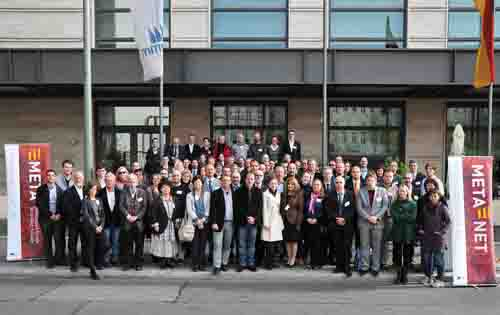
\includegraphics[width=\textwidth]{../_media/meta-net_team.jpg}
   %\fbox{Dummy -- we'll include the group photo of our META-NET meeting in Berlin here}
  \caption{Ligi 100 keeletehnoloogiaeksperti -- META-NETis osalevate maade ja keelte esindajad -- arutasid läbi ja viimistlesid selle valge raamatu sarja põhitulemused META-NETi koosolekul Berliinis 21. ja 22. oktoobril 2011.--- \textcolor{grey1}{About 100 language technology experts -- representatives of the countries and languages represented in META-NET -- discussed and finalised the key results and messages of the White Paper Series at a META-NET meeting in Berlin, Germany, on October 21/22, 2011.}}
\end{figure*}

\cleardoublepage

\bsection[META-NETi valge raamatu sari -- The META-NET White Paper Series]{META-NETi valge raamatu sari --- The META-NET\ \ \ \ \ \ White Paper Series}
\label{whitepaperseries}

\vspace*{-5mm}
\centering
  \setlength{\tabcolsep}{2em}
  \begin{tabularx}{\textwidth}{lllll} \toprule\addlinespace
  %\begin{tabulary}{170mm}{LLL} \toprule
  &baski & Basque & euskara& \\
  &bulgaaria & Bulgarian & български& \\
  &eesti & Estonian & eesti& \\ 
  &galiitsia & Galician & galego& \\
  &hispaania & Spanish & español& \\
  &hollandi & Dutch & Nederlands& \\  
  &horvaadi & Croatian & hrvatski& \\  
  &iiri & Irish & Gaeilge& \\
  &inglise & English & English& \\
  &islandi & Icelandic & íslenska& \\
  &itaalia & Italian & italiano& \\
  &katalaani & Catalan & català& \\ 
  &kreeka & Greek & ελληνικά& \\
  &leedu & Lithuanian & lietuvių kalba& \\
  &läti & Latvian & latviešu valoda& \\
  &malta & Maltese & Malti& \\
  &norra Bokmål & Norwegian Bokmål & bokmål& \\
  &norra Nynorsk & Norwegian Nynorsk & nynorsk& \\
  &poola & Polish & polski& \\
  &portugali & Portuguese & português& \\
  &prantsuse & French & français& \\  
  &rootsi & Swedish & svenska& \\  
  &rumeenia & Romanian & română& \\
  &saksa & German & Deutsch& \\ 
  &serbia & Serbian & српски& \\
  &slovaki & Slovak & slovenčina& \\
  &sloveeni & Slovene & slovenščina& \\
  &soome & Finnish & suomi& \\
  &taani & Danish & dansk& \\  
  &tšehhi & Czech & čeština& \\
  &ungari & Hungarian & magyar& \\ \addlinespace \bottomrule
\end{tabularx}
